%%%%%%%%%%%%%%%%%%%%%%%%%%%%%%%%%%%%%%%%%
% Masters/Doctoral Thesis 
% LaTeX Template
% Version 2.5 (27/8/17)
%
% This template was downloaded from:
% http://www.LaTeXTemplates.com
%
% Version 2.x major modifications by:
% Vel (vel@latextemplates.com)
%
% This template is based on a template by:
% Steve Gunn (http://users.ecs.soton.ac.uk/srg/softwaretools/document/templates/)
% Sunil Patel (http://www.sunilpatel.co.uk/thesis-template/)
%
% Template license:
% CC BY-NC-SA 3.0 (http://creativecommons.org/licenses/by-nc-sa/3.0/)
%
%%%%%%%%%%%%%%%%%%%%%%%%%%%%%%%%%%%%%%%%%

%----------------------------------------------------------------------------------------
%	PACKAGES AND OTHER DOCUMENT CONFIGURATIONS
%----------------------------------------------------------------------------------------

\documentclass[
11pt, % The default document font size, options: 10pt, 11pt, 12pt
%oneside, % Two side (alternating margins) for binding by default, uncomment to switch to one side
english, % ngerman for German
singlespacing, % Single line spacing, alternatives: onehalfspacing or doublespacing
%draft, % Uncomment to enable draft mode (no pictures, no links, overfull hboxes indicated)
%nolistspacing, % If the document is onehalfspacing or doublespacing, uncomment this to set spacing in lists to single
%liststotoc, % Uncomment to add the list of figures/tables/etc to the table of contents
%toctotoc, % Uncomment to add the main table of contents to the table of contents
%parskip, % Uncomment to add space between paragraphs
%nohyperref, % Uncomment to not load the hyperref package
headsepline, % Uncomment to get a line under the header
%chapterinoneline, % Uncomment to place the chapter title next to the number on one line
%consistentlayout, % Uncomment to change the layout of the declaration, abstract and acknowledgements pages to match the default layout
]{MastersDoctoralThesis} % The class file specifying the document structure
\usepackage[utf8]{inputenc} % Required for inputting international characters
\usepackage[T1]{fontenc} % Output font encoding for international characters
\usepackage{mathpazo} % Use the Palatino font by default
\usepackage{enumitem}
\usepackage{titlesec}
\usepackage{amsmath}
\usepackage[table,xcdraw]{xcolor}
\setcounter{secnumdepth}{4}
\titleformat{\paragraph}
{\normalfont\normalsize\bfseries}{\theparagraph}{1em}{}
\titlespacing*{\paragraph}
{0pt}{3.25ex plus 1ex minus .2ex}{1.5ex plus .2ex}
\usepackage{listings}
\usepackage{xcolor}
\lstset{
  basicstyle=\ttfamily,
  breaklines=true,
  backgroundcolor=\color{white},
  frame=single,
  columns=fullflexible
}
\usepackage{hyperref}
\hypersetup{
    colorlinks=true,
    linkcolor=blue,
    filecolor=magenta,      
    urlcolor=cyan,
    pdftitle={Overleaf Example},
    pdfpagemode=FullScreen,
    }

\usepackage[backend=bibtex,style=numeric,natbib=true]{biblatex} % Use the bibtex backend with the authoryear citation style (which resembles APA)
\addbibresource{references.bib} % The filename of the bibliography
\usepackage[autostyle=true]{csquotes} % Required to generate language-dependent quotes in the bibliography
\usepackage{booktabs,tabularx}
\renewcommand{\tabularxcolumn}{m}
\usepackage{multirow}
\usepackage{siunitx}

% Configure siunitx to round numbers to 4 significant figures
\sisetup{
  round-mode=figures,  % Round numbers to a certain number of significant figures
  round-precision=4    % Number of significant figures to retain
}
%\usepackage[section,strict]{placeins}
\usepackage{float}
%----------------------------------------------------------------------------------------
%	MARGIN SETTINGS
%----------------------------------------------------------------------------------------

\geometry{
	paper=a4paper, % Change to letterpaper for US letter
	inner=2.5cm, % Inner margin
	outer=3.8cm, % Outer margin
	bindingoffset=.5cm, % Binding offset
	top=1.5cm, % Top margin
	bottom=1.5cm, % Bottom margin
	%showframe, % Uncomment to show how the type block is set on the page
}

%----------------------------------------------------------------------------------------
%	THESIS INFORMATION
%----------------------------------------------------------------------------------------

\thesistitle{SPN: A novel neural network architecture to improve the performance of MLPs} % Your thesis title, this is used in the title and abstract, print it elsewhere with \ttitle
\supervisor{Dr. Phuong \textsc{T. Nguyen}} % Your supervisor's name, this is used in the title page, print it elsewhere with \supname
\examiner{} % Your examiner's name, this is not currently used anywhere in the template, print it elsewhere with \examname
\degree{Master of Science} % Your degree name, this is used in the title page and abstract, print it elsewhere with \degreename
\author{Sarosh \textsc{Krishan}} % Your name, this is used in the title page and abstract, print it elsewhere with \authorname
\addresses{} % Your address, this is not currently used anywhere in the template, print it elsewhere with \addressname

\subject{Computer Science} % Your subject area, this is not currently used anywhere in the template, print it elsewhere with \subjectname
\keywords{} % Keywords for your thesis, this is not currently used anywhere in the template, print it elsewhere with \keywordnames
\university{\href{https://www.univaq.it/en/}{University of L'Aquila}} % Your university's name and URL, this is used in the title page and abstract, print it elsewhere with \univname
\department{\href{http://www.disim.univaq.it/}{Department of Information Engineering, Information Sciences and Mathematics}} % Your department's name and URL, this is used in the title page and abstract, print it elsewhere with \deptname

\AtBeginDocument{
\hypersetup{pdftitle=\ttitle} % Set the PDF's title to your title
\hypersetup{pdfauthor=\authorname} % Set the PDF's author to your name
\hypersetup{pdfkeywords=\keywordnames} % Set the PDF's keywords to your keywords
}

\begin{document}

\frontmatter % Use roman page numbering style (i, ii, iii, iv...) for the pre-content pages

\pagestyle{plain} % Default to the plain heading style until the thesis style is called for the body content

%----------------------------------------------------------------------------------------
%	TITLE PAGE
%----------------------------------------------------------------------------------------

\begin{titlepage}
\begin{center}
\vspace*{.06\textheight}

\includegraphics[width=0.2\linewidth]{Figures/logos/univaq.pdf}

{\scshape\LARGE \univname\par}\vspace{1.5cm} % University name
\textsc{\Large Master Thesis}\\[0.5cm] % Thesis type
\HRule \\[0.4cm] % Horizontal line
{\huge \bfseries \ttitle\par}\vspace{0.4cm} % Thesis title
\HRule \\[1.5cm] % Horizontal line
\begin{minipage}[t]{0.4\textwidth}
\begin{flushleft} \large
\emph{Author:}\\
\href{https://github.com/lhamu}{\authorname} % Author name - remove the \href bracket to remove the link
\end{flushleft}
\end{minipage}
\begin{minipage}[t]{0.4\textwidth}
\begin{flushright} \large
\emph{Supervisor:} \\
\href{https://www.disim.univaq.it/ThanhPhuong}{\supname} % Supervisor name - remove the \href bracket to remove the link  
\end{flushright}
\end{minipage}\\[3cm]
\vfill
\large \textit{Corso di Laurea Magistrale in Informatica}\\[0.3cm] % 
%University 
%requirement text
\textit{}\\[0.4cm]
%\groupname\\
\deptname\\[0.5cm] % Research group name and department name
\vfill
{\large Academic Year 2024/2025}\\[2cm] % Date
%\includegraphics{Logo} % University/department logo - uncomment to place it
\vfill
\end{center}
\end{titlepage}

%----------------------------------------------------------------------------------------
%	DECLARATION PAGE
%----------------------------------------------------------------------------------------

\begin{center}
	% Erasmus Mundus Joint Master Degree Programme
	\vspace*{0.2\textheight}
	
	{\textbf{This thesis was conducted within the Erasmus Mundus Joint Master Degree Programme on the Engineering of Data-intensive Intelligent Software Systems (EDISS).}}

	% Add some vertical space before the image
	\vspace{2cm}

	% Include the larger logo image
	
\includegraphics[width=0.4\linewidth]{Figures/logos/EDISS_Transparent.png}

	% Add some vertical space after the image
	\vspace{2cm}
\end{center}


%----------------------------------------------------------------------------------------
%	ACKNOWLEDGEMENTS
%----------------------------------------------------------------------------------------

\begin{acknowledgements}
\addchaptertocentry{\acknowledgementname} % Add the acknowledgements to the table of contents
I would like to express my deep gratitude to my supervisor, Professor Phuong T. Nguyen, for his thoughtful advice, and support. His guidance has been indispensable throughout this process.

I would like to extend my thanks to EDISS programme coordinator Professor Sebastien Lafond and Professor Henry Muccini for providing me with this opportunity. Special thanks to Letizia Giorgetta for helping me navigate the intricacies of the administrative processes and always being ready to help.

I am incredibly blessed to have a wonderful support system of family and friends. I am extremely grateful to my parents Usha Bai and Krishan Lal, and my sisters Neev Kiran and Kiranti Krishan, for their love, unwavering support, and encouragement. 

\end{acknowledgements}

%----------------------------------------------------------------------------------------
%	LIST OF CONTENTS/FIGURES/TABLES PAGES
%----------------------------------------------------------------------------------------

\tableofcontents % Prints the main table of contents

\listoffigures % Prints the list of figures

\listoftables % Prints the list of tables

%----------------------------------------------------------------------------------------
%	ABBREVIATIONS
%----------------------------------------------------------------------------------------

\begin{abbreviations}{ll} % Include a list of abbreviations (a table of two columns)

\textbf{LAH} & \textbf{L}ist \textbf{A}bbreviations \textbf{H}ere\\
\textbf{WSF} & \textbf{W}hat (it) \textbf{S}tands \textbf{F}or\\

\end{abbreviations}

%----------------------------------------------------------------------------------------
%	THESIS CONTENT - CHAPTERS
%----------------------------------------------------------------------------------------

\mainmatter % Begin numeric (1,2,3...) page numbering

\pagestyle{thesis} % Return the page headers back to the "thesis" style

% Include the chapters of the thesis as separate files from the Chapters folder
% Uncomment the lines as you write the chapters

% Chapter 1

\chapter{Introduction} % Main chapter title

\label{Introduction} % For referencing the chapter elsewhere, use \ref{Chapter1} 

%----------------------------------------------------------------------------------------

% Define some commands to keep the formatting separated from the content 
\newcommand{\keyword}[1]{\textbf{#1}}
\newcommand{\tabhead}[1]{\textbf{#1}}
\newcommand{\code}[1]{\texttt{#1}}
\newcommand{\file}[1]{\texttt{\bfseries#1}}
\newcommand{\option}[1]{\texttt{\itshape#1}}

%----------------------------------------------------------------------------------------

The Perceptron, introduced by Frank Rosenblatt in 1958, is one of the earliest and most influential models in machine learning (ML). Designed to solve binary classification problems, the perceptron is a simple linear classifier inspired by the biological neurons in the human brain. It works by assigning weights to a set of input features and calculating a weighted sum of these features, which is passed through an activation function to determine the classification. The model iteratively adjusts these weights based on prediction errors, learning from the data until it reaches an optimal configuration.

However, while the perceptron performs well for linearly separable data, it struggles with more complex, non-linear problems. This limitation prompted the development of the Multi-Layer Perceptron (MLP) in the 1980s. MLPs extend the perceptron by adding multiple layers of perceptrons, enabling the model to learn non-linear relationships within the data. The breakthrough of backpropagation, introduced by Paul Werbos in the 1970s and popularized by Geoffrey Hinton and others in the 1980s, made it possible to train MLPs by calculating gradients and adjusting the weights across multiple layers.

The evolution of neural networks has given rise to specialized architectures such as Convolutional Neural Networks (CNNs) for image tasks and Transformer-based Large Language Models (LLMs) for natural language processing. Despite this, the MLP remains a foundational architecture that laid the groundwork for more advanced models. MLPs consist of multiple layers where each neuron in one layer is fully connected to every neuron in the subsequent layer, enabling the model to learn complex patterns in data, such as those found in image and speech recognition.

Recent research in neural network architecture design has evolved into a field known as Neural Architecture Search (NAS), which aims to find optimal architectures for a specific task by exploring various combinations of hyperparameters, layers, and connections. NAS employs search strategies, such as reinforcement learning, evolutionary algorithms, and gradient-based methods, to efficiently navigate the vast space of possible architectures. Despite the progress made, traditional MLPs are constrained by hierarchical connections between layers, which limit their ability to explore more flexible connectivity patterns, such as those involving skip connections within or between layers. While advancements like Residual Networks (ResNet) have introduced skip connections to alleviate this issue, the full potential of neuron connectivity remains untapped.

This thesis proposes a novel approach, Sarosh's Perceptron Networks (SPNs), to address these limitations by enabling unrestricted connectivity between neurons. Unlike traditional MLPs, SPNs eliminate the constraints on layer-to-layer connections, allowing neurons to interact more freely across the network. By fostering greater flexibility in connectivity, SPNs are hypothesized to enhance model performance without introducing the computational overhead typically associated with large, fully connected networks. This work aims to improve the expressiveness and efficiency of neural network architectures, offering new avenues for both theoretical exploration and practical applications in machine learning.


\section{Background and Motivation}
The Perceptron marked the first significant step in the evolution of artificial neural networks (ANNs). Rosenblatt’s model was inspired by the brain's structure, where neurons are connected by synapses and can adjust their strengths (synaptic weights) based on learning experiences. The Perceptron algorithm iterates over a set of input data, adjusts weights, and improves its ability to classify data. However, the perceptron could only solve problems that were linearly separable, leading to the need for more sophisticated architectures.

In the early 1980s, the Multi-Layer Perceptron (MLP) emerged, and the backpropagation algorithm was introduced to train these networks. Backpropagation allowed the MLPs to learn complex, non-linear functions by adjusting the weights across multiple layers using gradient descent. This innovation enabled the training of deep networks and formed the basis for modern deep learning techniques.

While MLPs were revolutionary, challenges remained regarding the optimal configuration of these networks. The number of layers and neurons in each layer, as well as how to connect these neurons, remained an open question. While the basic idea was that deeper networks (with more layers) could learn more complex patterns, no clear guidelines existed for how deep or wide the networks should be. Researchers began exploring empirical approaches to determine the ideal architecture.

One of the key insights came from "Efficient Backprop" (1998) by Yann LeCun, Léon Bottou, Geneviève Orr, and Klaus-Robert Müller, which highlighted methods for optimizing backpropagation. They proposed better weight initialization, momentum, and adaptive learning rates to accelerate convergence and prevent models from getting stuck in local minima. These methods made it possible to train deeper networks more effectively.

Further breakthroughs in architecture design came with Deep Residual Networks (ResNets), introduced in 2015 by Kaiming He and colleagues. ResNets utilized skip connections (residual blocks) that allowed information to bypass intermediate layers. This innovation solved the vanishing gradient problem, enabling the training of networks with hundreds or thousands of layers.

However, despite these advancements, the architectural design of neural networks remains an empirical challenge. Neural Architecture Search (NAS) emerged as an automated way to discover optimal architectures, but it is still computationally expensive and often depends on pre-existing knowledge.
%----------------------------------------------------------------------------------------

\section{Problem Statement}

Although MLPs and other deep learning models have made significant strides in various tasks, the design of their architecture remains a critical issue. Traditional MLPs suffer from a limited connectivity between neurons. Neurons within a single layer do not interact with one another, and neurons in different layers are connected only via intermediate neurons. This design limits the network's ability to learn complex, interdependent features in the data.

Despite advancements such as skip connections and residual networks, these solutions do not fully address the limitations of traditional MLP architectures. There is still a gap in the literature regarding the optimal arrangement of weights and neuron connectivity, which could potentially improve model performance, reduce training time, and allow for smaller, more efficient networks.
%----------------------------------------------------------------------------------------

\section{Research Gap and Contributions}

There is a significant gap in the literature concerning the optimization of neural network architectures, particularly in terms of neuron connectivity. Traditional MLPs rely on fixed architectural structures that restrict how neurons in different layers interact. Although skip connections have improved deep networks by mitigating the vanishing gradient problem, they still impose certain constraints, such as requiring neurons to have the same dimensionality or limiting connections to adjacent layers.

This thesis introduces Denser Perceptron Networks (DPNs), a new framework that eliminates the restriction of fixed connectivity patterns between neurons. DPNs allow for fully connected networks, where any two neurons can be linked. This increased connectivity has the potential to improve the model’s ability to learn complex, interdependent features, potentially leading to improved generalization and performance.

The main contributions of this thesis are:

The introduction of DPNs: A new neural network architecture that eliminates the restrictions of traditional MLP designs.

Empirical evaluation: A comparison of DPNs with traditional MLPs to determine whether the increased connectivity results in better performance, faster training, and more efficient models.

Improved training efficiency: Investigation into whether DPNs can achieve high performance while reducing the time and memory costs typically associated with larger, deeper networks.

%----------------------------------------------------------------------------------------

\section{Research Questions}

\begin{enumerate}[label={RQ\arabic*.}, leftmargin=*]
    \item Do Sarosh's Perceptron Networks (SPNs) achieve better model performance than traditional Multi-Layer Perceptrons (MLPs)? \label{RQ1}
    \item Does removing connectivity restrictions in neural networks enhance the learning capability of MLPs? \label{RQ2}
    \item Can SPNs maintain strong performance with smaller network sizes, thus improving computational efficiency? \label{RQ3}
    \item How do SPNs compare to traditional MLPs in terms of training time, memory usage, and model accuracy? \label{RQ4}
    \item How does the increased flexibility of SPNs influence their ability to generalize across various datasets and tasks? \label{RQ5}
    \item Can the high performance of fully connected SPNs be retained after optimization and reduction of connectivity, thereby achieving better computational efficiency and faster training times? \label{RQ6}
\end{enumerate}

%----------------------------------------------------------------------------------------

\section{Scope and Limitations}

This research focuses on Denser Perceptron Networks (DPNs) and evaluates their potential to enhance neural network performance through improved connectivity. The scope of the thesis is limited to the empirical comparison of DPNs with traditional MLPs on classification tasks.

Key limitations include:

Computational Constraints: DPNs, by design, involve a large number of connections, which may result in higher computational demands for training and inference. This research will focus on evaluating whether the performance gains from DPNs justify the computational cost.

Task-specific Design: The results of this study may vary depending on the dataset and task. While the thesis focuses on classification tasks, the generalizability of DPNs to other types of tasks may require further investigation.

Data Constraints: The experiments will be conducted using a set of standard datasets, and the findings may not fully apply to more complex or diverse real-world data.

%----------------------------------------------------------------------------------------


\section{Thesis Structure and Overview}

The remainder of this thesis is organized as follows:
\begin{enumerate}
    \item Chapter \ref{LiteratureReview} presents a literature review on the existing research on continual learning and the different methods proposed for the mitigation of catastrophic forgetting.
    \item Chapter \ref{Methodology} describes the methodology used in the research, including the method for data preparation, preprocessing, fine-tuning, implementation of the mitigation approach, and the evaluation with different benchmarks.
    \item Chapter \ref{Experiments} describes the different experiments carried out as part of this study, along with the different ablations performed.
    \item Chapter \ref{Results} involves the analysis of the results obtained from the experiments.
    \item Chapter \ref{Conclusion} summarizes the findings of the thesis work and suggests directions for future work.

\end{enumerate}
% Chapter Template

\chapter{Literature Review} % Main chapter title

\label{LiteratureReview} % Change X to a consecutive number; for referencing this chapter elsewhere, use \ref{ChapterX}

%----------------------------------------------------------------------------------------
%	SECTION 1
%----------------------------------------------------------------------------------------

\section{Neural Architecture Search (NAS)}

Neural Architecture Search (NAS) is an automated method for optimizing neural network architectures. The primary objective of NAS is to find an optimal architecture that provides the best trade-off between model performance (accuracy) and resource usage (computational efficiency, parameter count, and memory usage) \cite{elsken2019neural}. NAS has significantly contributed to the advancement of deep learning by automating architecture design, traditionally a manually intensive process.
%-----------------------------------
%	SUBSECTION 1
%-----------------------------------
\subsection{Current Techniques in NAS}

NAS techniques are broadly categorized into reinforcement learning (RL)-based methods, evolutionary algorithms (EA), and gradient-based optimization methods.

\textbf{Reinforcement Learning-based NAS} techniques use an RL agent that generates neural architectures and updates its strategy based on rewards from evaluating the architectures \cite{zoph2016neural}. Notable examples include the work by Zoph and Le, where an RNN controller designs neural architectures \cite{zoph2016neural}.

\textbf{Evolutionary Algorithm-based NAS} methods use population-based optimization inspired by biological evolution, including mutation, crossover, and selection to evolve architectures \cite{real2019regularized}. Real et al. demonstrated that evolutionary methods could effectively evolve architectures that outperform manually designed ones \cite{real2019regularized}.

\textbf{Gradient-based NAS} methods, such as Differentiable Architecture Search (DARTS), formulate NAS as a continuous optimization problem, allowing for efficient gradient-based optimization \cite{liu2018darts}. DARTS has become popular due to its efficiency in discovering competitive architectures with lower computational cost.

\begin{table}[ht]
\centering
\caption{Comparison of NAS Techniques}
\begin{tabular}{|c|c|c|}
\hline
\textbf{Technique} & \textbf{Advantages} & \textbf{Disadvantages} \\
\hline
RL-based & High flexibility & Computationally expensive \\
\hline
EA-based & Effective global search & Requires extensive evaluations \\
\hline
Gradient-based & Efficient and scalable & Sensitive to initialization \\
\hline
\end{tabular}
\label{tab:nas_techniques}
\end{table}

%----------------------------------------------------------------------------------------
%	SECTION 2
%----------------------------------------------------------------------------------------

\section{Multi-Layer Perceptrons (MLPs)}
Multi-Layer Perceptrons (MLPs) are classical feedforward artificial neural networks composed of multiple layers of nodes (neurons). Each node employs a non-linear activation function enabling the network to learn complex patterns through supervised learning techniques, such as backpropagation \cite{rumelhart1986learning}. MLPs have traditionally served as baseline models due to their simplicity and general applicability across diverse tasks, including classification and regression problems.

However, MLPs typically suffer from issues such as overfitting and computational inefficiency when scaling to deeper and wider networks. This motivates research into improving the architectural efficiency and effectiveness of MLPs through enhanced connectivity, optimized neuron allocation, and specialized training procedures.

\section{Pruning in Neural Networks}
Pruning is a method to reduce network complexity by eliminating redundant connections or neurons, effectively improving computational efficiency without significantly compromising performance \cite{han2015learning}. It seeks to achieve sparsity within the network, reducing the model size, memory footprint, and inference latency, thus facilitating deployment in resource-constrained environments.

Pruning methods can be classified into magnitude-based, structure-based, and learning-based pruning:

\textbf{Magnitude-based pruning} involves removing weights based on their absolute magnitude, assuming low-magnitude weights contribute less to the network's predictive capability \cite{han2015learning}.

\textbf{Structured pruning} removes entire channels or layers, maintaining regular structure beneficial for hardware acceleration \cite{he2017channel}.

\textbf{Learning-based pruning}, such as iterative magnitude pruning, incrementally prunes the network while retraining it to recover accuracy \cite{han2015learning}.

\section{Lottery Ticket Hypothesis}
The Lottery Ticket Hypothesis, proposed by Frankle and Carbin, posits that dense, randomly-initialized neural networks contain smaller subnetworks (winning tickets) which, when trained in isolation, can match or exceed the test accuracy of the original network \cite{frankle2018lottery}.

This hypothesis suggests that initialization plays a crucial role in neural network training. Frankle and Carbin’s pruning approach involves:
\begin{enumerate}
\item Training the original network fully.
\item Pruning a fraction of the lowest magnitude weights.
\item Resetting the remaining weights to their initial values.
\item Repeating this iterative process multiple times.
\end{enumerate}

The Lottery Ticket Hypothesis has provided a theoretical and empirical foundation for understanding network pruning and initialization strategies. It emphasizes the importance of structured pruning approaches, challenging the traditional random pruning practices.

\section{Summary}
This literature review highlights the advancements in neural architecture optimization through NAS, the foundational structure and limitations of MLPs, and the efficacy of pruning methods, particularly through the lens of the Lottery Ticket Hypothesis. These areas collectively inform strategies for improving neural network performance and efficiency, forming the theoretical underpinning of the current research. 
% Chapter Template

\chapter{Methodology} % Main chapter title

\label{Methodology} % Change X to a consecutive number; for referencing this chapter elsewhere, use \ref{ChapterX}

%----------------------------------------------------------------------------------------
%	SECTION 1
%----------------------------------------------------------------------------------------

\section{Sarosh's Perceptron Networks (SPNs)}

This chapter introduces the theoretical framework for Sarosh's Perceptron Networks (SPNs), designed to eliminate restrictions on neuron connectivity. The goal is to allow any two neurons to connect, forming a directed acyclic graph (DAG) like network (since cycles would cause deadlocks). This framework seeks to enhance neural networks by improving their connectivity while minimizing the associated increases in time and space complexities.
 
In theory, SPNs treat neurons as individual objects that can process inputs independently. These neurons may still depend on either the input data or other neurons for input, but the framework enables greater flexibility in forming connections across the network. Figure \ref{fig:exampleSPN} illustrates an arbitrary eample of such a network.

\begin{figure}[h!]
\centering
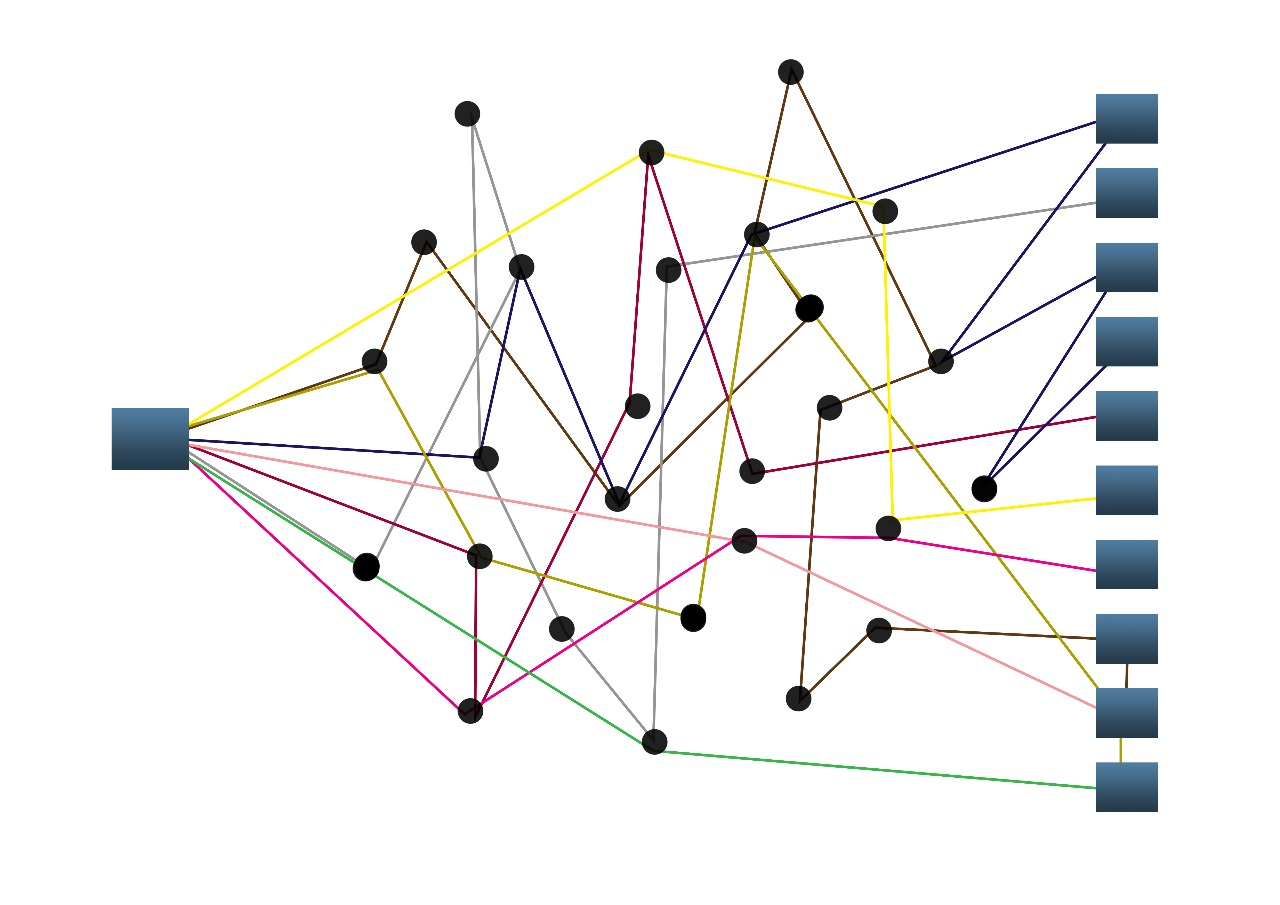
\includegraphics[width=0.7\textwidth]{Figures/Methodology/example_spn.jpg}
\caption{An Example SPN Network.}
\label{fig:exampleSPN}
\end{figure}

%-----------------------------------
%	SUBSECTION 1
%-----------------------------------
\subsection{Connection vs Neuron}

Before defining connectivity, it is important to clarify what is meant by a \emph{connection}. As illustrated in Figure \ref{fig:perceptronArch}, a perceptron (used interchangeably with "neuron" throughout this thesis) receives multiple inputs, each of which is assigned a learnable weight. The perceptron computes a weighted sum of its inputs, adds a learnable bias term, and passes the result through an activation function. In this thesis, a \textbf{connection} is defined as any instance where an input transmits its value to a given perceptron. Each connection introduces a new learnable weight parameter for that perceptron, thereby increasing the overall parameter count of the network by one per connection.

\begin{figure}[h!]
\centering
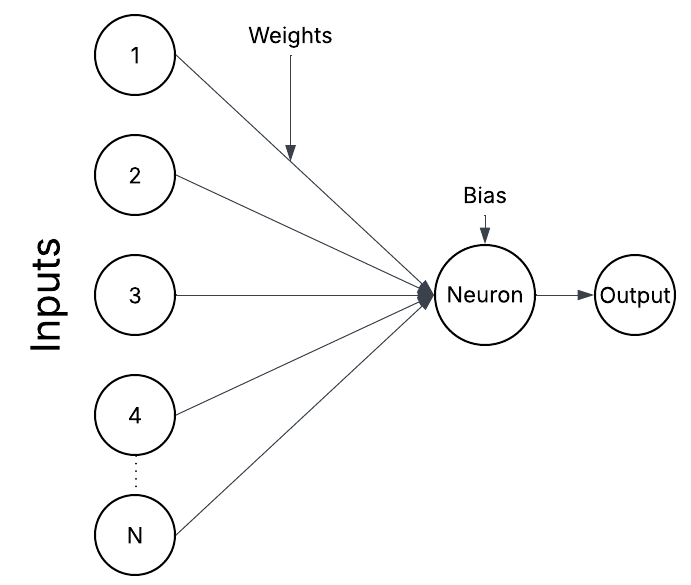
\includegraphics[width=0.4\textwidth, height=0.2\textheight]{Figures/Methodology/perceptron_architecture.png}
\caption{Architecture of a single Perceptron.}
\label{fig:perceptronArch}
\end{figure}

Accordingly, a Multi-Layer Perceptron is defined as a network composed of multiple layers of perceptrons. Thus, SPNs focuses on increasing the connection density of MLP models, while retaining the original number of neurons.

\subsection{Motivation for SPNs}

As illustrated in Figure \ref{fig:mlpStructure}, a typical MLP architecture features sequential connectivity: every neuron in a given layer is fully connected to all neurons in the subsequent layer. However, this conventional design omits two important types of connections.

\begin{figure}[h!]
\centering
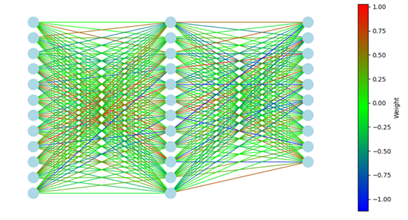
\includegraphics[width=0.7\textwidth]{Figures/Methodology/mlp_structural_diagram.png}
\caption{Low level illustration of an MLP.}
\label{fig:mlpStructure}
\end{figure}


\begin{enumerate}
    \item \textbf{Cross-layer connections} (shown in Figure \ref{fig:crossLayerConnection}): These connections would allow a layer to link to any preceding layer, not just the one immediately behind it.
    \begin{figure}[h!]
    \centering
    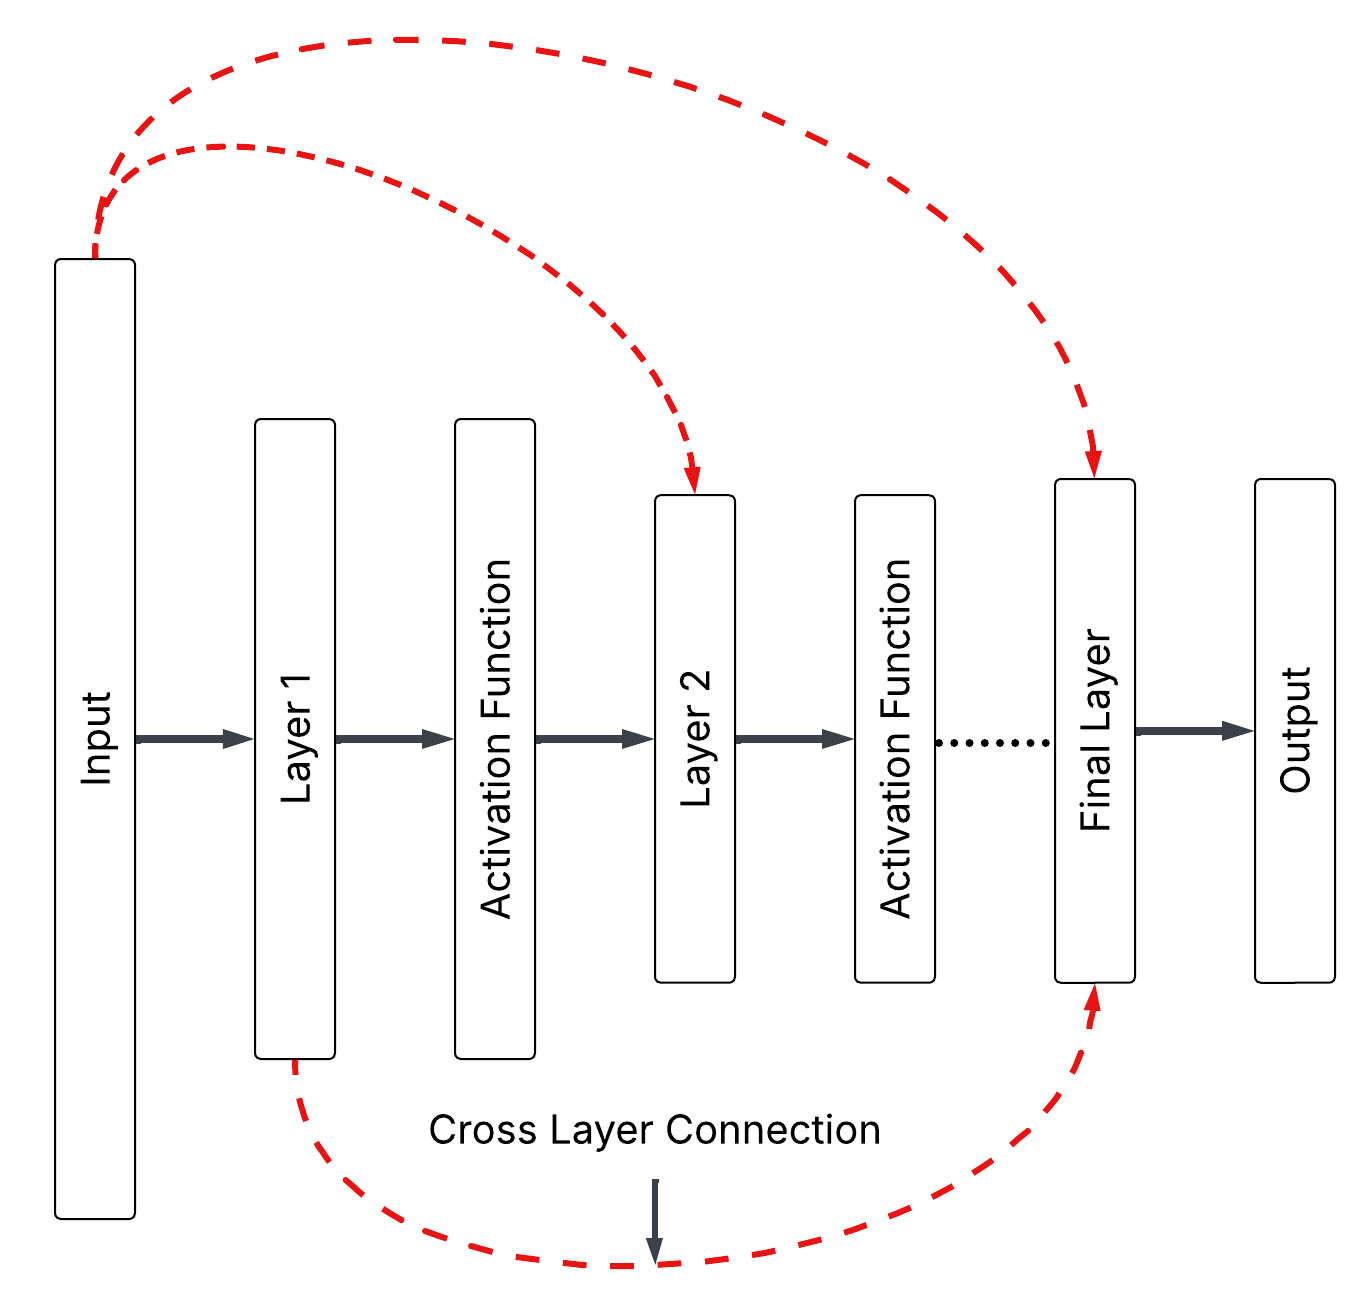
\includegraphics[width=0.7\textwidth]{Figures/Methodology/cross_layer_connections.png}
    \caption{Missing cross layer connections in MLP.}
    \label{fig:crossLayerConnection}
    \end{figure}

    \item \textbf{Intra-layer connections} (depicted in Figure \ref{fig:intraLayerConnection}): These would enable neurons within the same layer to connect to each other, a feature absent in standard MLPs.
    
    \begin{figure}[h!]
    \centering
    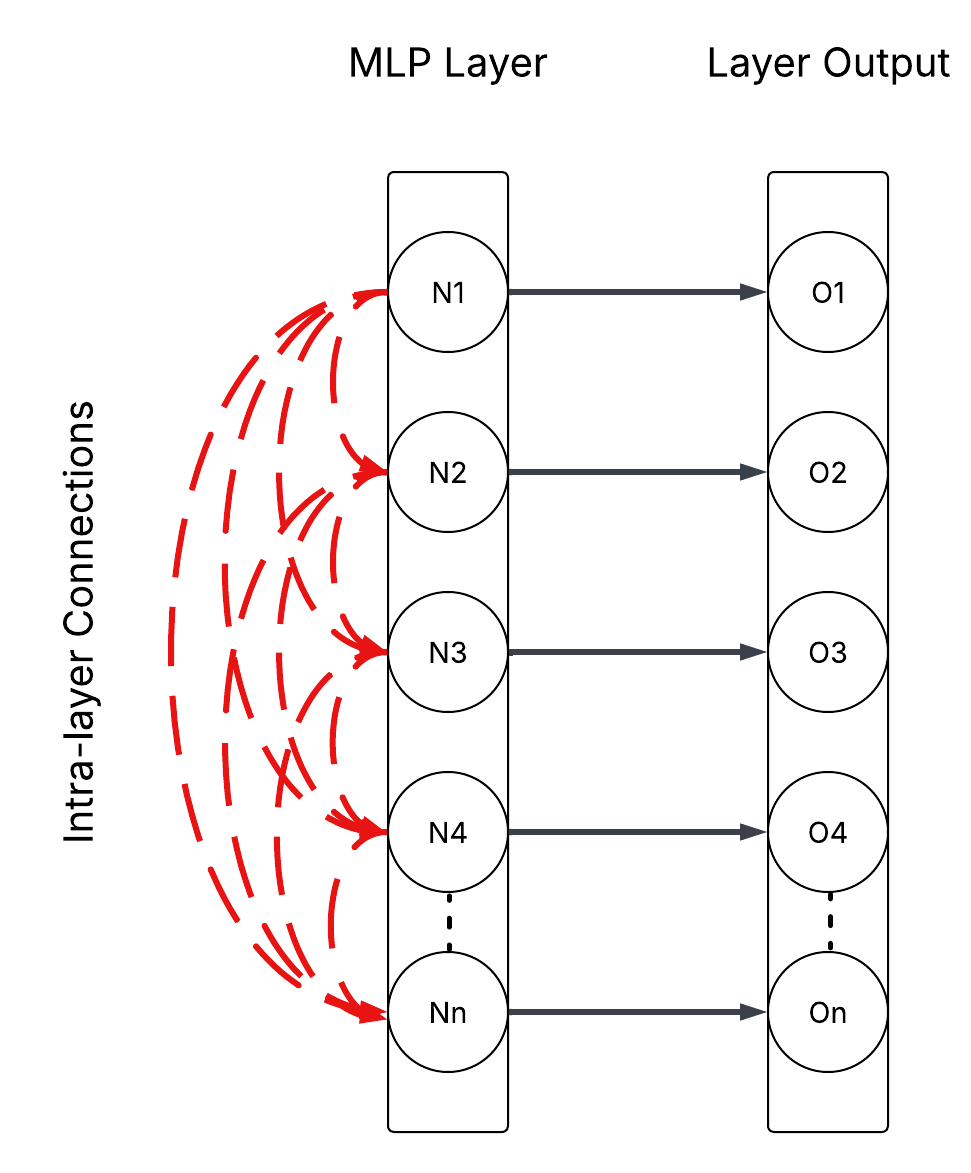
\includegraphics[width=0.5\textwidth, height=0.4\textheight]{Figures/Methodology/intra_layer_connections.png}
    \caption{Missing Intra-layer connections in a single MLP layer.}
    \label{fig:intraLayerConnection}
\end{figure}

\end{enumerate}

Alternatively, the weights of an MLP can be represented as a single, large weight matrix, where the x-axis corresponds to the input features and the y-axis to the neurons containing these weights, as illustrated in Figure \ref{fig:mlpWeights}. In the illustration, every layer is assumed to compose of only two neurons. 

\begin{figure}[h!]
\centering
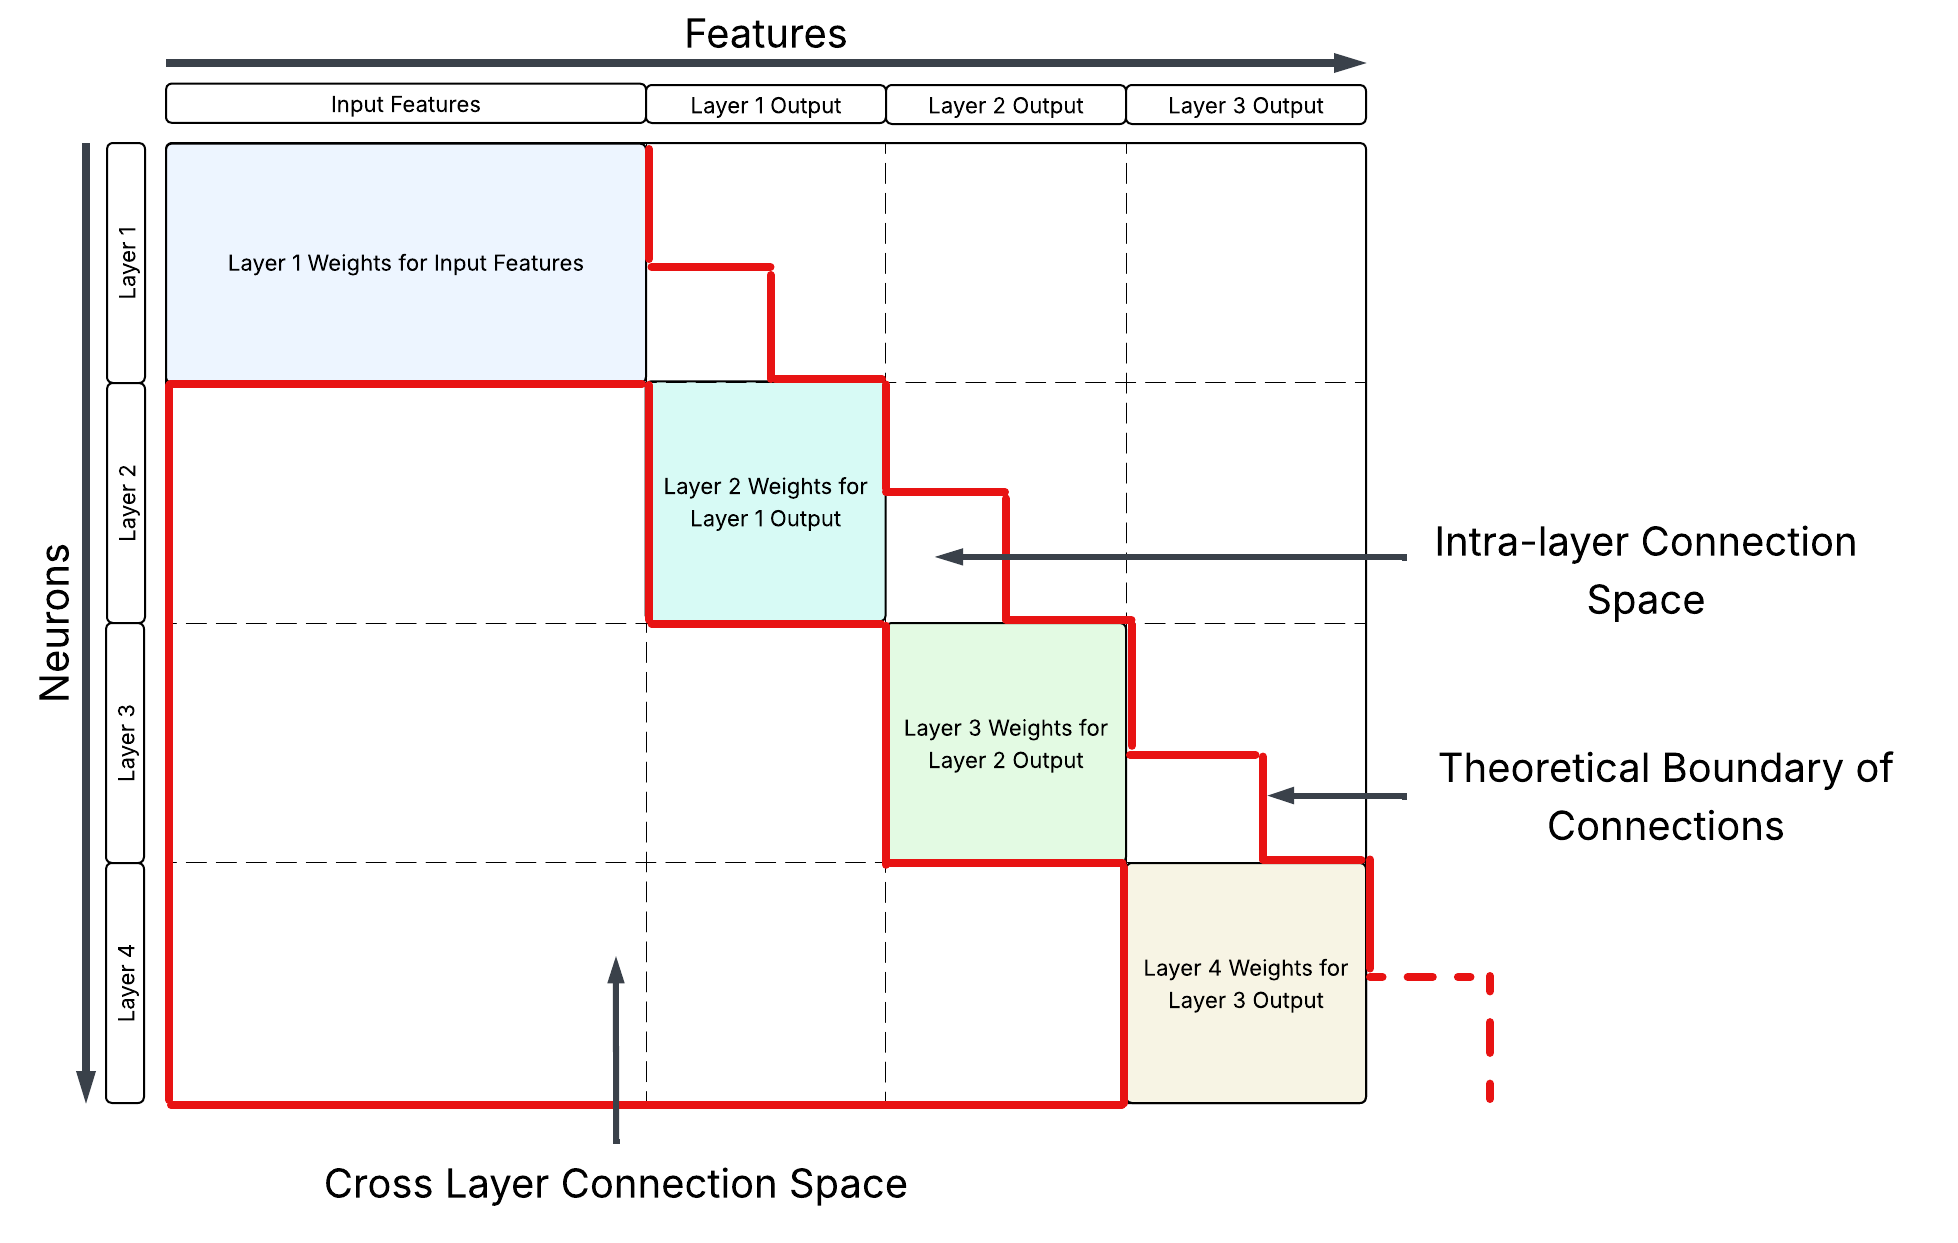
\includegraphics[width=1.0\textwidth]{Figures/Methodology/mlp_weight_matrix.png}
\caption{Cross Layer Connection Space and Intra-layer connection space with the theoretical connection boundary in the combined weight matrix of a traditiona MLP, assuming each layer has two neurons.}
\label{fig:mlpWeights}
\end{figure}

In the representation in Figure \ref{fig:mlpWeights}, the nonzero weights appear in diagonal arragned blocks, forming a staircase-like pattern that is separated along both axes. On the right side of the boxes, there is a theoretical boundary of connections. If any connections cross this boundary, it would form a cycle within the network where a neuron would be connected to itself (dependent on its own output). Thus, this boundary can never be crossed.

This visualization also makes it evident that both the left and right regions outside the blocks are completely empty. The empty region on the left corresponds to the absence of cross-layer connections, while the empty region on the right reflects the lack of intra-layer connections within the same layer.

Examining the weight matrix further, we notice that the right side of the matrix effectively determines the model’s number of layers. If we begin populating this region by introducing intra-layer connections, we break the independence that typically defines neurons within the same layer. Adding this dependency thus splits the original layer into multiple distinct layers. Intuitively, this aligns with the conventional understanding that neurons within a layer should not interact directly.

Adding weights to either the left or right of the existent MLP blocks transforms the classic MLP structure into a Sarosh’s Perceptron Network.

\subsection{Free Weight SPNs}

In the MLP weight matrix shown in Figure \ref{fig:mlpStructure}, adding connections to the left side of the matrix does not increase the model's layer count. This is crucial as the number of layers in a model determines how many times the input is processed before producing an output, and thus directly relates to the model’s throughput. Therefore, incorporating weights on the left side of the matrix maximizes the possible connections within the given layer structure without impacting throughput. Therefore, these additional connections are termed “Free Weights”, as they can be added without any cost to the model's throughput. 

Incorporating free weights into traditional MLPs is analogous to concatenating the output of a layer with its input before passing it to the next layer. This approach increases the space complexity of the MLP by $\mathcal{O}(l^2)$, while maintaining a time complexity of $\mathcal{O}(l)$, where $l$ is the number of layers. A key advantage of this method is that subsequent layers can learn from both the original input and features extracted by previous layers, allowing the network to capture more complex and nuanced patterns.

An MLP enhanced with Free Weights is then referred to as a Free Weights SPN.

\begin{figure}[h!]
\centering
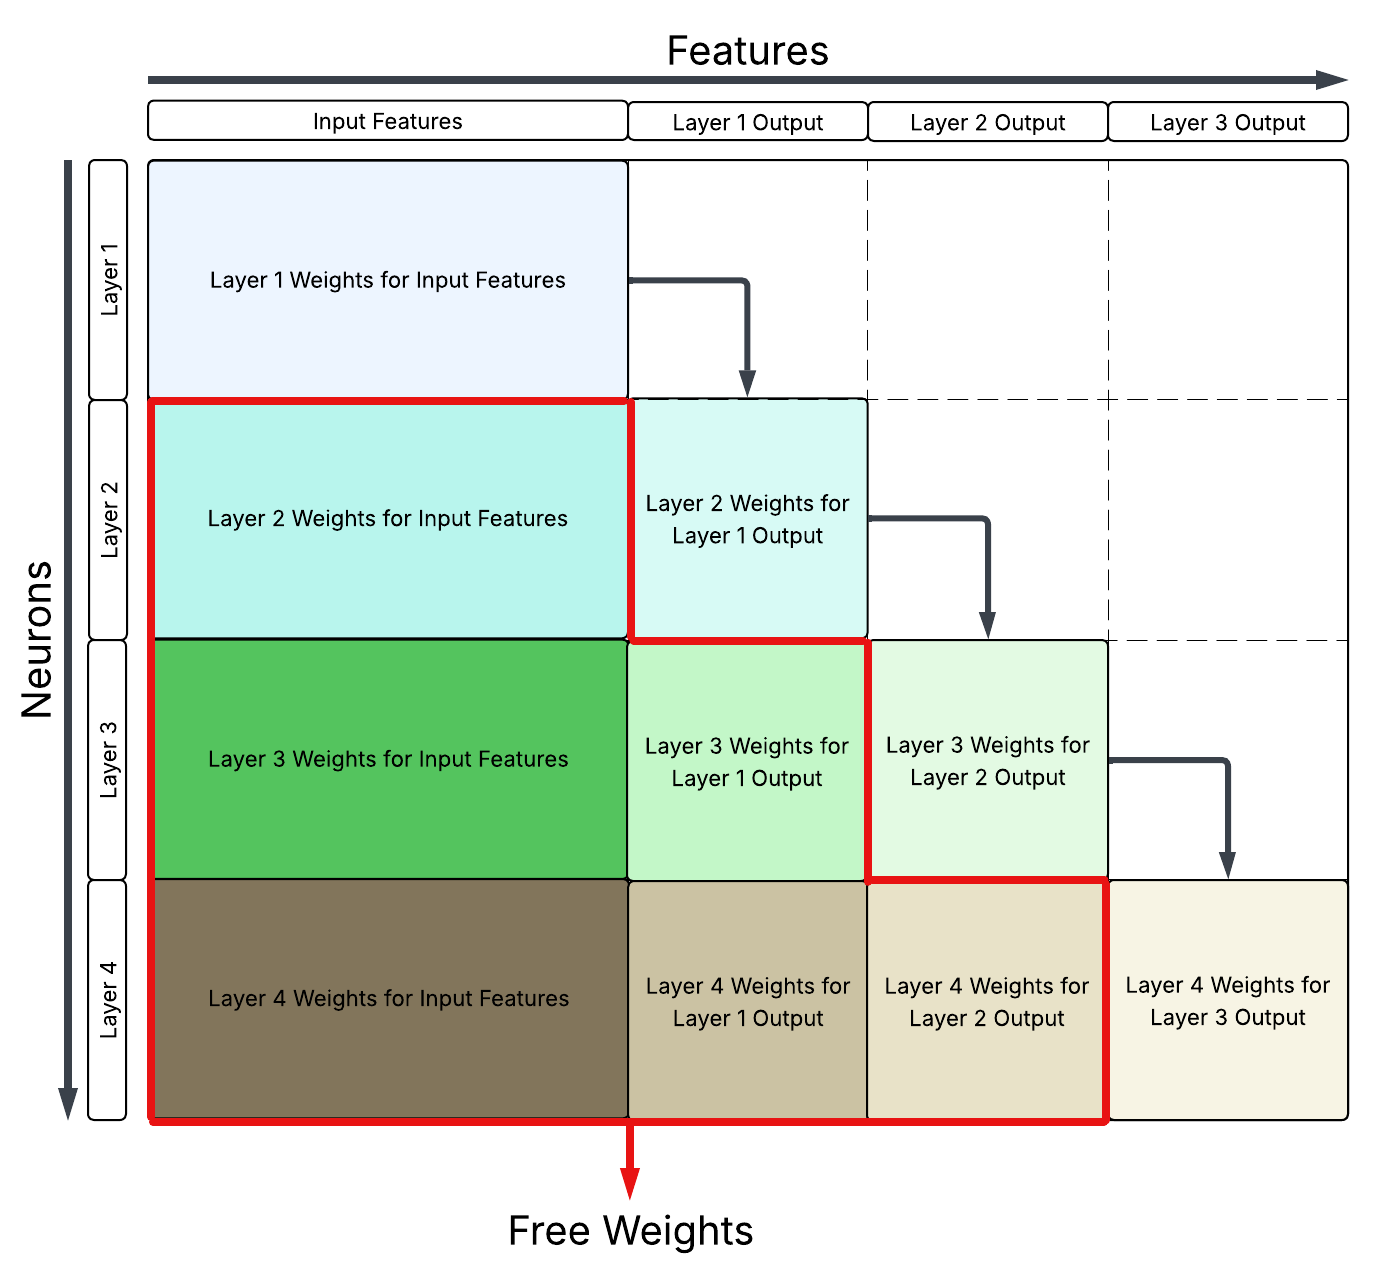
\includegraphics[width=0.7\textwidth]{Figures/Methodology/Free_Weights_SPN_Weights.png}
\caption{Illustration of a traditional MLP with Free Weights.}
\label{fig:fwSpn}
\end{figure}

\subsection{Maximal SPNs}

Additionally, by adding weights to the right side of the diagonal blocks, the weight matrix becomes a fully filled staircase pattern, with each "step" corresponding to a single neuron. This configuration not only maximizes the number of possible connections but also increases the layer count to match the total number of neurons, thereby minimizing the model’s throughput. Such a model, which achieves both maximal connectivity and maximal depth, is referred to as a Maximal SPN.

\begin{itemize}
    \item Time complexity of Maximal SPNs: $\mathcal{O}(n)$, since every neuron becomes its own layer
    \item Space complexity: Using $I$ as the number of features in the input data and $n$ as the number of neurons.
    \begin{align*}
    =\, & I + (I+1) + (I+2) + \dots + (I + n - 1) \\
    =\, & I \cdot (1 + 2 + \dots + (n-1)) \\
    =\, & I \cdot \frac{n(n-1)}{2} \\
    =\, & \mathcal{O}(I \cdot n^2)
    \end{align*}
\end{itemize}

\begin{figure}[h!]
\centering
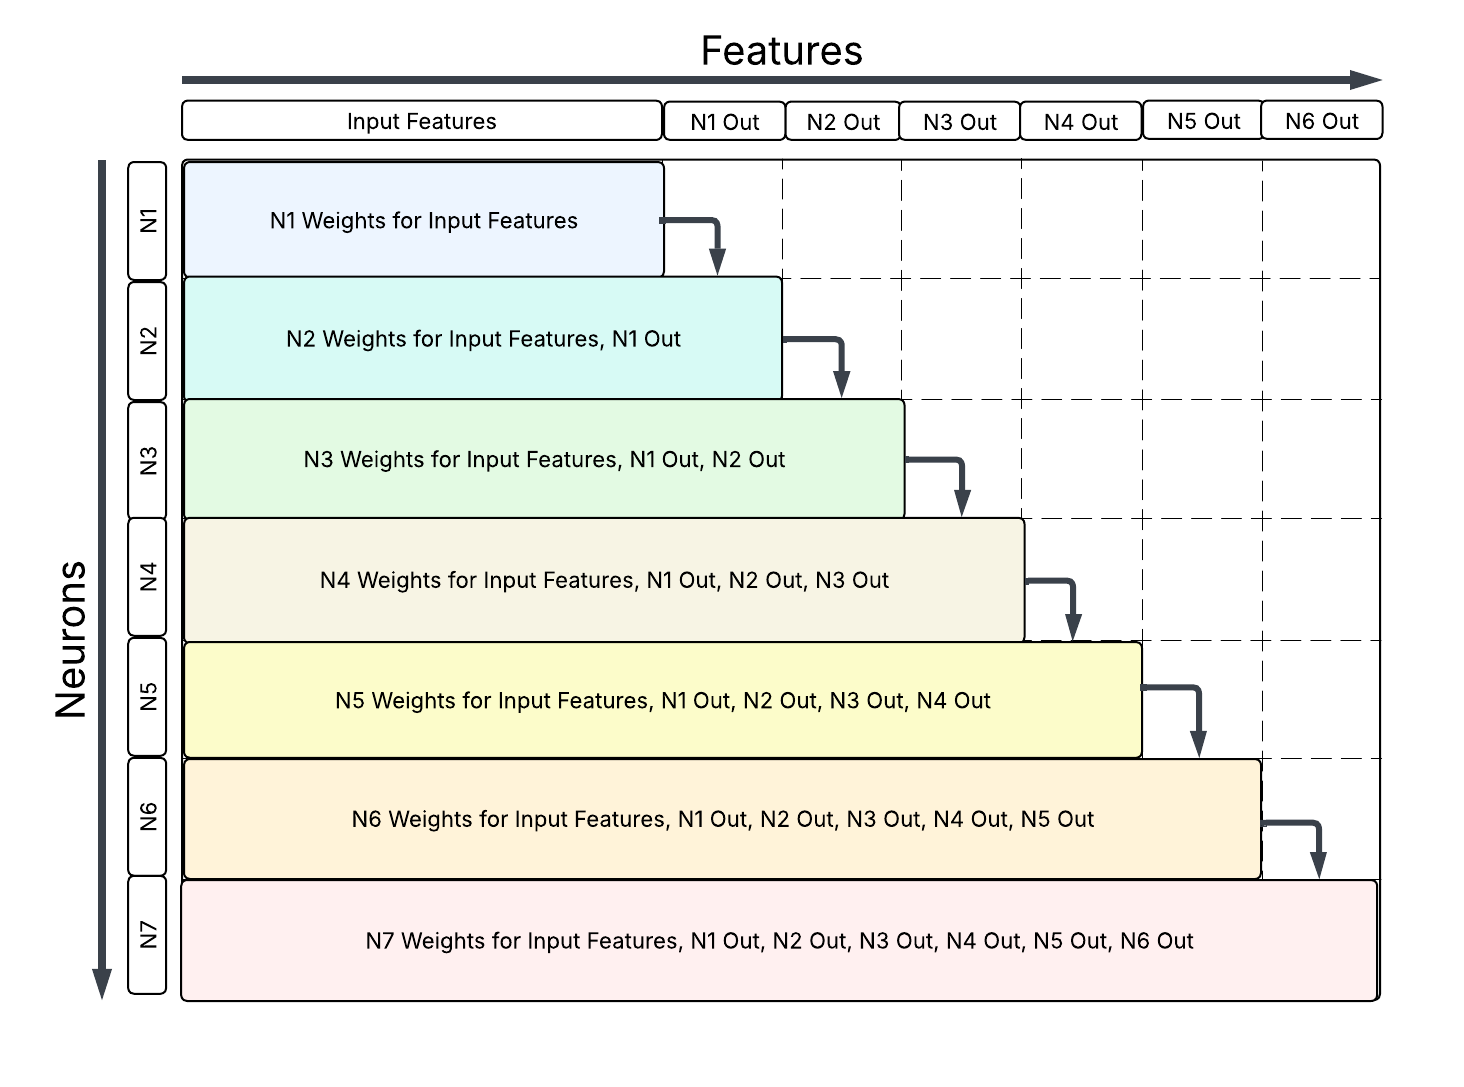
\includegraphics[width=0.7\textwidth]{Figures/Methodology/Neuron_Based_Maximal_SPN_Weights.png}
\caption{Illustration of a Maximal SPN.}
\label{fig:maxSpn}
\end{figure}

%-----------------------------------
%	SUBSECTION 2
%-----------------------------------

\subsection{Pruned Maximal SPNs}

Since maximal SPNs can have an excessive number of layers and consequently, poor throughput, one potential solution is \textbf{pruning}. The Lottery Ticket Hypothesis posits that over 90\% of weights in a network can be removed while still achieving performance comparable to the original network, suggesting the existence of a subnetwork within the initial network that is equally trainable~\cite{frankle2018lottery}.

Applying this principle, if we prune a maximal SPN, zeroing out selected weights on the rightmost edges of the staircase weight matrix, we effectively reduce dependencies between certain neurons as illustrated in Figure \ref{fig:pruningMaxSPN}. This reduction allows for the merging of independent neurons into shared layers, thus reintroducing parallelism to the network while maintaining its high expressiveness and capacity for learning complex data patterns.

\begin{figure}[h!]
\centering
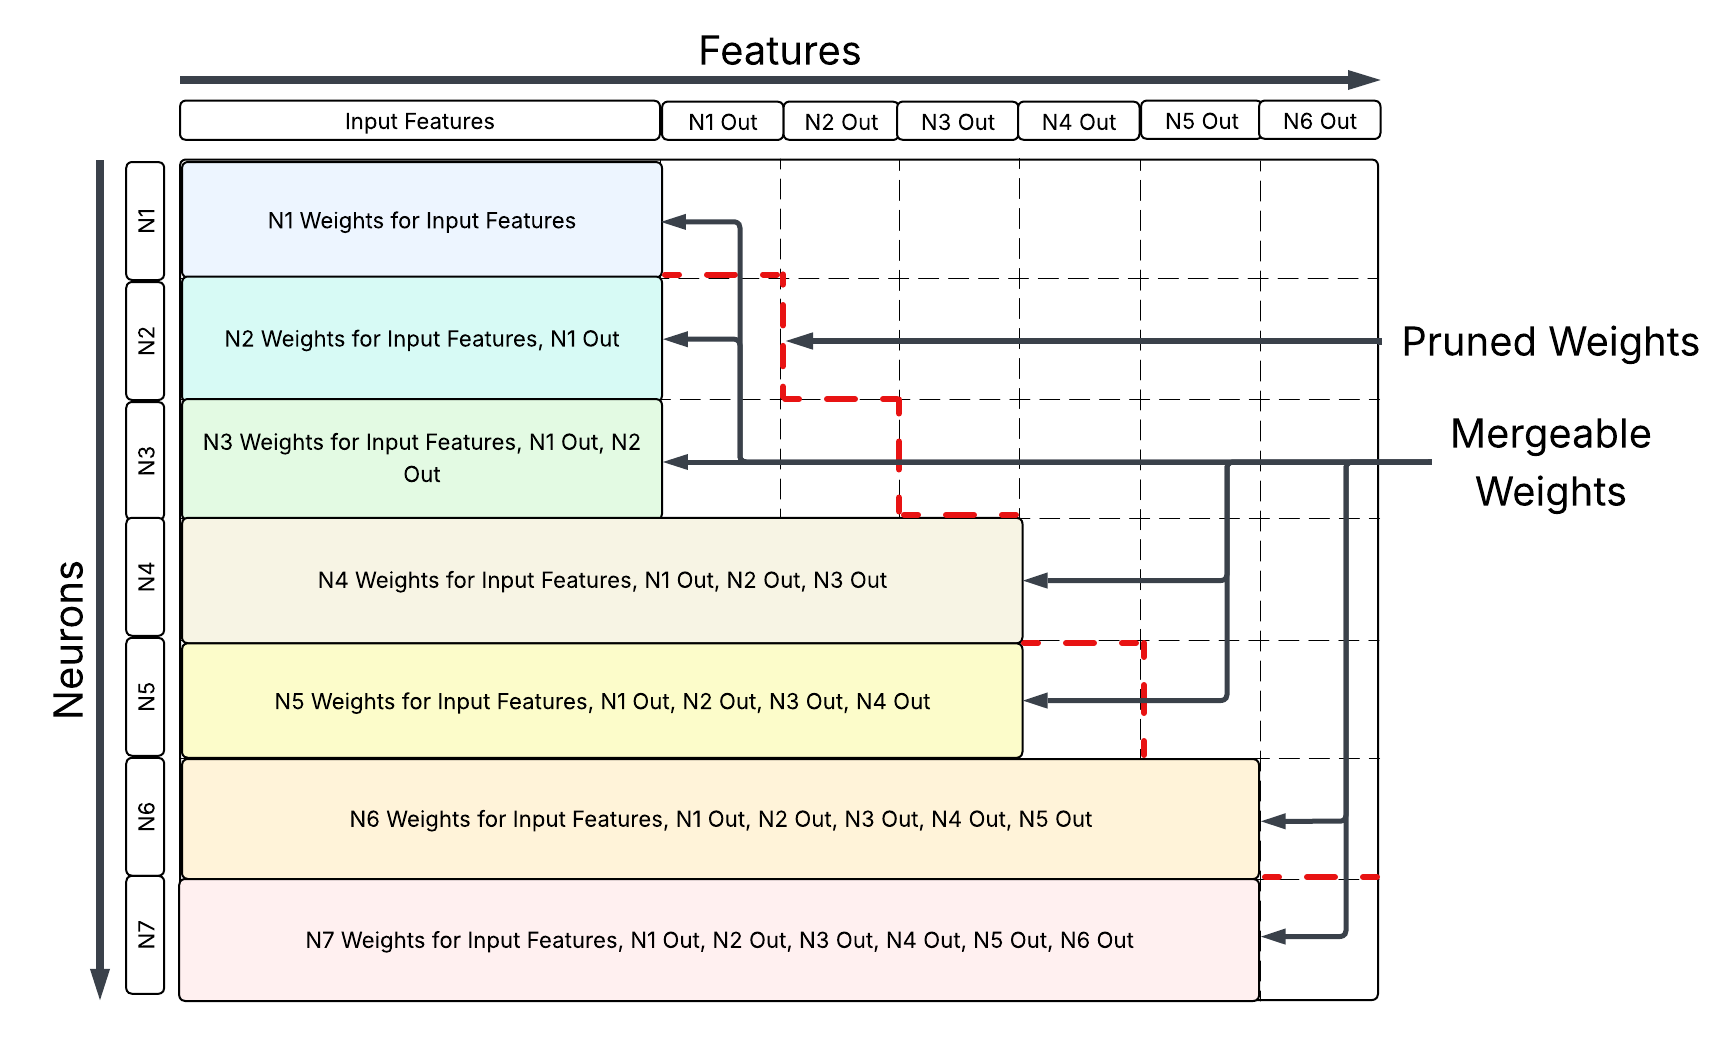
\includegraphics[width=0.7\textwidth]{Figures/Methodology/pruning_max_spn.png}
\caption{Pruning a Maximal SPN.}
\label{fig:pruningMaxSPN}
\end{figure}

The pruning strategy adopted in the current SPN framework is inspired by the Lottery Ticket Hypothesis and follows these steps:
\begin{enumerate}
    \item Train the original network to completion.
    \item Prune a fraction of the weights with the lowest magnitudes.
    \item Reset the remaining weights to their initial values.
    \item Repeat this process iteratively for several cycles.
\end{enumerate}

This iterative process is repeated for a user-defined number of rounds, with the optimal number typically determined through empirical testing or validation. In each round, a fraction of the model’s lowest-magnitude weights are pruned, and the initial weights yielding the best performance are retained. This continues until up to 99\% of the weights have been removed. At the end of the process, the best-performing set of initial weights is used to construct the final pruned model.

At the conclusion of this procedure, neurons that have become independent as a result of pruning are merged to reduce the overall layer count and improve throughput. It is important to note that merging is performed only after the entire pruning process has finished. Preliminary experiments revealed that merging neurons during pruning can alter the network's architecture in ways that negatively affect subsequent pruning steps, making the overall process less effective than waiting until pruning is complete.

\subsection{Minimal SPNs}

At the other end of the spectrum, if our goal is to minimize the number of layers while maximizing connectivity, we arrive at the concept of minimal SPNs. This involves organizing the network with as few layers as possible and enriching them with free weights.

Theoretically, the most minimal architecture would be a single perceptron, or for multiclass classification, a single layer with as many neurons as there are output classes ($o$). However, for this analysis, we assume a fixed total number of neurons ($n$) and seek to arrange them into layers to minimize throughput. This leads to two possible scenarios:

\begin{enumerate}
    \item When the total number of neurons equals the output size ($n = o$): Only a single output layer of size $o$ is possible, with no opportunity for cross-layer connections.
    \item When the total number of neurons exceeds the output size ($n > o$): The network can be organized into two layers: an output layer of size $o$ and a hidden layer with the remaining $n-o$ neurons. This configuration yields a minimal MLP, as illustrated in Figure \ref{fig:minMLP}. By introducing free weights, we transform it into a minimal SPN, depicted in Figure \ref{fig:minSpn}.
\end{enumerate}

\begin{itemize}
    \item Time complexity: $\mathcal{O}(1)$, since there can always be a maximum of two layers, the time complexity is constant.
    \item Space complexity: Using $I$ as the number of features in the input data and $n$ as the number of neurons.
    \begin{align*}
    =\, & I \cdot (n) + n \cdot o \\
    =\, & \mathcal{O}(I \cdot n)
    \end{align*}
\end{itemize}

\begin{figure}[h!]
    \centering
    \begin{minipage}[t]{0.48\textwidth}
        \centering
        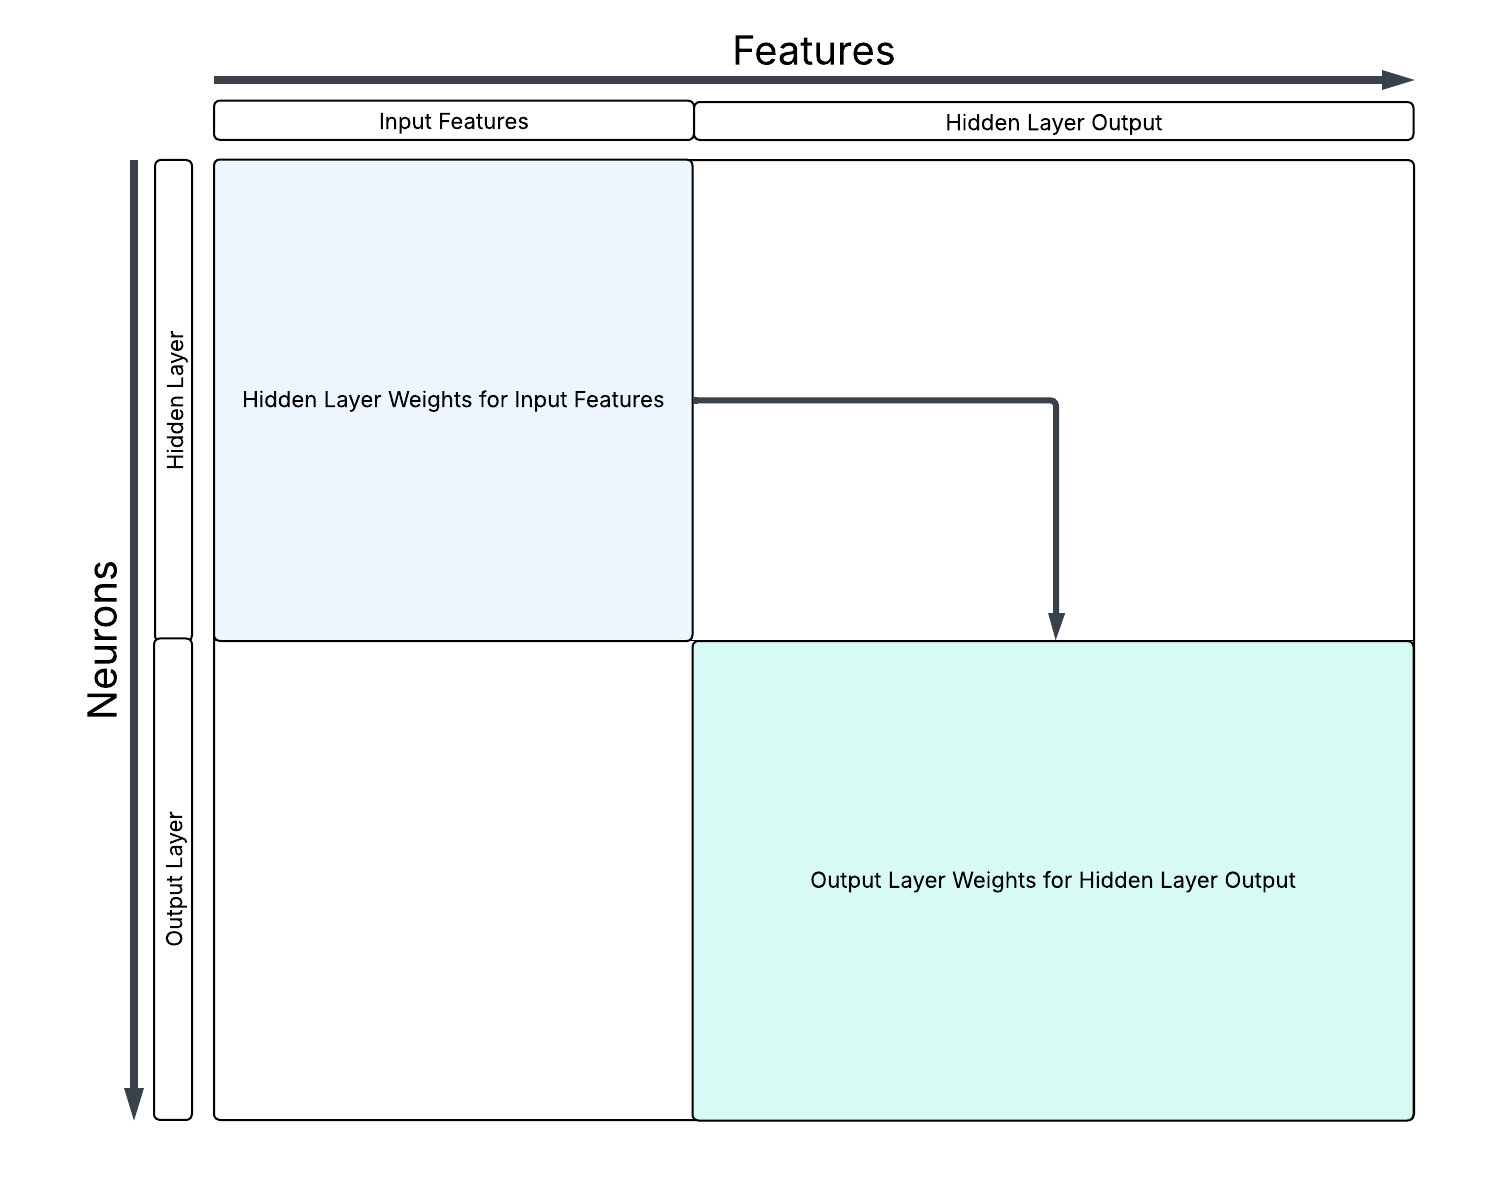
\includegraphics[width=\textwidth]{Figures/Methodology/Minimal_MLP_Weights.png}
        \caption{Minimal MLP.}
        \label{fig:minMLP}
    \end{minipage}%
    \hfill
    \begin{minipage}[t]{0.46\textwidth}
        \centering
        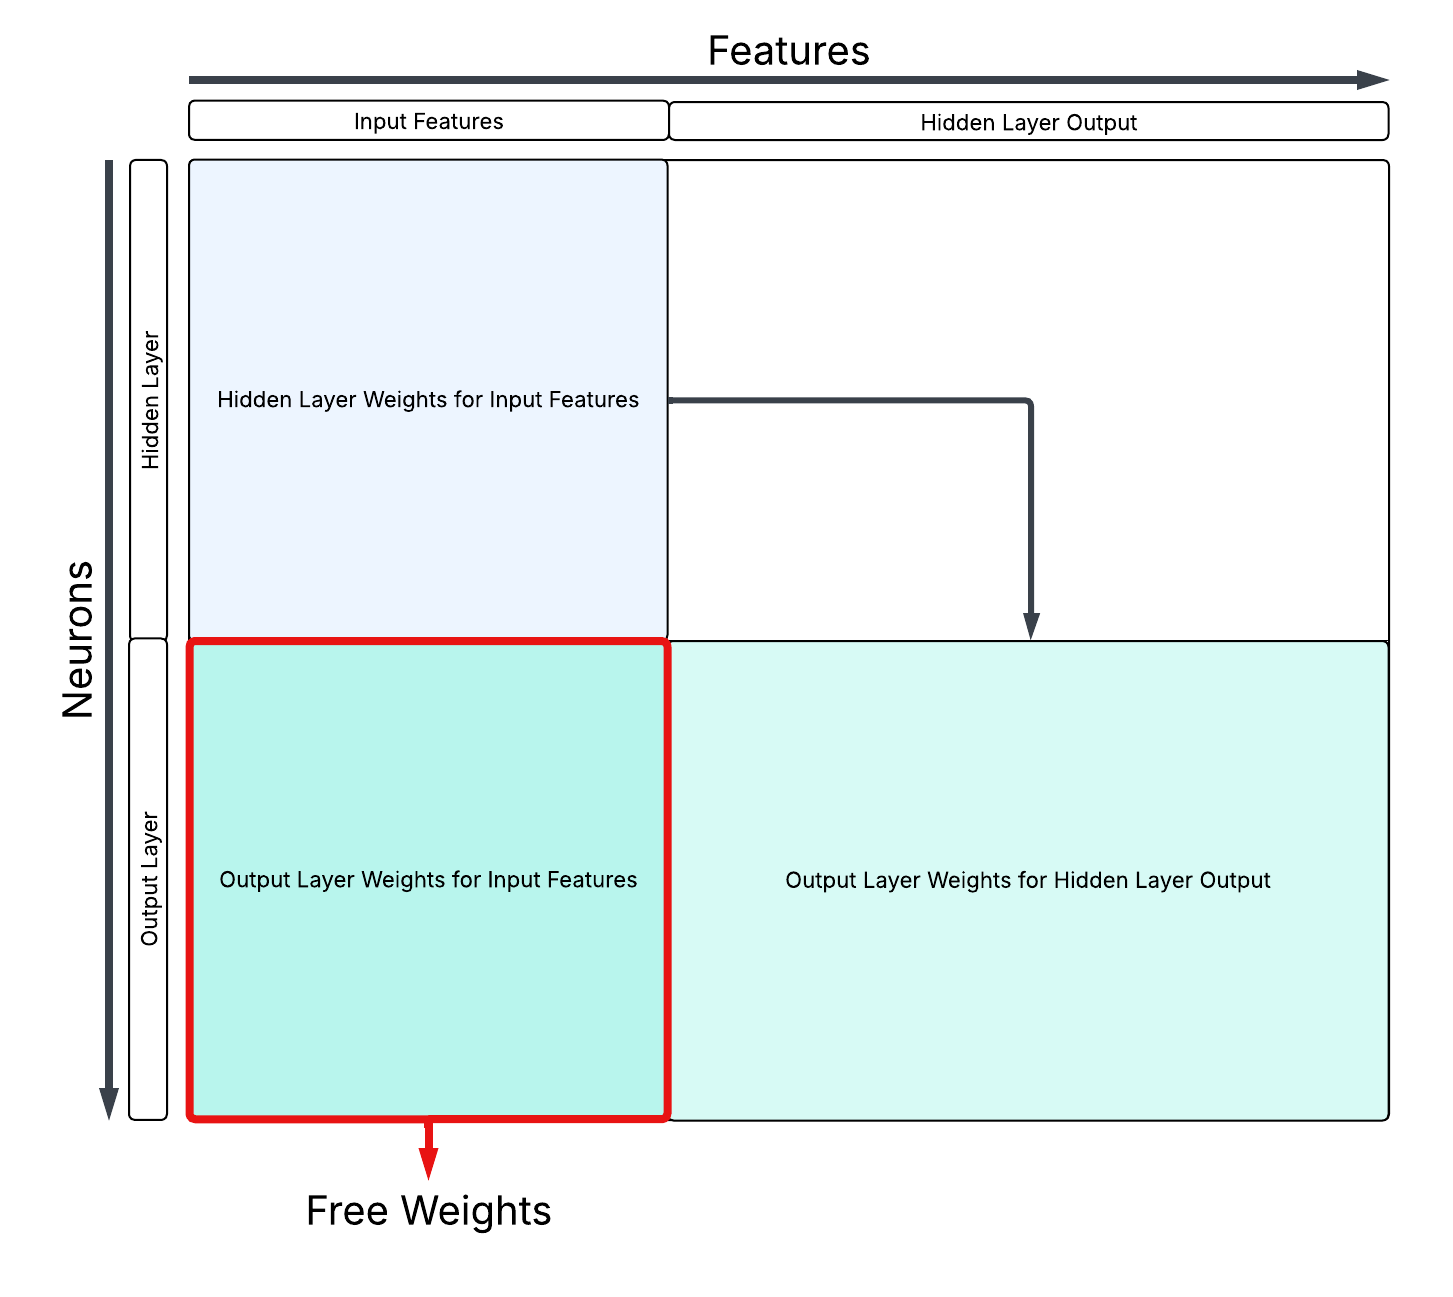
\includegraphics[width=\textwidth]{Figures/Methodology/Minimal_SPN_Weights.png}
        \caption{Minimal SPN.}
        \label{fig:minSpn}
    \end{minipage}
\end{figure}

\section{Implementation Approach}

In practice, there are three potential ways of designing the forward-propagation and backpropagation algorithms for SPNs. For all these approaches, the time and space complexity of implementing Maximal SPNs will be considered as they represent the worst case scenario.

\subsection{Object-based Representation with Partial Inputs}

One potential method to achieve the SPN framework is to have neurons, as independent objects, store partial inputs from sources that have completed their forward pass, while still waiting on outputs from other sources that haven't finished. Once a neuron receives all its necessary inputs, it performs its own forward pass and propagates its output to the subsequent neurons.
 
While this approach is conceptually simple and flexible, it is computationally expensive. Each neuron performs a storage and propagation step for every connection it has, leading to a large amount of redundancy. Even though the forward pass is only a single step once the inputs are complete, a worst-case scenario involves performing $n$ forward passes, where $n$ is the total number of neurons. Additionally, since each neuron stores its partial inputs, the outputs from a single neuron are duplicated for every neuron it propagates to. With each neuron also storing weights for every input, this method doubles the memory used compared to a traditional MLP network.

\begin{itemize}
    \item Time complexity: $\mathcal{O}(n^2)$.
    \item Space complexity: $\mathcal{O}(I \cdot n^2)$.
\end{itemize}

%----------------------------------------------------------------------------------------
%	SECTION 2
%----------------------------------------------------------------------------------------

\subsection{Sequential Representation}

In this approach, we describe the SPN using a list of weights, where every element in the list corresponds to the weights of a single neuron, exactly how it was illustrated in Figure \ref{fig:maxSpn}.
 
Such a network contains all possible connections for a given number of neurons. Therefore, any other network with the same number of neurons is a subnetwork of this complete network. To process this network, neurons are processed sequentially, starting from the first neuron in the list and proceeding to the last. For each step, the output of a neuron is appended to its input, providing the input for the subsequent neuron. By doing so, we eliminate the need to add partial inputs for each neuron individually. Instead, the same input can be compounded across the forward pass.

This approach assumes a maximum connection for every neuron. Disconnecting two neurons is achieved by zeroing out the weight value for the output neuron corresponding to the input. This method resembles traditional MLP pruning, where weight values are zeroed out instead of being removed entirely.

While this method eliminates the propagation step from every neuron to its subsequent neurons, it still requires each neuron to temporarily store its input during the backpropagation process. Therefore, this approach does not reduce space complexity.

\begin{itemize}
    \item Time complexity: $\mathcal{O}(n)$.
    \item Space complexity: $\mathcal{O}(I \cdot n^2)$.
\end{itemize}

\subsection{Block-based Representation}

When considering the weight matrix of a Maximal SPN, we can draw vertical lines at the edge of each neuron’s weight vector, forming vertical blocks within the matrix. The largest block, which is the first block, contains the weights corresponding to the input features, and subsequent blocks contain the weights for the output of each neuron as showin in Figure \ref{fig:blockMaxSpn}.
 
Rather than processing each neuron’s weight vector individually, this approach processes the network one block at a time. The top-most neuron’s forward pass is completed first, followed by calculating partial outputs for the remaining neurons. This method improves the time complexity by prioritizing the heaviest calculations (typically when the hardware is under lower load), and adds slight parallelization, as an input value is accessed only once, rather than repeatedly in a sequential approach.

This method is both energy and time-efficient, offering significant improvements over the previous approaches.

\begin{itemize}
    \item Time complexity: $\mathcal{O}(n)$.
    \item Space complexity: $\mathcal{O}(I \cdot n^2)$.
\end{itemize}

\begin{figure}[h!]
\centering
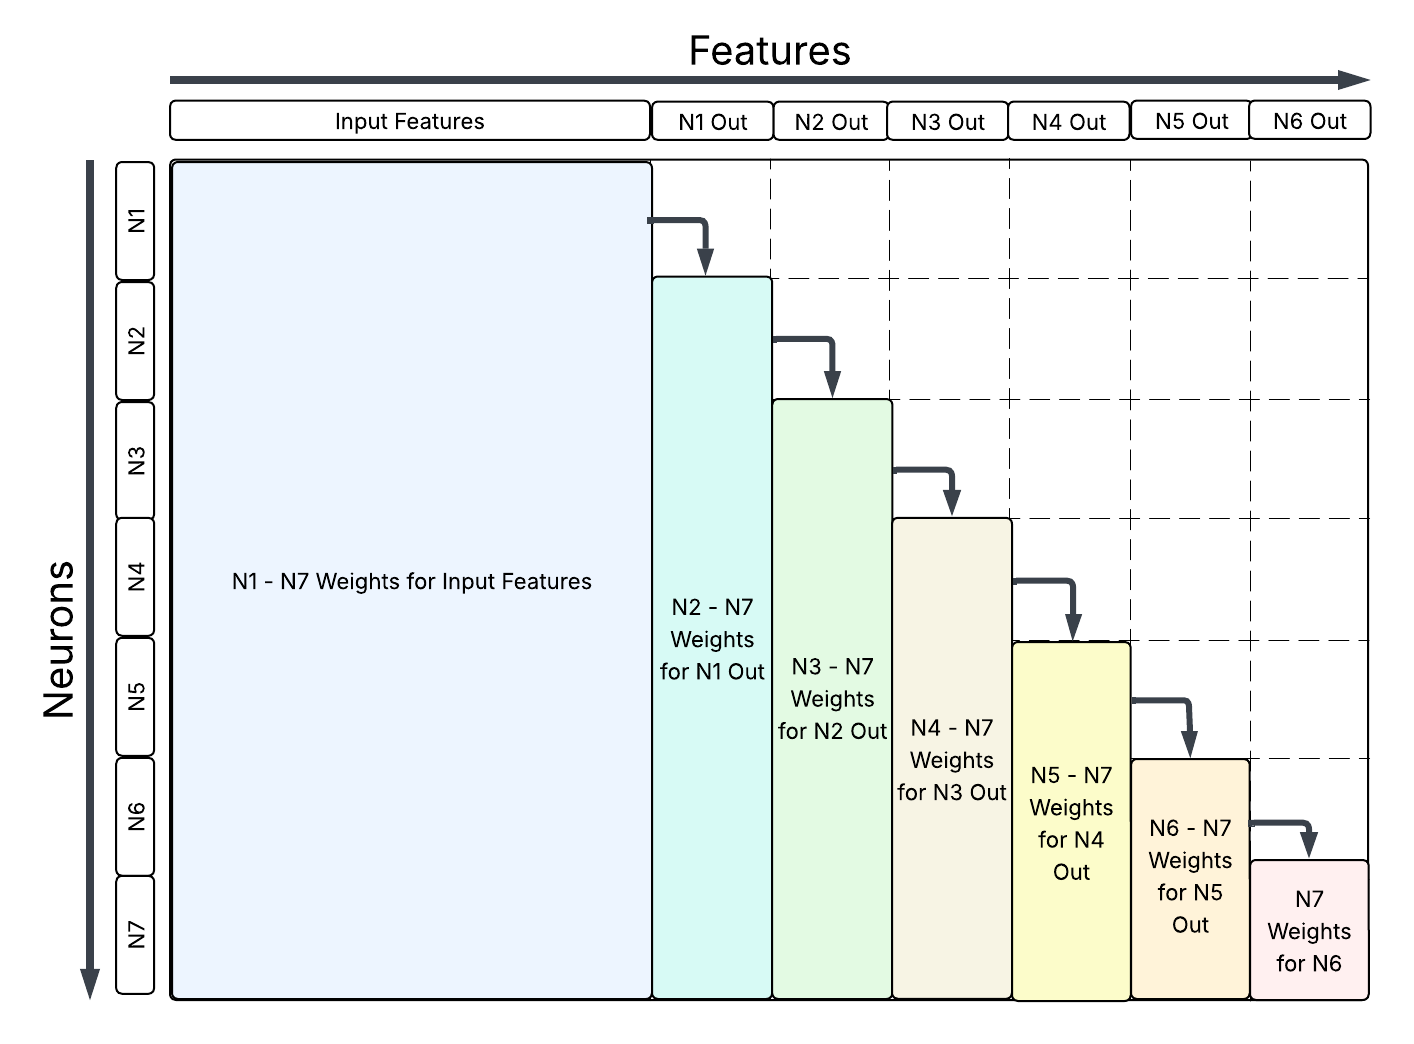
\includegraphics[width=0.8\textwidth]{Figures/Methodology/Block_Based_Maximal_SPN_Weights.png}
\caption{Illustration of a block based Maximal SPN.}
\label{fig:blockMaxSpn}
\end{figure}

\subsection{Summary}

The performance difference between the sequential and block-based approaches is minimal, as both exhibit the same overall time complexity. Their relative efficiency primarily depends on the underlying hardware. The block-based approach front-loads the computational burden by handling the most demanding calculations first, while the sequential approach distributes the workload more evenly across all steps. Depending on the hardware and the specific model architecture, one approach may be preferable over the other.

\begin{table}[h!]
\centering
\caption{Comparison of time and space complexities for the implementation approaches.}
\begin{tabular}{|l|l|l|}
\hline
\textbf{Approach}    & \textbf{Time Complexity} & \textbf{Space Complexity} \\
\hline
Object Based          & $\mathcal{O}(n^2)$        & $\mathcal{O}(I \cdot n^2)$        \\
Sequential          & $\mathcal{O}(n)$        & $\mathcal{O}(I \cdot n^2)$       \\
Block Based              & $\mathcal{O}(n)$        & $\mathcal{O}(I \cdot n^2)$        \\
\hline
\end{tabular}
\label{tab:approachescomplexityComparison}
\end{table}

In this thesis, the sequential method was chosen for its balanced workload distribution; with larger models, the block-based approach could potentially overwhelm hardware resources at the outset, resulting in slower performance. Ultimately, a hybrid strategy that combines elements of both approaches may offer the greatest efficiency.

Overall, this thesis aims to investigate whether introducing cross-layer connections, intra-layer connections, or both can enable MLPs to achieve a deeper understanding of the data and/or improve their computational efficiency. The experimental setup and the corresponding results for that investigation are presented in the subsequent chapters.
% Chapter Template

\chapter{Experiments} % Main chapter title

\label{Experiments} % Change X to a consecutive number; for referencing this chapter elsewhere, use \ref{ChapterX}

%----------------------------------------------------------------------------------------
%	SECTION 1
%----------------------------------------------------------------------------------------

\section{Experimental Setup}

This section provides a detailed description of the experimental environment, datasets, model architectures, evaluation metrics, and procedures used to evaluate Sarosh’s Perceptron Networks (SPNs) in comparison to traditional Multi-Layer Perceptrons (MLPs). These experiments aim to rigorously assess the performance of SPNs across multiple domains; images, tabular data, and language data, and varying complexity levels within each domain.
%-----------------------------------
%	SUBSECTION 1
%-----------------------------------
\subsection{Experimental Environment}
All our experiments were carried out with the following hardware specifications and software environment. Python was used for development. The hardware and software configurations are shown in Table \ref{tab:hardware} and \ref{tab:software} respectively.

\begin{table}[h!]
\centering
\caption{Hardware Specifications.}
\label{tab:hardware}
\begin{tabular}{| m{4cm} | m{6cm} |}
\hline
\textbf{Component} & \textbf{Details} \\
\hline
GPU & NVIDIA Tesla V100-PCIE GPU \\
GPU memory & 16GB \\
\hline
\end{tabular}
\end{table}

\begin{table}[h!]
\centering
\caption{Software Environment.}
\label{tab:software}
\begin{tabular}{| m{4cm} | m{4cm} |}
\hline
\textbf{Component} & \textbf{Version} \\
\hline
Python & 3.9.21 \\
PyTorch & 1.9.0 \\
CUDA & 11.8.0 \\
Transformers & 4.49.0 \\
Tensorflow & 2.10.0 \\
scikit-learn & 1.6.1 \\
Datasets & 3.3.2 \\
Matplotlib & 3.9.4 \\
\hline
\end{tabular}
\end{table}

\subsection{Datasets}

To address \ref{RQ5}, the experiments were structured across three distinct domains: images, tabular data, and language data. For each domain, two datasets were chosen. One, referred to as the simple variant, had fewer input features and training samples, while the complex variant had more. This approach allowed a comprehensive evaluation of SPN performance across varying complexity and data modalities.

For binary classification tasks, the number of classes was set to 2 as it allowed us to use the same optimizer (ADAM) and loss function (CrossEntropy Loss) as the multi-class classification tasks.

\subsubsection{Image Datasets}
For the image domain, the MNIST dataset served as the simpler variant. MNIST consists of 70,000 grayscale images of handwritten digits from 0–9, with 60,000 images allocated for training and 10,000 images reserved for testing. Each image is represented by 784 pixel features. 

The complex image dataset selected was CIFAR-10, which contains 60,000 RGB color images divided evenly into 10 classes—airplane, automobile, bird, cat, deer, dog, frog, horse, ship, and truck. CIFAR-10 is structured into 50,000 training images and 10,000 test images, each with 3,072 pixel features.

\subsubsection{Tabular Datasets}
In the tabular domain, the simple variant chosen was the Titanic dataset, which contains passenger information aimed at predicting survival during the Titanic disaster. Features include passenger class, gender, age, number of siblings or spouses aboard, number of parents or children aboard, fare amount, and embarkation port for a total of 7 input features. The dataset is composed of 712 training samples and 179 test samples, forming a binary classification task.

The complex variant selected was the Covertype dataset, which aims to predict forest cover types based on cartographic variables. The dataset includes 54 features, comprising 14 numerical and 40 binary indicators, representing various wilderness areas and soil types. This dataset contains approximately 88,000 training samples and 22,000 testing samples across 7 forest cover classes.

\subsubsection{Language Datasets}
For text-based tasks, the simple variant was the 20 Newsgroups dataset, comprising approximately 20,000 newsgroup documents categorized into 20 distinct topics such as politics, technology, and sports. The dataset is split into 13,000 training samples and 5,600 testing samples. 

The complex variant was the IMDB Reviews dataset, containing 50,000 movie reviews equally divided into 25,000 training and 25,000 test samples, each labeled with a positive or negative sentiment, making it a binary classification task. Text data in both datasets were standardized to 5,000 features using TF-IDF vectorization.

\subsubsection{Summary}

Across the tabular and language datasets, we selected a combination of simple and complex datasets: the Titanic dataset and the IMDB dataset for binary classification, and the Newsgroups dataset and the Covertype dataset for multi-class classification. This selection allows for a comprehensive evaluation of SPNs and MLPs across binary and multi-class classification tasks of varying complexity. Regression tasks were excluded from these tests to avoid introducing additional variables, ensuring a more focused and reliable comparison between MLPs and SPNs.

Table \ref{tab:dataSummary} outlines a summary of all the datasets used in our experiments.


\begin{table}[h!]
  \centering
    \caption{Dataset Summary.}
   \begin{tabular}{|l|l|l|l|l|l|l|}
    \hline
    \textbf{Name} & \textbf{Domain} & \textbf{Variant} & \textbf{In size} & \textbf{Classes} & \textbf{Train Size} & \textbf{Test Size} \\
    \hline
    MNIST & Image & Simple & 784 & 10 & 60000 & 10000 \\
    CIFAR 10 & Image & Complex & 3072 & 10 & 50000 & 10000 \\
    Titanic & Tabular & Simple & 7 & 2 & 712 & 179 \\
    Covertype & Tabular & Complex & 54 & 7 & 88314 & 22079 \\
    Newsgroups 20 & Language & Simple & 5000 & 20 & 13192 & 5654 \\
    IMDB Reviews & Language & complex & 5000 & 2 & 25000 & 25000 \\
    \hline
  \end{tabular}

  \label{tab:dataSummary}
\end{table}

%-----------------------------------
%	SUBSECTION 2
%-----------------------------------

\subsection{Model Architectures}
The following six model architectures were tested for each dataset. Since the experiments aim to observe the effects of varying levels of connectivity in Perceptron-based models, the total number of neurons were kept consistent throughout the models for each dataset. This ensured that the only variable across each model was their degree of inter-connectivity.

\begin{enumerate}
\item \textbf{Baseline MLP}: A conventional MLP was used as a control benchmark. Preliminary tests revealed that the best-performing MLP models achieved test accuracies exceeding 90\% across most datasets, but required extensive training times, leaving a minimal margin for improvements. Since the primary goal of the experiments was to assess the effects of varying neural connectivity, smaller MLPs that still performed adequately were selected, allowing the potential benefits of SPNs to be more clearly observed.
\item \textbf{Free Weights SPN}: An SPN that mirrors the layer structure of the baseline MLP, but with the addition of free weights; dense skip connections to all preceding layers. This model serves as a modified version of the baseline MLP, specifically designed to address \ref{RQ1}, enabling a direct examination of the effects of increased connection density.
\item \textbf{Mininal SPN}: To address \ref{RQ3}, the minimal SPN is a simplified two-layer architecture designed to maximize throughput while minimizing structural complexity. This model aims to optimize training time and allows us to investigate whether reducing the number of layers in a densely connected SPN can still deliver sufficient performance to justify the trade-off against multi-layer complexity.
\item \textbf{Minimal MLP}: are structurally similar to minimal SPNs, but they lack the denser connectivity inherent to SPNs. This model allows us to explore whether the potential benefits of minimal SPNs are exclusive to that architecture, or if similar advantages can be achieved with a similarly structured MLP. Like the baseline MLP and the Free Weights SPN, the minimal MLP and SPN models provide valuable insights into the distinctions between SPNs and MLPs, helping to address \ref{RQ1}.
\item \textbf{Maximal SPN}: are designed to maximize all connections between perceptrons for a given number of neurons. These models aim to address \ref{RQ2} by determining the upper performance threshold, while fully sacrificing efficiency and training time constraints in the pursuit of accuracy.
\item \textbf{Pruned Maximal SPN}: aim to preserve the performance of Maximal SPNs while optimizing training time. Maximal SPNs undergo a pruning process where zeroed-out weights are eliminated, leading to some neurons being disconnected. These disconnected neurons are subsequently merged into layers, enhancing the time complexity of the model. This approach addresses \ref{RQ6} and allows us to explore the possibility of optimizing maximal MLPs for time efficiency without compromising their higher performance accuracy.
\end{enumerate}


%----------------------------------------------------------------------------------------
%	SECTION 2
%----------------------------------------------------------------------------------------

\section{Experimental Procedure}

Each model was trained systematically over multiple epochs, with training time per epoch, training time per mini batch, average ttraining accuracy, training loss, test accuracy, and test loss recorded at each epoch.

Hyperparameters were fine-tuned through preliminary experimentation to identify optimal learning rates and batch sizes, with the goal of minimizing overfitting while maximizing training efficiency. The final set of hyperparameters enabled a robust comparative analysis across different architectures.

This experimental setup allowed for a comprehensive evaluation of the relative performance and potential advantages of SPNs over traditional MLPs, providing valuable insights across a range of domains and levels of complexity.

\subsection{Metrics}
Model performance on each dataset was evaluated using the following metrics:
\begin{enumerate}
\item \textbf{Parameter Count}: The total number of trainable parameters (weights and biases) in the model. It reflects the internal connectivity of the model.
\item \textbf{Best Test Accuracy}: The highest accuracy achieved on the testing dataset across all epochs.
\item \textbf{Time To Best Test Accuracy}: The cumulative training duration required to reach the epoch where the highest test accuracy was observed.
\item \textbf{Training Efficiency}: The ratio of the best test accuracy to the total training time required to achieve that accuracy. This metric demonstrates how quickly the model reaches its optimal performance and how effective that peak performance is.
\item \textbf{Area Under Curve (AUC) Efficiency}: The area under the test accuracy-time curve, reflecting how rapidly the model achieves high accuracy levels.
\item \textbf{Throughput Efficiency}: The ratio of the best test accuracy achieved to the average training time per epoch. This metric indicates the model's computational throughput and its effectiveness in achieving high performance with that throughput.
\end{enumerate}

In addition to evaluating model performance on each dataset, several other aspects were considered.

\begin{enumerate}
\item \textbf{Baseline MLP architecture}: The architecture for the baseline MLP was described.
\item \textbf{Total Neuron Count}: The total number of neurons (kept consistent across all models) was noted.
\item \textbf{Batch Size and Training Epochs}: Since both metrics can affect training time, they were kept consistent across all models.
\item \textbf{Pruning time for pruned maximal SPNs.}
\item \textbf{Number of layers before and after pruning.}
\item \textbf{Pruning effectiveness}: This was measured as the ratio between the mean epoch time of the max\_spn and the mean epoch time of the pruned\_spn. It reflects how fast the pruned\_spn is compared to the max\_spn.
\end{enumerate}

Together, these metrics enable us to address \ref{RQ4} and perform a comprehensive analysis of SPNs versus MLPs, considering time complexity, space complexity, and performance accuracy. 
% Chapter Template
\chapter{Results} % Main chapter title

\label{Results} % Change X to a consecutive number; for referencing this chapter elsewhere, use \ref{ChapterX}

This chapter presents findings from the experiments conducted to evaluate Sarosh’s Perceptron Networks (SPNs) against traditional Multi-Layer Perceptrons (MLPs), addressing the research questions outlined in Chapter \ref{Introduction}. The results are organized into three sections corresponding to the domains evaluated: Images, Tabular Data, and Text Data. For each domain, results from all model architectures detailed in Chapter \ref{Experiments} are presented, compared, and analyzed.

Throughout this chapter, shorter representations for model names and evaluations have been adopted for clarity:

\begin{table}[h!]
    \centering
    \begin{tabular}{ll}
    \textbf{Full name} & \textbf{Representation used} \\
    \hline
    Models: & \\
    \hspace{1em} Baseline MLP & base\_mlp \\
    \hspace{1em} Free Weights SPN & fw\_spn \\
    \hspace{1em} Minimal SPN & min\_spn \\
    \hspace{1em} Minimal MLP & min\_mlp \\
    \hspace{1em} Maximal SPN & max\_spn \\
    \hspace{1em} Pruned Maximal SPN & pruned\_spn \\
    Evaluation Metrics: & \\
    \hspace{1em} Parameter Count & param\_count \\
    \hspace{1em} Best Test Accuracy & best\_acc \\
    \hspace{1em} Time to Best Accuracy & time\_best \\
    \hspace{1em} Training Efficiency & train\_eff \\
    \hspace{1em} Area Under Curve Efficiency & auc\_eff \\
    \hspace{1em} Throughput Efficiency & thru\_eff \\
    \end{tabular}
\end{table}

%----------------------------------------------------------------------------------------
%	SECTION 1
%----------------------------------------------------------------------------------------

\section{Image Domain Results}

Both image datasets were flattened and normalized before model training.

\subsection{MNIST Dataset}

\begin{tabular}{@{}ll@{}}
\textbf{Variant} & Simple \\
\textbf{Input Features} & 784 \\
\textbf{Output Classes} & 10 \\
\textbf{Batch Size} & 75 \\
\textbf{Training Epochs} & 50 \\
\textbf{Training Samples} & 60,000 \\
\textbf{Test Samples} & 10,000 \\
\textbf{Base MLP Dimensions} & $[12,\, 12,\, 10]$ \\
\textbf{Total Neurons} & 34 \\
\end{tabular}

\begin{figure}[H]
    \centering
    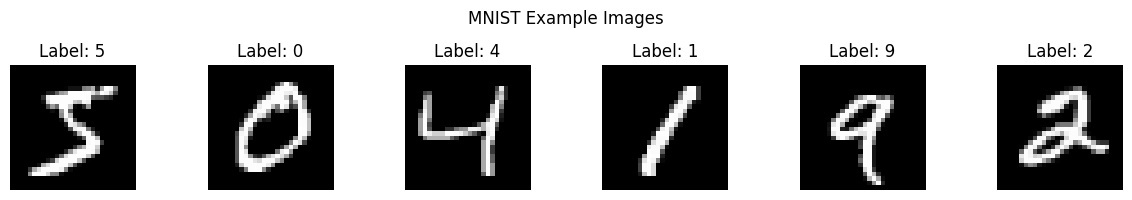
\includegraphics[width=1.0\textwidth]{Figures/Results/MNIST/examples.png} 
    \captionsetup{justification=centering}  % Ensure the caption is centered
    \caption{Example Images in MNIST}
    \label{fig:mnistexamples}
\end{figure}

Preliminary testing showed that very large MLP models could achieve test accuracies approaching those of state-of-the-art models reported on the MNIST leaderboard~\cite{pwc_mnist_leaderboard}, with results nearing 98\%. However, at this level of performance, any improvements offered by SPNs would likely be marginal and difficult to observe. For this reason, a smaller model was chosen as the base MLP to make potential improvements more evident.

\begin{figure}[H]
    \centering
    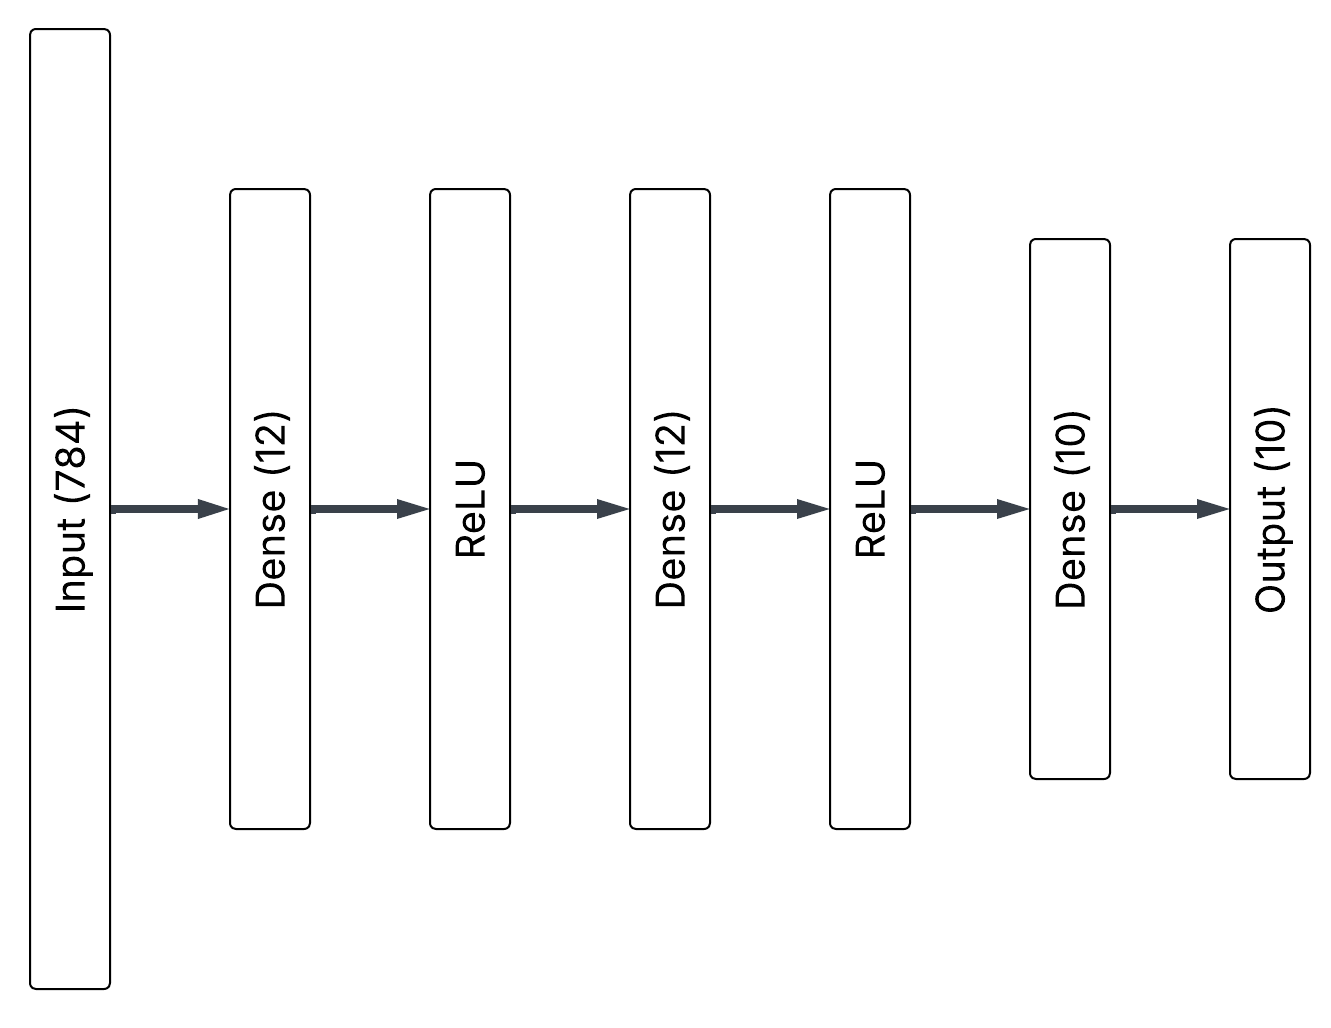
\includegraphics[width=0.6\textwidth]{Figures/Results/MNIST/MNIST_base_mlp_architecture.png} 
    \captionsetup{justification=centering}  % Ensure the caption is centered
    \caption{base\_mlp architecture for MNIST}
    \label{fig:mnistMlpBaseArch}
\end{figure}

The training and testing curves in Figures \ref{fig:mnistTrainCurve} and \ref{fig:mnistTestCurve} clearly demonstrate that the min\_mlp and base\_mlp models underperform relative to all SPN models. Table \ref{tab:mnistResults} offers a detailed comparison of all six models across the efficiency metrics.

\begin{figure}[H]
    \centering
    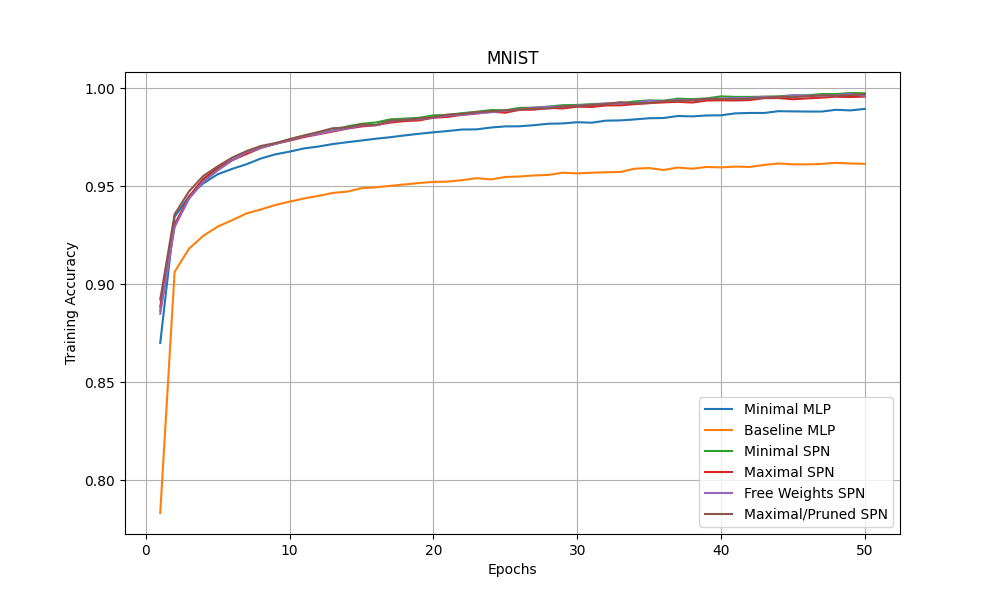
\includegraphics[width=\linewidth]{Figures/Results/MNIST/training_accuracy_plot.png} % first figure itself
    \captionsetup{width=\linewidth}
    \caption{train\_acc vs epochs curve for MNIST}
    \label{fig:mnistTrainCurve}
\end{figure}

\begin{figure}[H]
    \centering
    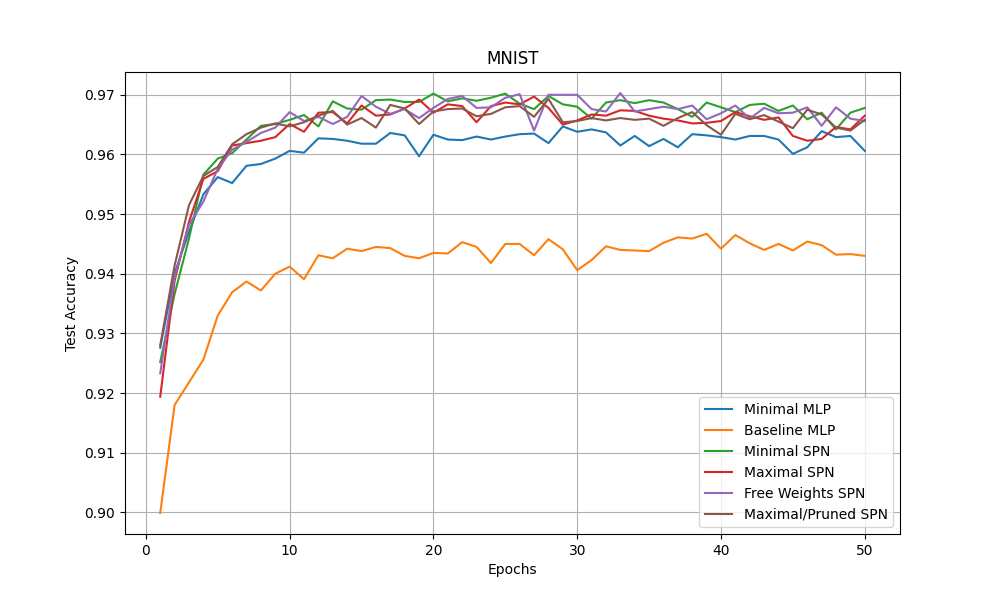
\includegraphics[width=\linewidth]{Figures/Results/MNIST/test_accuracy_plot.png} % second figure itself
    \captionsetup{width=\linewidth}
    \caption{test\_acc vs epochs curve for MNIST}
    \label{fig:mnistTestCurve}
\end{figure}

\begin{table}[h!]
    \centering
    \caption{Cross Model Comparison on the MNIST dataset}
    \begin{tabular}{|l|l|l|l|l|l|l|}
    \hline
    \textbf{Model} & \textbf{param\_count} & \textbf{best\_acc} & \textbf{time\_best} & \textbf{train\_eff} & \textbf{auc\_eff} & \textbf{thru\_eff} \\
    \hline
    base\_mlp & 9,706 & \cellcolor{red!25}94.67\% & 45.34s & 0.021 & \cellcolor{red!25}46.131 & 0.816 \\
    fw\_spn & 27,074  & \cellcolor{green!25}97.03\% & 53.09s  & 0.018 & 47.297 & 0.607 \\
    min\_mlp & 19,090 & 96.47\% & 24.85s & 0.039 & 47.074 & \cellcolor{green!25}1.127 \\
    min\_spn & 26,930 & 97.02\% & \cellcolor{green!25}18.23  & \cellcolor{green!25}0.053 & \cellcolor{green!25}47.318 & 1.043 \\
    max\_spn & 27,251  & 96.97\% & \cellcolor{red!25}399.87s & \cellcolor{red!25}0.002 & 47.246 & \cellcolor{red!25}0.064 \\
    pruned\_spn & 27,025 & 96.93\% & 44.99s & 0.022 & 47.256 & 0.595 \\
    \hline
    \end{tabular}
    \label{tab:mnistResults}
\end{table}

\begin{enumerate}
\item \textbf{Baseline MLP vs. Free Weights SPN}: The fw\_spn model achieved the highest test accuracy, clearly outperforming the base\_mlp, which had the lowest accuracy out of all the models. The notable increase in parameter count of the fw\_spn, while retaining the same layer layout as the base\_mlp, correlates positively with its improved accuracy, providing strong evidence that enhanced internal connectivity boosts model performance. Although fw\_spn had slightly lower training and throughput efficiencies than the base\_mlp, this trade-off was justified by the considerable gain in accuracy.
\item \textbf{Minimal MLP vs. Minimal SPN}: Both min\_spn and min\_mlp achieved better accuracy compared to base\_mlp but slightly lower than fw\_spn. This suggests that having a higher param\_count might be more advantageous in this dataset than having more layers. Min\_spn consistently outperformed min\_mlp across all metrics except throughput efficiency, where both models were fairly close to one another. This further emphasizes the benefit of increased neural connectivity on model performance.
\item \textbf{Maximal SPN}: Max\_spn model had the third-highest accuracy but required significantly longer training times compared to the other models. This suggests a performance ceiling for the MNIST dataset, where additional internal connections yield diminishing returns.
\item \textbf{Pruned SPN}:
\begin{center}  % Centers the table
\begin{tabular}{|l|l|}
\hline
\textbf{Metric} & \textbf{Value} \\
\hline
Layers Before Pruning & 34 \\
Layers After Pruning & 3 \\
Mean Epoch Time Before Pruning & 15.89s \\
Mean Epoch Time After Pruning & 1.59s \\
Pruning Time & 631.68s \\
Pruning Effectiveness & 9.99 \\
\hline
\end{tabular}
\end{center}

The pruned\_spn model achieved accuracy similar to max\_spn while dramatically improving computational efficiency. Although the pruning process itself was time-consuming, taking longer than it took max\_spn to reach its peak accuracy (making it practically unusable), it still made the max\_spn model nearly 10x faster in average training time, validating the efficacy of pruning for optimizing maximal SPNs. Additionally, this pruning confirmed that a three-layer architecture is sufficient for optimal performance on this dataset. 

However, since max\_spn did not outperform any of the other models, it suggests that there was limited additional learning to be done, making pruning easier on this particular dataset.
\end{enumerate}

Overall, SPNs convincingly outperformed their MLP counterparts on the MNIST dataset. Maximal and pruned SPNs confirmed the existence of an upper performance bound, highlighting the effectiveness of strategic pruning to balance accuracy and efficiency.

\subsection{CIFAR 10 Dataset}

\begin{tabular}{@{}ll@{}}
\textbf{Variant} & Complex \\
\textbf{Input Features} & 3072 \\
\textbf{Output Classes} & 10 \\
\textbf{Batch Size} & 128 \\
\textbf{Training Epochs} & 30 \\
\textbf{Training Samples} & 50,000 \\
\textbf{Test Samples} & 10,000 \\
\textbf{Base MLP Dimensions} & $[256,\, 128,\, 64,\, 32,\, 10]$ \\
\textbf{Total Neurons} & 490 \\
\end{tabular}

\begin{figure}[H]
    \centering
    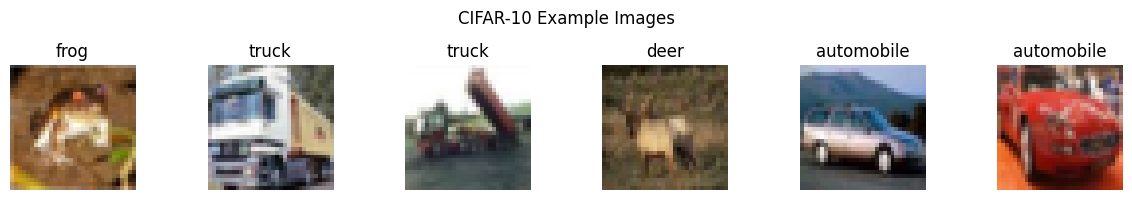
\includegraphics[width=1.0\textwidth]{Figures/Results/CIFAR_10/examples.png} 
    \captionsetup{justification=centering}  % Ensure the caption is centered
    \caption{Example Images in CIFAR 10}
    \label{fig:cifarexamples}
\end{figure}

In preliminary tests on this dataset, all MLP models exhibited clear overfitting. This contrasted with the results on MNIST, likely because MNIST images are much simpler (being grayscale handwritten digits) \ref{fig:mnistexamples}, and the train and test sets are more homogeneous. In CIFAR-10, however, the diversity and complexity of classes \ref{fig:cifarexamples}, as well as the substantial differences between training and test samples, pose challenges that perceptron-based models struggle to overcome. This aligns with observations from the CIFAR-10 leaderboard~\cite{pwc_cifar10_leaderboard}, where the best-performing models are specialized architectures such as Convolutional Neural Networks (CNNs) and Vision Transformers (ViTs).

Although data augmentation and regularization techniques were applied in initial experiments, they did not yield significant improvements. Consequently, this dataset was used to illustrate the upper limits of complexity in image classification and to examine how MLPs and SPNs (both based on perceptron architectures) compare when faced with such challenging data. This dataset also had the largest base\_mlp model among all datasets used in these experiments.

\begin{figure}[H]
    \centering
    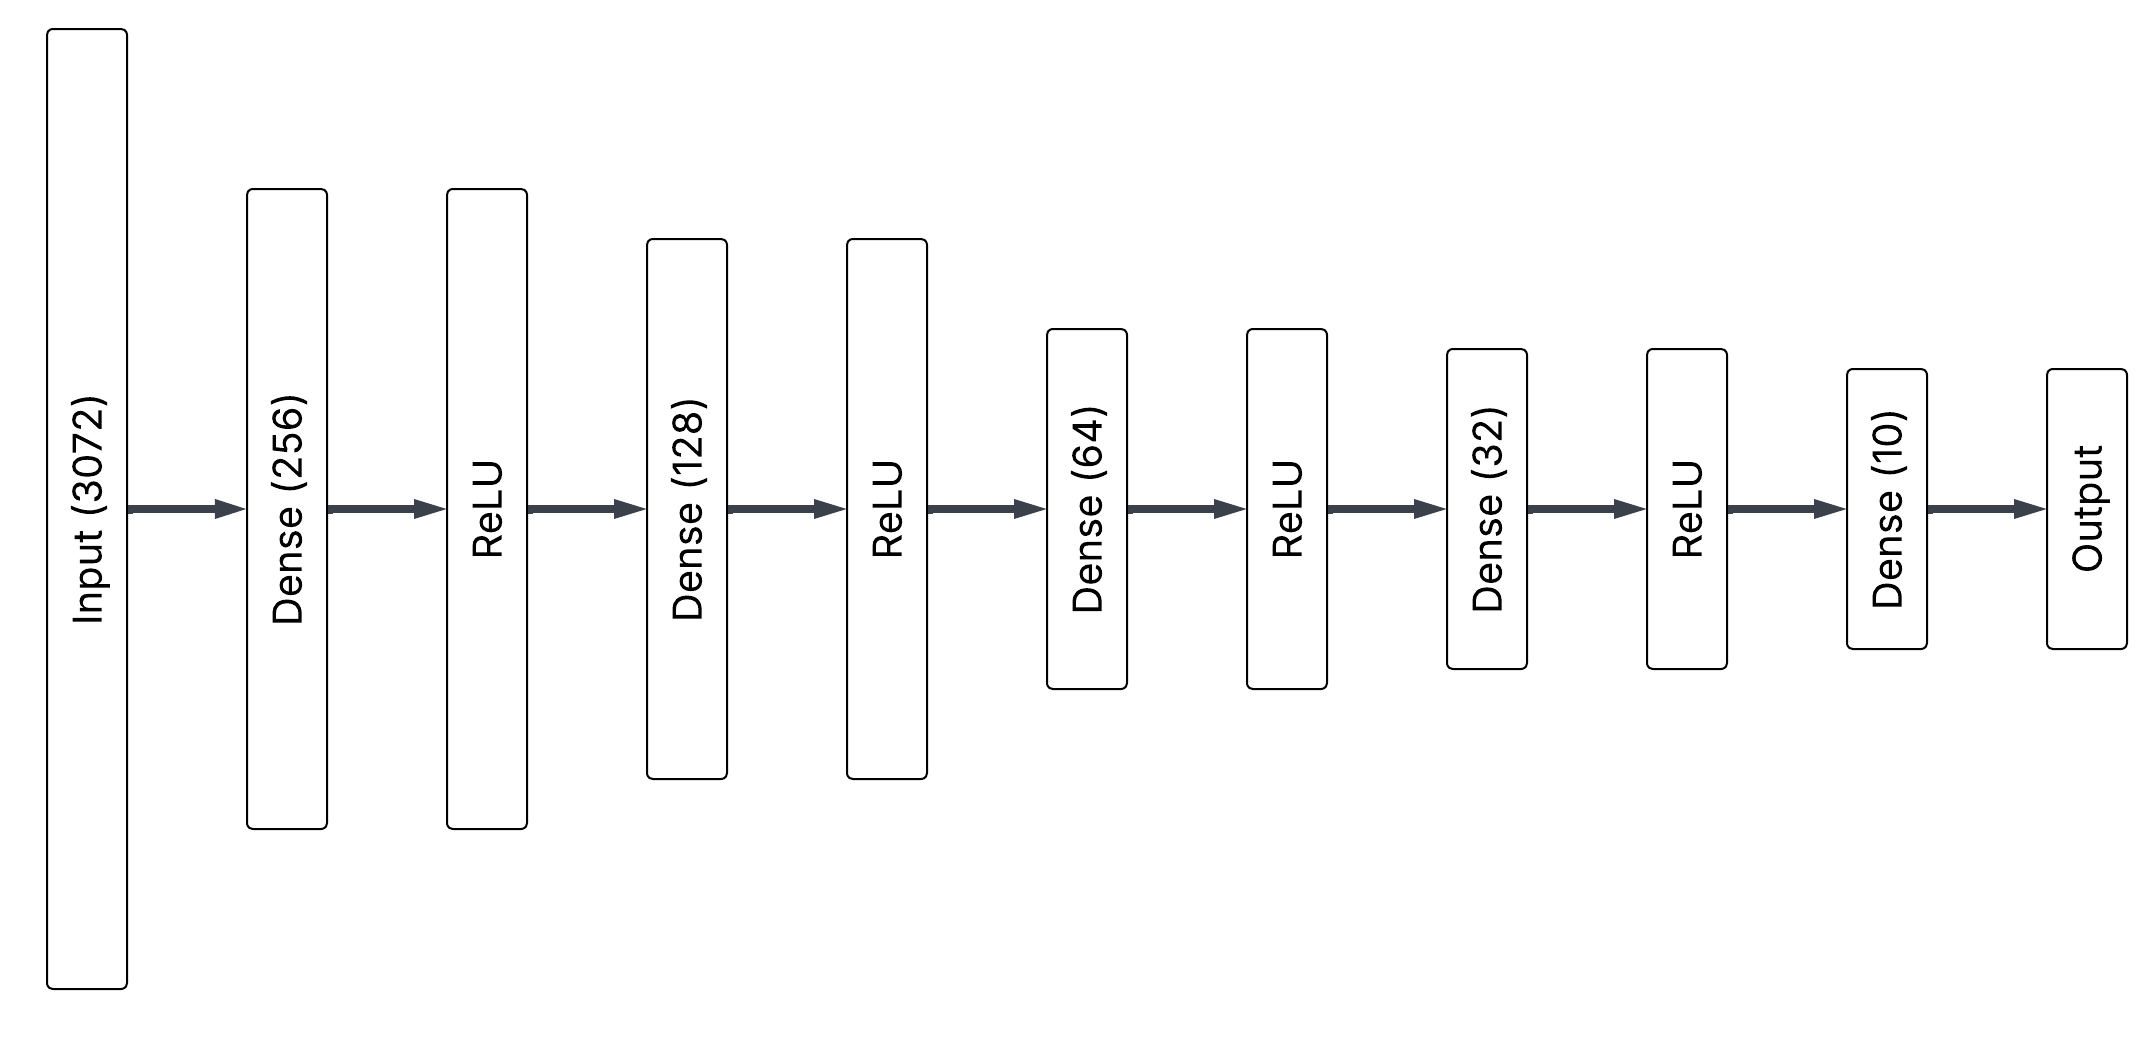
\includegraphics[width=1.0\textwidth]{Figures/Results/CIFAR_10/CIFAR_base_mlp_architecture.png} 
    \captionsetup{justification=centering}  % Ensure the caption is centered
    \caption{base\_mlp architecture for CIFAR 10}
    \label{fig:cifarMlpBaseArch}
\end{figure}

The training curve in Figure \ref{fig:cifarTrainCurve} follows the expected trend: the smaller models (min\_mlp and min\_spn) underperform relative to base\_mlp and fw\_spn, while pruned\_spn and max\_spn achieve the highest training scores. However, the test curve in Figure \ref{fig:cifarTestCurve} reveals that base\_mlp outperforms all other models on unseen data. This indicates that increasing the number of connections may actually worsen generalization in this case, as it encourages overfitting to the training set. Table \ref{tab:cifarResults} provides additional evidence to support this observation.

\begin{figure}[H]
    \centering
    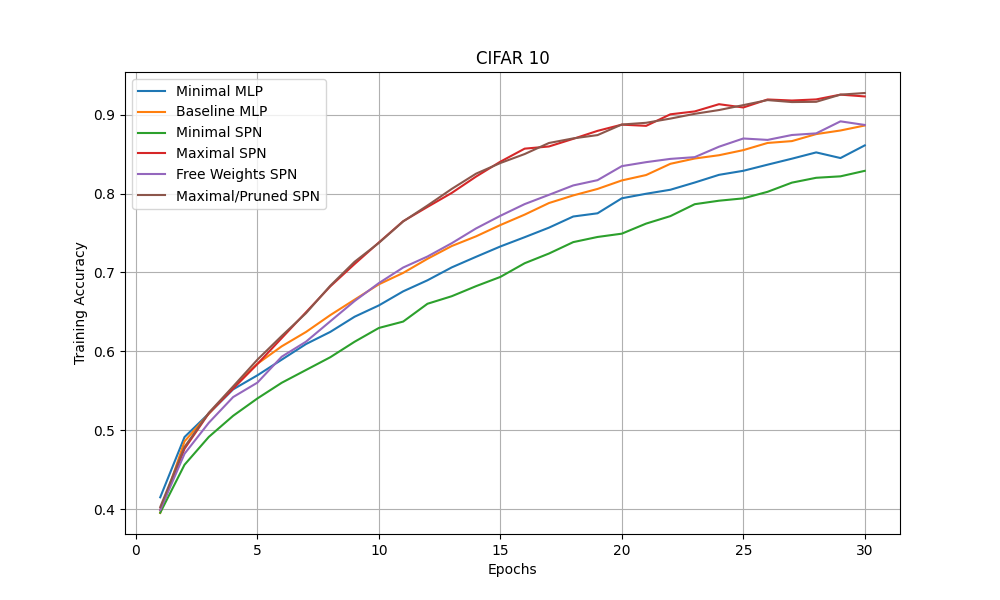
\includegraphics[width=\linewidth]{Figures/Results/CIFAR_10/training_accuracy_plot.png} % first figure itself
    \captionsetup{width=\linewidth}
    \caption{train\_acc vs epochs curve for CIFAR 10}
    \label{fig:cifarTrainCurve}
\end{figure}

\begin{figure}[H]
    \centering
    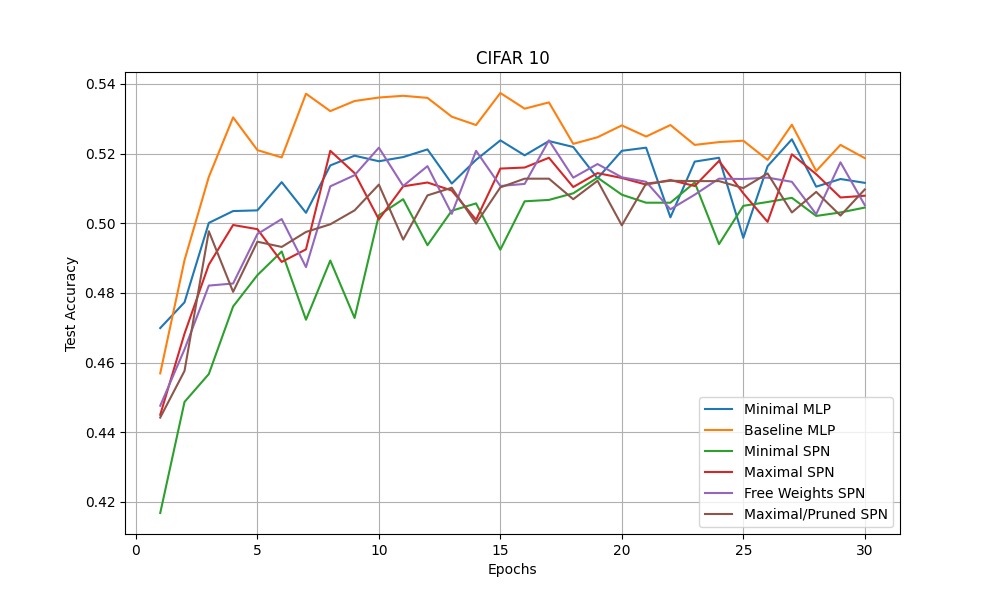
\includegraphics[width=\linewidth]{Figures/Results/CIFAR_10/test_accuracy_plot.png} % second figure itself
    \captionsetup{width=\linewidth}
    \caption{test\_acc vs epochs curve for CIFAR 10}
    \label{fig:cifarTestCurve}
\end{figure}

\begin{table}[h!]
    \centering
    \caption{Cross Model Comparison on the CIFAR 10 Dataset}
    \begin{tabular}{|l|l|l|l|l|l|l|}
    \hline
    \textbf{Model} & \textbf{param\_count} & \textbf{best\_acc} & \textbf{time\_best} & \textbf{train\_eff} & \textbf{auc\_eff} & \textbf{thru\_eff} \\
    \hline
    base\_mlp & 830,250 & \cellcolor{green!25}53.74\% & 14.12s & 0.038 & \cellcolor{green!25}15.220 & 0.585 \\
    fw\_spn & 1,582,250 & 52.38\% & 19.57s & 0.027 & 14.671 & 0.449 \\
    min\_mlp & 1,479,850 & 52.41\% & 12.83s & 0.041 & 14.856 & \cellcolor{green!25}1.100 \\
    min\_spn & 1,510,570 & \cellcolor{red!25}51.31\% & \cellcolor{green!25}10.60s & \cellcolor{green!25}0.048 & \cellcolor{red!25}14.342 & 0.925 \\
    max\_spn & 1,625,575 & 52.08\% & \cellcolor{red!25}472.26s & \cellcolor{red!25}0.001 & 14.672 & \cellcolor{red!25}0.009 \\
    pruned\_spn & 1,623,931 & 51.43\% & 453.08s & \cellcolor{red!25}0.001 & 14.567 & 0.029 \\
    \hline
    \end{tabular}
    \label{tab:cifarResults}
\end{table}

\begin{enumerate}
\item \textbf{Baseline MLP vs. Free Weights SPN}: The base\_mlp achieved the highest test accuracy, with the fw\_spn following closely behind. Additionally, base\_mlp demonstrated greater efficiency than fw\_spn, further underscoring the limitations of increasing internal connectivity in perceptron-based models. In complex datasets like CIFAR 10, where spatial relationships are lost during flattening, increasing connections primarily leads to greater overfitting rather than better generalization, making the less-connected base\_mlp the better choice.
\item \textbf{Minimal MLP vs. Minimal SPN}: A similar trend was observed with the smaller models, min\_mlp attained the second-highest test accuracy and overall efficiency, while min\_spn recorded the lowest test accuracy. This further supports the conclusion that, in scenarios prone to overfitting, additional connections can degrade model performance.
\item \textbf{Maximal SPN}: The max\_spn model achieved only moderate test accuracy, indicating that increasing model depth or complexity does not translate to improved results for perceptron-based models on CIFAR-10. This suggests that such architectures are inherently limited in capturing the complex relationships present in image data.
\item \textbf{Pruned SPN}:
\begin{center}  % Centers the table
\begin{tabular}{|l|l|}
\hline
\textbf{Metric} & \textbf{Value} \\
\hline
Layers Before Pruning & 34 \\
Layers After Pruning & 86 \\
Mean Epoch Time Before Pruning & 62.06s \\
Mean Epoch Time After Pruning & 17.85s \\
Pruning Time & 1520.61s \\
Pruning Effectiveness & 3.48 \\
\hline
\end{tabular}
\end{center}

Although the pruned\_spn improved the throughput of max\_spn, it did not offer meaningful gains in training or AUC efficiency. Since max\_spn itself was not a strong performer, improving its speed offers little practical value. Moreover, the pruning process took significantly longer than the best\_time for max\_spn, highlighting inefficiencies in the pruning algorithm and the need for further optimization.

\end{enumerate}

Overall, this experiment highlighted the limitations of perceptron-based models when applied to complex image data. SPNs did not provide any meaningful improvements on such datasets; in fact, their increased internal connectivity exacerbated the overfitting already observed in traditional MLPs, ultimately leading to even poorer generalization performance.

\section{Tabular Domain Results}

For these datasets, pre-processing involved filling missing values, encoding categorical variables and removing unncessary features.

\subsection{Titanic Dataset}

\begin{tabular}{@{}ll@{}}
\textbf{Variant} & Simple \\
\textbf{Input Features} & 7 \\
\textbf{Output Classes} & 2 \\
\textbf{Batch Size} & 32 \\
\textbf{Training Epochs} & 50 \\
\textbf{Training Samples} & 712 \\
\textbf{Test Samples} & 179 \\
\textbf{Base MLP Dimensions} & $[16,\, 8,\, 4,\, 2]$ \\
\textbf{Total Neurons} & 30 \\
\end{tabular}

\vspace{2pt}

During pre-processing, missing values in the 'Age' and 'Embarked' fields were imputed using the median age and the most frequent embarkation point, respectively. The 'Sex' field was converted to a binary variable, while the 'Embarked' field was encoded numerically. The 'Name', 'Ticket', 'Cabin', and 'PassengerId' fields were removed, as they were not relevant for predicting passenger survival. Finally, the 'Survived' column was separated as the target variable.

In early testing, MLP models of various sizes exhibited similar test performance, suggesting that the dataset’s information content may be limited and not further exploitable by increasing model size, especially given the small training set. Consequently, a compact base\_mlp model was chosen to represent traditional MLP performance on such small datasets.

\begin{figure}[H]
    \centering
    \includegraphics[height=0.28\textheight,width=0.7\textwidth]{Figures/Results/Titanic/titanic_base_mlp_architecture.png} 
    \captionsetup{justification=centering}  % Ensure the caption is centered
    \caption{base\_mlp architecture for Titanic}
    \label{fig:titanicMlpBaseArch}
\end{figure}

The training and test curves in Figures \ref{fig:titanicTrainCurve} and \ref{fig:titanicTestCurve} indicate that all models quickly converge to their optimal performance, with no single model standing out as clearly superior or inferior. Given that the best accuracy achieved across all six models in table \ref{tab:titanicResults} is one of two values, and the small sizes of both the training and test sets, this strongly suggests that additional data would be necessary to capture any subtle patterns within the dataset, and that increasing model connectivity through SPNs alone offers little benefit in this context.

\begin{figure}[H]
    \centering
    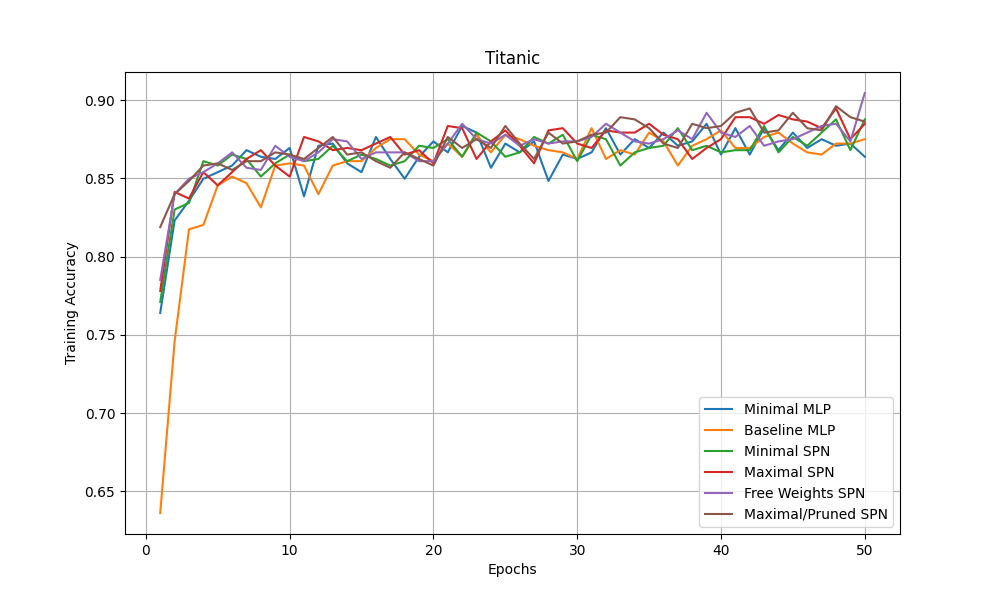
\includegraphics[width=\linewidth]{Figures/Results/Titanic/training_accuracy_plot.png} % first figure itself
    \captionsetup{width=\linewidth}
    \caption{train\_acc vs epochs curve for Titanic}
    \label{fig:titanicTrainCurve}
\end{figure}

\begin{figure}[H]
    \centering
    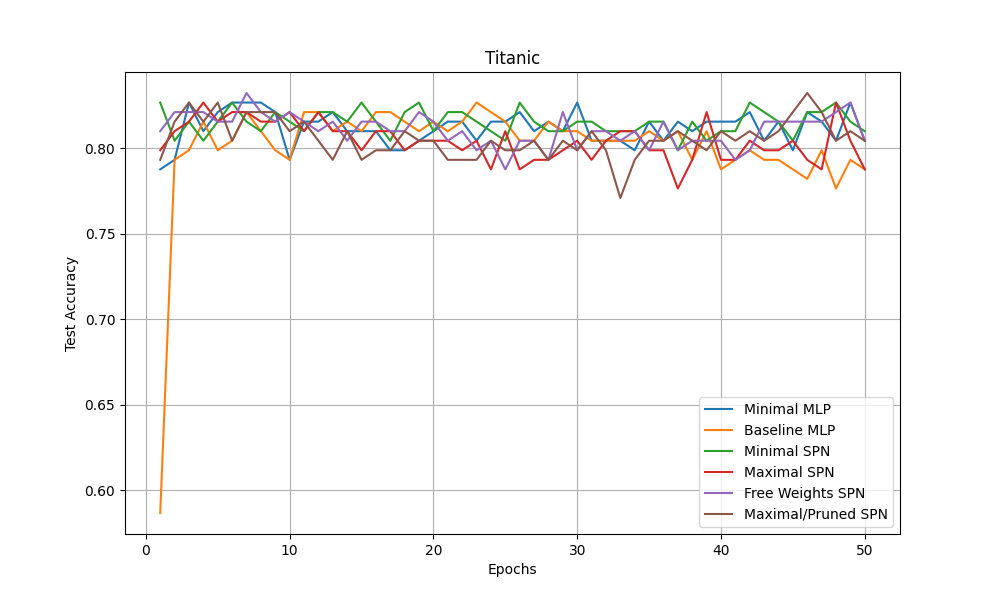
\includegraphics[width=\linewidth]{Figures/Results/Titanic/test_accuracy_plot.png} % second figure itself
    \captionsetup{width=\linewidth}
    \caption{test\_acc vs epochs curve for Titanic}
    \label{fig:titanicTestCurve}
\end{figure}

\begin{table}[h!]
    \centering
    \caption{Titanic Dataset results}
    \begin{tabular}{|l|l|l|l|l|l|l|}
    \hline
    \textbf{Model} & \textbf{param\_count} & \textbf{best\_acc} & \textbf{time\_best} & \textbf{train\_eff} & \textbf{auc\_eff} & \textbf{thru\_eff} \\
    \hline
    base\_mlp & 310 & \cellcolor{red!25}82.68\% & 0.86s & 0.960 & \cellcolor{red!25}39.369 & 22.032 \\
    fw\_spn & 520 & \cellcolor{green!25}83.24\% & 0.33s & 2.560 & 39.735 & 18.331 \\
    min\_mlp & 282 & \cellcolor{red!25}82.68\% & 0.09s & 9.020 & 39.802 & \cellcolor{green!25}36.282 \\
    min\_spn & 296 & \cellcolor{red!25}82.68\% & \cellcolor{green!25}0.02s & \cellcolor{green!25}34.747 & \cellcolor{green!25}39.941 & 33.714 \\
    max\_spn & 675 & \cellcolor{red!25}82.68\% & 1.72s & 0.482 & 39.430 & \cellcolor{red!25}2.376 \\
    pruned\_spn & 655 & \cellcolor{green!25}83.24\% & \cellcolor{red!25}8.05s & \cellcolor{red!25}0.103 & 39.503 & 4.746 \\
    \hline
    \end{tabular}
    \label{tab:titanicResults}
\end{table}

\begin{enumerate}
\item \textbf{Baseline MLP vs. Free Weights SPN}: Although all models performed similarly overall, the fw\_spn outperformed the base\_mlp in every metric except throughput efficiency. However, the slight reduction in throughput is easily justified by the fw\_spn’s higher accuracy, as well as its significantly better training efficiency and AUC efficiency scores.
\item \textbf{Minimal MLP vs. Minimal SPN}: While both small models achieved similar test accuracy, the min\_spn surpassed the min\_mlp and all other models in training efficiency. Although min\_mlp demonstrated higher throughput efficiency, potentially making it more suitable for practical deployment, the superior training and AUC efficiency of min\_spn make it a preferable choice for evaluating performance on small datasets for testing and research purposes.
\item \textbf{Maximal SPN}: As with the MNIST and CIFAR-10 datasets, the max\_spn did not demonstrate any significant performance gains and exhibited poor efficiency scores. This further highlights that increasing the layer count in perceptron-based models yields little to no benefit, particularly when working with small datasets.
\item \textbf{Pruned SPN}:
\begin{center}  % Centers the table
\begin{tabular}{|l|l|}
\hline
\textbf{Metric} & \textbf{Value} \\
\hline
Layers Before Pruning & 30 \\
Layers After Pruning & 15 \\
Mean Epoch Time Before Pruning & 0.32s \\
Mean Epoch Time After Pruning & 0.18s \\
Pruning Time & 1.65s \\
Pruning Effectiveness & 1.78 \\
\hline
\end{tabular}
\end{center}
The pruned\_spn was arguably the weakest performer in this test, recording the lowest training efficiency and the worst time to best test accuracy. Moreover, the pruning process took as long as it did for max\_spn to reach its best accuracy. Altogether, these results indicate that pruning offered no meaningful benefit for such a small dataset.

\end{enumerate}

Overall, the small dataset size limited our ability to observe strong evidence that increased connectivity improves performance on tabular data. However, the fact that the SPN counterparts consistently outperformed their MLP equivalents provides a promising indication of the potential benefits of enhanced connectivity.

\subsection{Covertype Dataset}

\begin{tabular}{@{}ll@{}}
\textbf{Variant} & Complex \\
\textbf{Input Features} & 54 \\
\textbf{Output Classes} & 7 \\
\textbf{Batch Size} & 256 \\
\textbf{Training Epochs} & 150 \\
\textbf{Training Samples} & 88,314 \\
\textbf{Test Samples} & 22,079 \\
\textbf{Base MLP Dimensions} & $[128,\, 64,\, 7]$ \\
\textbf{Total Neurons} & 199 \\
\end{tabular}

For preprocessing, the numeric columns were normalized, and the categorical features for soil types 1–40 were encoded as binary variables.

Early testing revealed that bigger MLPs achieved competitive accuracy on this dataset, comparable to the results reported on the leaderboards~\cite{kaggle_covertype_leaderboard}. And since the test accuracy was closer to 80\%, a three-layer MLP of substantial size was selected for further experiments as there was signifcant room for observing improvements, if any were made by using SPN techniques.

\begin{figure}[H]
    \centering
    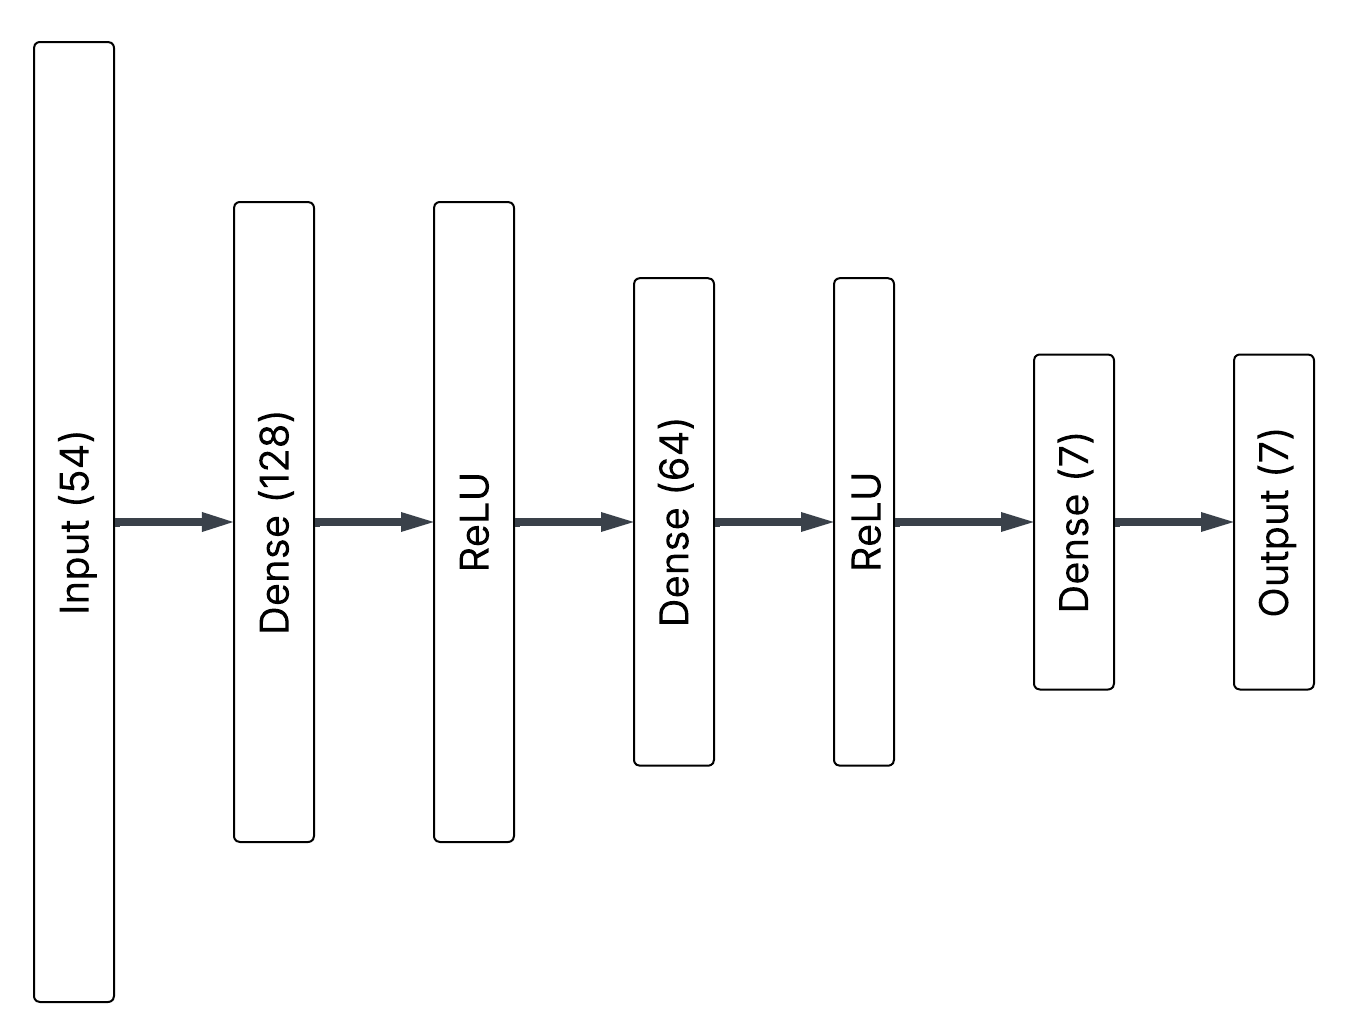
\includegraphics[height=0.28\textheight,width=0.6\textwidth]{Figures/Results/Covertype/Covertype_base_mlp_architecture.png} 
    \captionsetup{justification=centering}  % Ensure the caption is centered
    \caption{base\_mlp architecture for Covertype}
    \label{fig:covertypeMlpBaseArch}
\end{figure}

The training and testing curves in Figures \ref{fig:covertypeTrainCurve} and \ref{fig:covertyoeTestCurve} closely align with theoretical expectations for these models. The results cluster into three distinct tiers: min\_spn and min\_mlp perform at the lowest level, fw\_spn and base\_mlp occupy the middle, and pruned\_spn and max\_spn achieve the highest performance. Within these groupings, SPNs consistently outperform their MLP equivalents. These findings clearly demonstrate that increasing the number of connections in MLP models, as implemented in SPNs, leads to improved model performance and data representation. Moreover, the results underscore that perceptron-based architectures are particularly well-suited to tabular data with well-defined features, as opposed to image data, where individual pixel values carry little standalone meaning.

\begin{figure}[H]
    \centering
    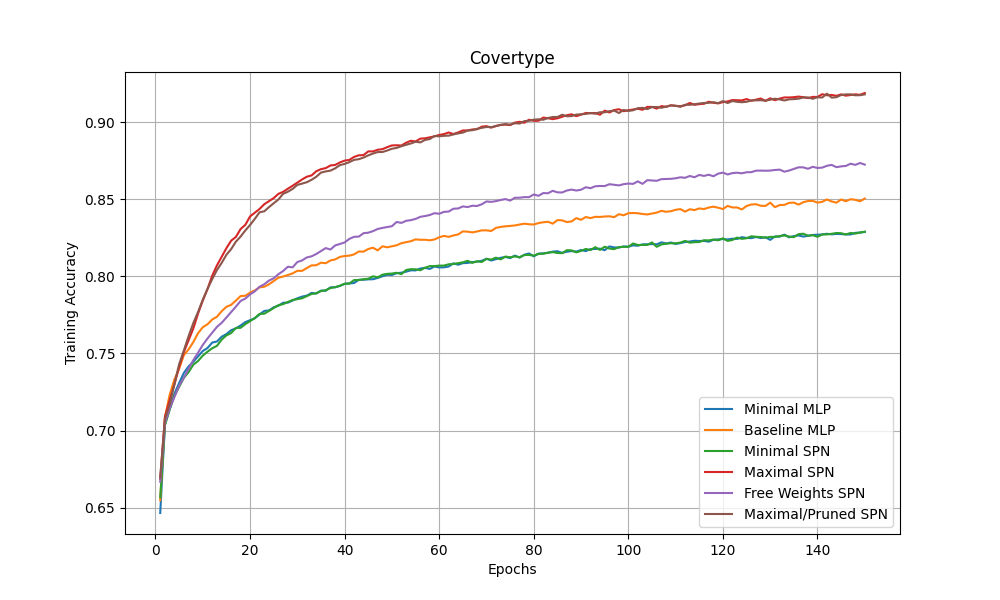
\includegraphics[width=\linewidth]{Figures/Results/Covertype/training_accuracy_plot.png} % first figure itself
    \captionsetup{width=\linewidth}
    \caption{train\_acc vs epochs curve for Covertype}
    \label{fig:covertypeTrainCurve}
\end{figure}

\begin{figure}[H]
    \centering
    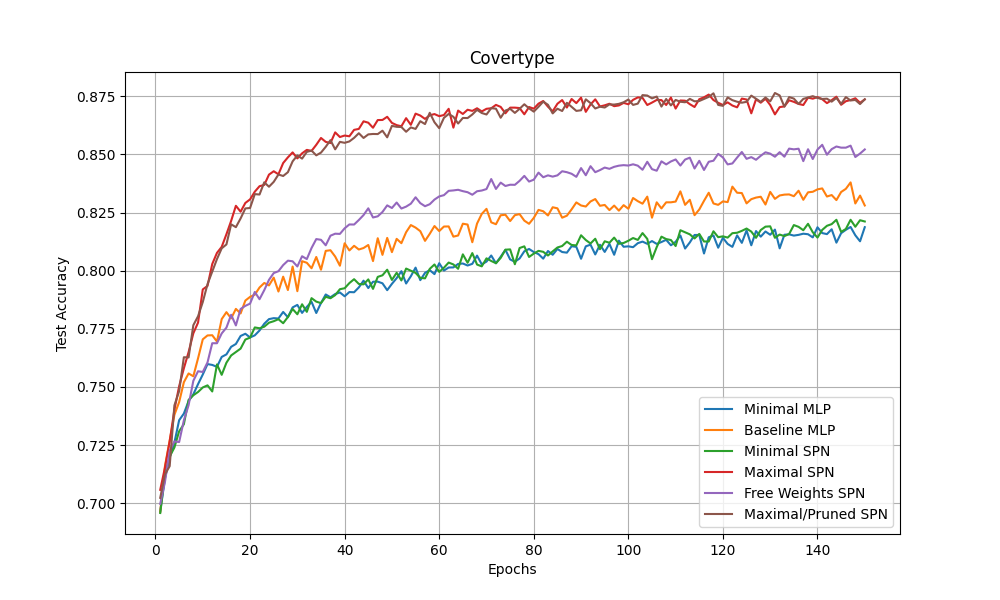
\includegraphics[width=\linewidth]{Figures/Results/Covertype/test_accuracy_plot.png} % second figure itself
    \captionsetup{width=\linewidth}
    \caption{test\_acc vs epochs curve for Covertype}
    \label{fig:covertyoeTestCurve}
\end{figure}

\begin{table}[h!]
    \centering
    \caption{Covertype Dataset results}
    \begin{tabular}{|l|l|l|l|l|l|l|}
    \hline
    \textbf{Model} & \textbf{param\_count} & \textbf{best\_acc} & \textbf{time\_best} & \textbf{train\_eff} & \textbf{auc\_eff} & \textbf{thru\_eff} \\
    \hline
    base\_mlp & 15,751 & 83.79\% & 64.17s & 0.013 & 121.207 & 1.920 \\
    fw\_spn & 20,481 & 85.41\% & 77.07s & 0.011 & 122.954 & 1.554 \\
    min\_mlp & 11,911 & \cellcolor{red!25}81.88\% & \cellcolor{green!25}48.05s & \cellcolor{green!25}0.017 & \cellcolor{red!25}118.777 & \cellcolor{green!25}2.505 \\
    min\_spn & 12,289 & 82.19\% & 50.29s & 0.016 & 118.906 & 2.354 \\
    max\_spn & 30,646 & 87.57\% & \cellcolor{red!25}2430.20s & \cellcolor{red!25}0.0003 & \cellcolor{green!25}127.573 & \cellcolor{red!25}0.042 \\
    pruned\_spn & 30,520 & \cellcolor{green!25}87.64\% & 2082.85s & 0.0004 & 127.413 & 0.055 \\
    \hline
    \end{tabular}
    \label{tab:covertypeResults}
\end{table}

\begin{enumerate}
\item \textbf{Baseline MLP vs. Free Weights SPN}: The fw\_spn model clearly outperforms the base\_mlp in both best accuracy and AUC efficiency, with only a slight reduction in training efficiency. While base\_mlp does achieve better throughput efficiency, this advantage is unlikely to be significant unless the models are deployed in scenarios involving extremely large data volumes.
\item \textbf{Minimal MLP vs. Minimal SPN}: A similar pattern emerges among the minimal models: min\_spn achieves higher accuracy than min\_mlp, with near identical efficiency scores for both. Although min\_mlp boasts the best training and throughput efficiency of all models, its poor accuracy and AUC efficiency make it unusable in a practical scenario.
\item \textbf{Maximal SPN}: The max\_spn model maintains its pattern of poor efficiency but distinguishes itself by achieving a significantly higher peak test accuracy, surpassing even the third-highest accuracy reported on the Covertype dataset leaderboard~\cite{kaggle_covertype_leaderboard}. Additionally, it achieves the best AUC efficiency score, demonstrating that combining maximal layers with extensive connections can lead to rapid and robust performance on this dataset. This approach also highlights the potential upper limit of model performance given the neuron count, making it valuable during the research and development phase for benchmarking what is achievable.
\item \textbf{Pruned SPN}:
\begin{center}  % Centers the table
\begin{tabular}{|l|l|}
\hline
\textbf{Metric} & \textbf{Value} \\
\hline
Layers Before Pruning & 199 \\
Layers After Pruning & 105 \\
Mean Epoch Time Before Pruning & 20.39s \\
Mean Epoch Time After Pruning & 15.66s \\
Pruning Time & 293.63s \\
Pruning Effectiveness & 1.30 \\
\hline
\end{tabular}
\end{center}

The pruning algorithm operates relatively quickly in this case, saving about a minute of training time compared to max\_spn. However, the improvement in throughput is modest and does not significantly enhance overall efficiency. Notably, pruning does lead to a slight increase in peak test accuracy, resulting in the highest test accuracy among all models. This demonstrates that pruning can positively affect not only throughput but also model performance in some instances.

\end{enumerate}

Overall, this dataset most clearly demonstrated the potential of SPNs, with SPN models consistently outperforming their MLP counterparts. The top-performing SPN even achieved results that are highly competitive with state-of-the-art models on this dataset.

\section{Language Domain Results}

For this domain, the data was vectorized using a TF-IDF vectorizer with English stop words removed and a feature size limited to 5,000.

\subsection{Newsgroups 20 Dataset}

\begin{tabular}{@{}ll@{}}
\textbf{Variant} & Simple \\
\textbf{Input Features} & 5000 \\
\textbf{Output Classes} & 20 \\
\textbf{Batch Size} & 64 \\
\textbf{Training Epochs} & 50 \\
\textbf{Training Samples} & 13,192 \\
\textbf{Test Samples} & 5,654 \\
\textbf{Base MLP Dimensions} & $[16,\, 8,\, 20]$ \\
\textbf{Total Neurons} & 44 \\
\end{tabular}

\vspace{2pt}
In early testing, most MLP architectures demonstrated similar performance on this dataset, achieving strong results quickly. This is likely due to the relatively small size of the 20 Newsgroups dataset, which limits the amount of information available for the models to learn. Consequently, to avoid overfitting, a small MLP model was chosen as the baseline.

\begin{figure}[H]
    \centering
    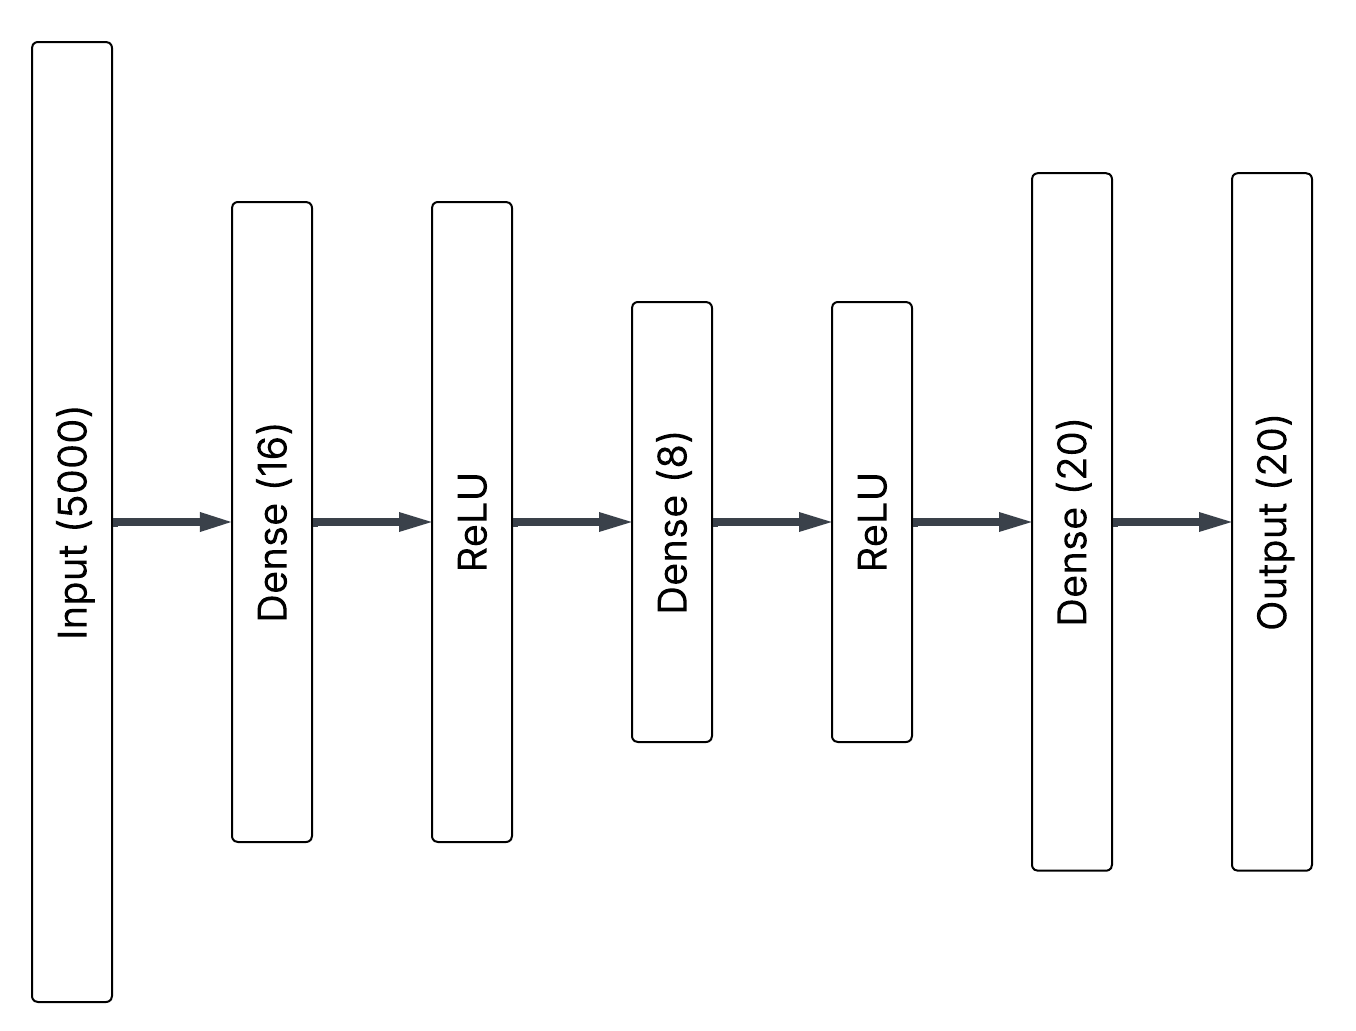
\includegraphics[height=0.28\textheight,width=0.6\textwidth]{Figures/Results/Newsgroups/Newsgroups_base_mlp_architecture.png} 
    \captionsetup{justification=centering}  % Ensure the caption is centered
    \caption{base\_mlp architecture for Newsgroups 20}
    \label{fig:newsgroupsMlpBaseArch}
\end{figure}

The training curves in Figure \ref{fig:newsgroupsTrainCurve} are nearly identical for all models, with the exception of base\_mlp, which converges slightly more slowly. Nevertheless, all models ultimately achieve 100\% training accuracy. In contrast, the test curve in Figure \ref{fig:newsgroupsTestCurve} reveals a clear stratification: the minimal models perform best, followed by fw\_spn, max\_spn, and pruned\_spn, while base\_mlp lags behind. This pattern closely mirrors the results observed in the MNIST experiment.

\begin{figure}[H]
    \centering
    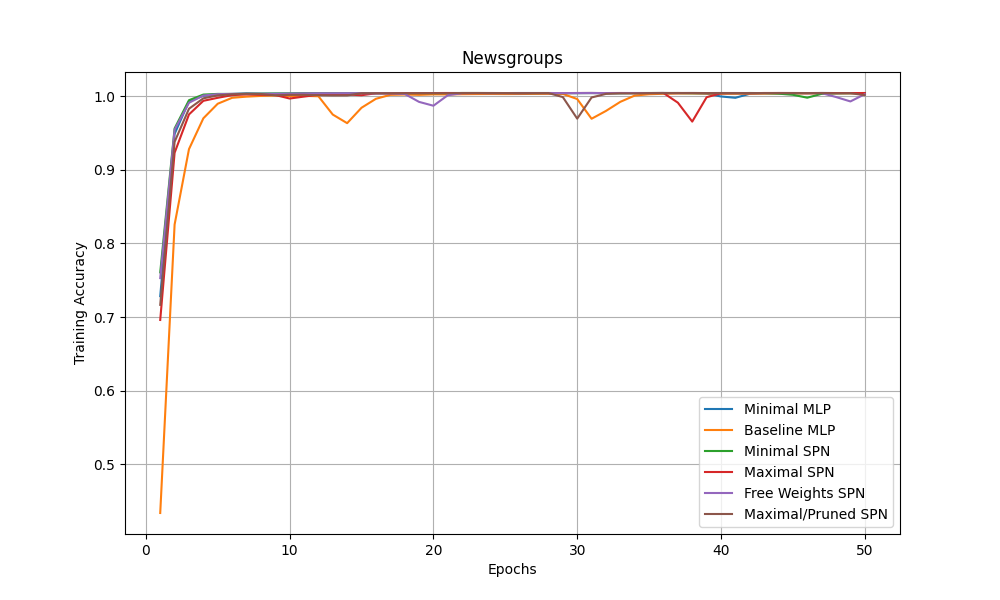
\includegraphics[width=\linewidth]{Figures/Results/Newsgroups/training_accuracy_plot.png} % first figure itself
    \captionsetup{width=\linewidth}
    \caption{train\_acc vs epochs curve for Newsgroups 20}
    \label{fig:newsgroupsTrainCurve}
\end{figure}

\begin{figure}[H]
    \centering
    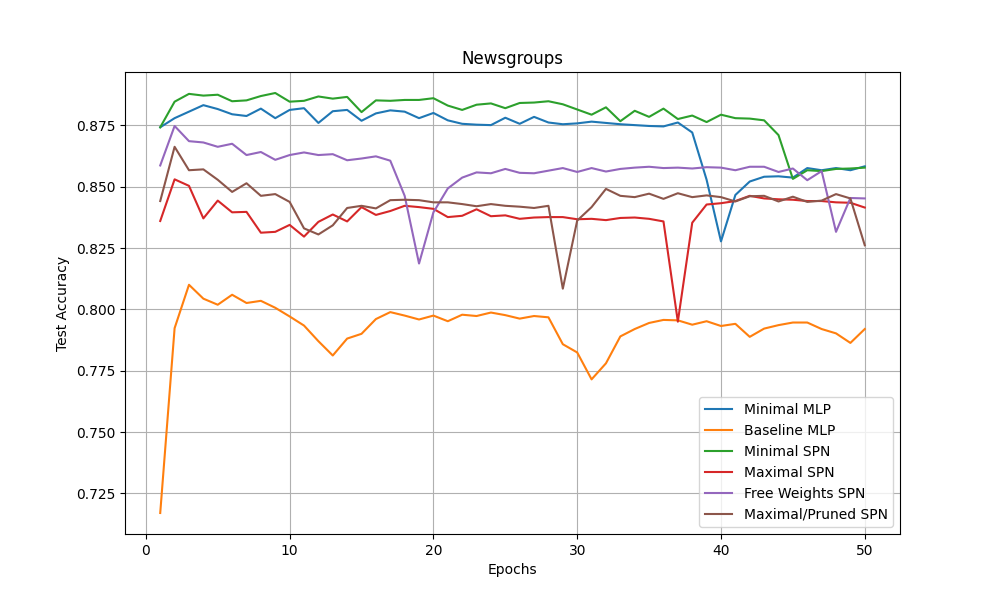
\includegraphics[width=\linewidth]{Figures/Results/Newsgroups/test_accuracy_plot.png} % second figure itself
    \captionsetup{width=\linewidth}
    \caption{test\_acc vs epochs curve for Newsgroups 20}
    \label{fig:newsgroupsTestCurve}
\end{figure}

\begin{table}[h!]
    \centering
    \caption{Newsgroups 20 Dataset results}
    \begin{tabular}{|l|l|l|l|l|l|l|}
    \hline
    \textbf{Model} & \textbf{param\_count} & \textbf{best\_acc} & \textbf{time\_best} & \textbf{train\_eff} & \textbf{auc\_eff} & \textbf{thru\_eff} \\
    \hline
    base\_mlp & 80,332 & \cellcolor{red!25}81.00\% & 0.77s & 1.054 & \cellcolor{red!25}38.869 & 2.938 \\
    fw\_spn & 220,652 & 87.48\% & \cellcolor{green!25}0.64s & \cellcolor{green!25}1.371 & 41.990 & 2.757 \\
    min\_mlp & 120,524 & 88.33\% & 0.91s & 0.967 & 42.720 & 3.937 \\
    min\_spn & 220,524 & \cellcolor{green!25}88.82\% & 2.14s & 0.415 & \cellcolor{green!25}43.105 & \cellcolor{green!25}4.270 \\
    max\_spn & 220,990 & 85.30\% & \cellcolor{red!25}7.99s & \cellcolor{red!25}0.107 & 41.103 & \cellcolor{red!25}0.217 \\
    pruned\_spn & 220,834 & 86.63\% & 1.39s & 0.625 & 41.356 & 1.265 \\
    \hline
    \end{tabular}
    \label{tab:newsgroupsResults}
\end{table}

\begin{enumerate}
\item \textbf{Baseline MLP vs. Free Weights SPN}: This experiment exhibited the largest gap in test accuracy between base\_mlp and the other models, as well as one of the most pronounced differences in parameter count. These findings provide strong evidence that increasing the number of connections can substantially improve performance on certain types of data. Notably, fw\_spn not only outperformed base\_mlp by a significant margin but also achieved the highest training efficiency in this test, making it particularly well-suited for research applications.
\item \textbf{Minimal MLP vs. Minimal SPN}: Surprisingly, the minimal models achieved the highest test accuracy in this experiment. Which suggests that having more layers might be disadvantageous for this kind of data. The min\_spn model, in particular, attained the third-highest test accuracy on the 20 Newsgroups leaderboard~\cite{pwc_20newsgroups_leaderboard}. Combined with its top scores in both AUC efficiency and throughput efficiency, min\_spn stands out as the best-performing model for this dataset among all those tested, making it the clear choice for practical applications.

Min\_mlp also performed well, ranking second in AUC efficiency, throughput efficiency, and test accuracy, but with min\_spn’s outstanding results, the competition was decisively one-sided.
\item \textbf{Maximal SPN}: Unexpectedly, max\_spn produced the second lowest test accuracy while continuing its trend of poor efficiency. This outcome reinforces that increasing model depth does not benefit this type of data; in fact, simpler models might be better suited to capturing the information present in vectorized text.
\item \textbf{Pruned SPN}:
\begin{center}  % Centers the table
\begin{tabular}{|l|l|}
\hline
\textbf{Metric} & \textbf{Value} \\
\hline
Layers Before Pruning & 24 \\
Layers After Pruning & 7 \\
Mean Epoch Time Before Pruning & 3.87s \\
Mean Epoch Time After Pruning & 0.69s \\
Pruning Time & 70.55s \\
Pruning Effectiveness & 5.61 \\
\hline
\end{tabular}
\end{center}

While pruned\_spn outperforms max\_spn across all metrics, its pruning time is nearly ten times longer than the time required for max\_spn to reach its best accuracy. Given the already poor performance of max\_spn, this excessive pruning time renders the process impractical.

\end{enumerate}

Overall, this dataset proved to be the most interesting so far. It was the first instance where the minimal models outperformed their more complex, deeper counterparts. At the same time, the benefits of increased connectivity were clearly demonstrated, with both min\_spn and fw\_spn surpassing their respective MLP counterparts. These results suggest that SPNs may not only enhance performance but also provide insights into the optimal layer complexity and connection density needed for a given dataset.

\subsection{IMDB Reviews Dataset}

\begin{tabular}{@{}ll@{}}
\textbf{Variant} & Complex \\
\textbf{Input Features} & 5000 \\
\textbf{Output Classes} & 2 \\
\textbf{Batch Size} & 32 \\
\textbf{Training Epochs} & 50 \\
\textbf{Training Samples} & 25,000 \\
\textbf{Test Samples} & 25,000 \\
\textbf{Base MLP Dimensions} & $[64,\, 32,\, 2]$ \\
\textbf{Total Neurons} & 96 \\
\end{tabular}

\vspace{2pt}
Preliminary tests on this dataset revealed overfitting issues similar to those observed with CIFAR-10, while also demonstrating that models achieved strong performance early in training, as seen with 20 Newsgroups. Despite this, the best test accuracies were above 80\%, leaving considerable room for improvement through SPNs. Therefore, a mid-sized, three-layer MLP was selected as the baseline for further comparison.

\begin{figure}[H]
    \centering
    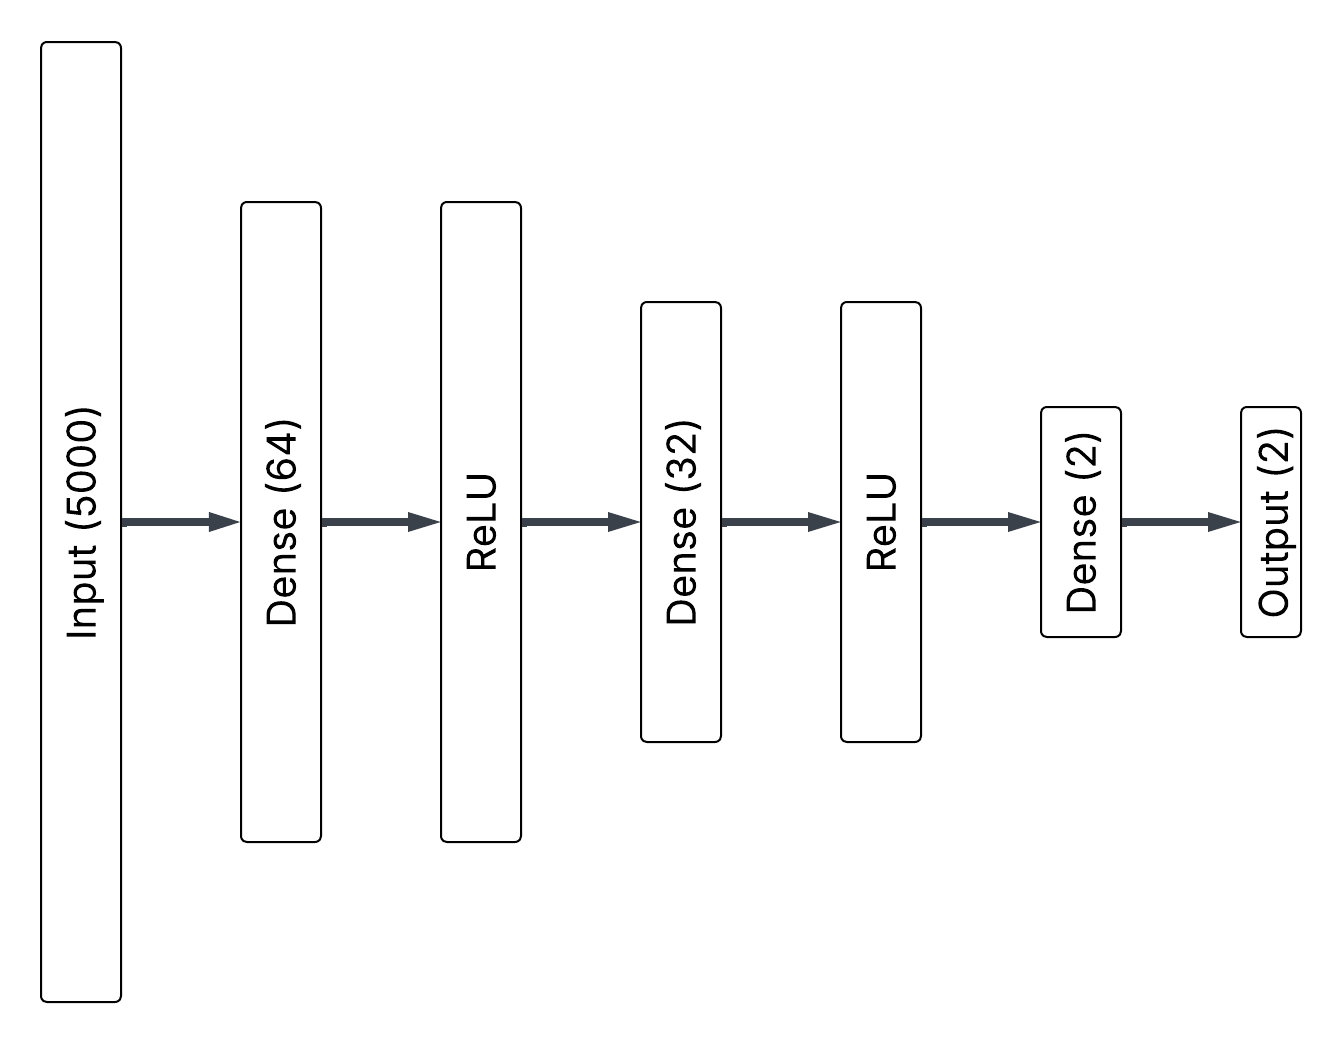
\includegraphics[height=0.28\textheight,width=0.6\textwidth]{Figures/Results/IMDB/IMDB_base_mlp_architecture.png} 
    \captionsetup{justification=centering}  % Ensure the caption is centered
    \caption{base\_mlp architecture for IMDB Reviews}
    \label{fig:imdbMlpBaseArch}
\end{figure}

The training curve in Figure \ref{fig:imdbTrainCurve} closely resembles that of the Newsgroups dataset in Figure \ref{fig:newsgroupsTrainCurve}. However, the test curve in Figure \ref{fig:imdbTestCurve} reveals a steady decline in accuracy as training progresses, indicating pronounced overfitting. This suggests that perceptron-based models may struggle with more complex text tasks, such as sentiment analysis, compared to simpler classification problems.

\begin{figure}[H]
    \centering
    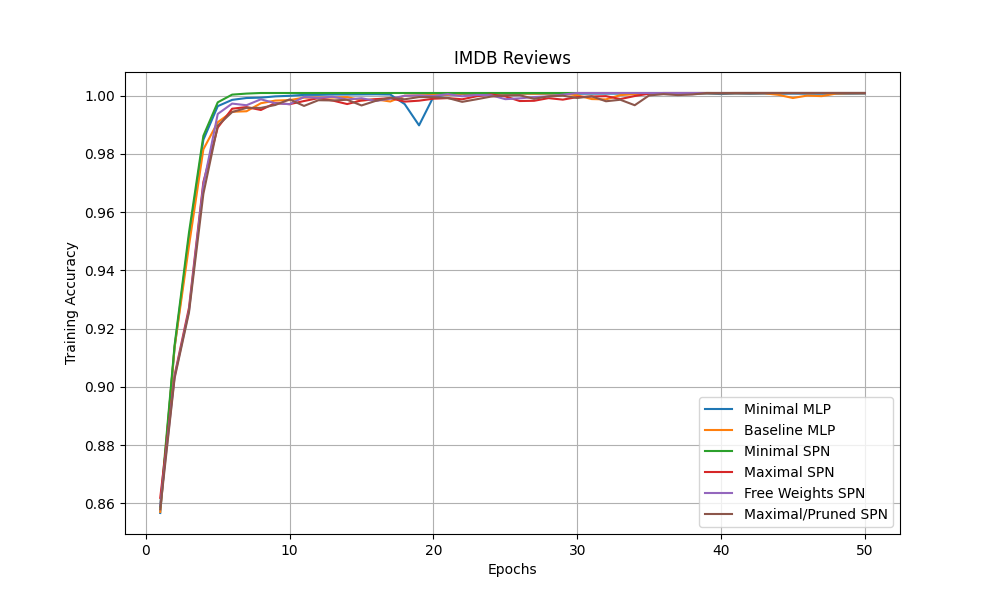
\includegraphics[width=\linewidth]{Figures/Results/IMDB/training_accuracy_plot.png} % first figure itself
    \captionsetup{width=\linewidth}
    \caption{train\_acc vs epochs curve for IMDB Reviews}
    \label{fig:imdbTrainCurve}
\end{figure}

\begin{figure}[H]
    \centering
    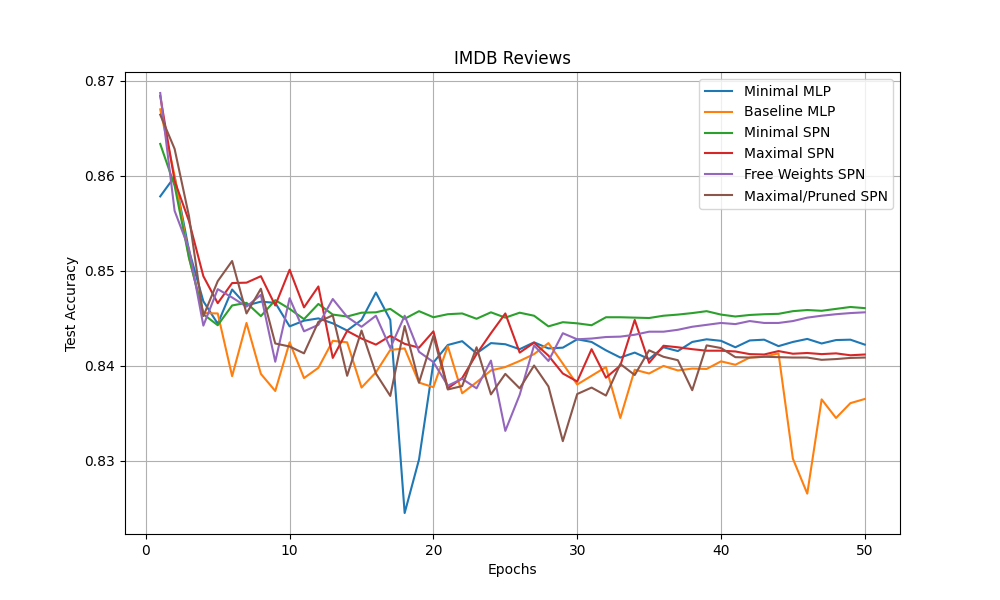
\includegraphics[width=\linewidth]{Figures/Results/IMDB/test_accuracy_plot.png} % second figure itself
    \captionsetup{width=\linewidth}
    \caption{test\_acc vs epochs curve for IMDB Reviews}
    \label{fig:imdbTestCurve}
\end{figure}

\begin{table}[h!]
    \centering
    \caption{IMDB Reviews Dataset results}
    \begin{tabular}{|l|l|l|l|l|l|l|}
    \hline
    \textbf{Model} & \textbf{param\_count} & \textbf{best\_acc} & \textbf{time\_best} & \textbf{train\_eff} & \textbf{auc\_eff} & \textbf{thru\_eff} \\
    \hline
    base\_mlp & 322,210 & 86.70\% & 1.09s & 0.792 & \cellcolor{red!25}41.175 & 0.787 \\
    fw\_spn & 492,338 & \cellcolor{green!25}86.87\% & 1.53s & 0.569 & 41.360 & 0.550 \\
    min\_mlp & 480,290 & \cellcolor{red!25}85.99\% & 1.85s & 0.466 & 41.319 & \cellcolor{green!25}1.009 \\
    min\_spn & 490,290 & 86.34\% & \cellcolor{green!25}0.90s & \cellcolor{green!25}0.955 & \cellcolor{green!25}41.455 & 0.954 \\
    max\_spn & 494,851 & 86.84\% & \cellcolor{red!25}35.29s & \cellcolor{red!25}0.025 & 41.340 & \cellcolor{red!25}0.025 \\
    pruned\_spn & 494,810 & 86.64\% & 27.01s & 0.032 & 41.255 & 0.032 \\
    \hline
    \end{tabular}
    \label{tab:imdbResults}
\end{table}

\begin{enumerate}
\item \textbf{Baseline MLP vs. Free Weights SPN}: Since all models achieved nearly identical best test accuracy, it is difficult to conclude that increasing connectivity or layers in MLPs through SPNs offers any significant advantage. Although fw\_spn obtained the highest test accuracy, it lagged behind base\_mlp in both training and throughput efficiency. While base\_mlp had the lowest AUC efficiency, the difference was marginal compared to the other models. Given the similar overall performance, there appears to be little benefit to sacrificing efficiency for such minimal gains.
\item \textbf{Minimal MLP vs. Minimal SPN}: The minimal models followed a similar pattern. While min\_spn was the most efficient overall, min\_mlp achieved slightly higher throughput efficiency, and min\_spn attained marginally better test accuracy.
\item \textbf{Maximal SPN}: While max\_mlp achieved the second-highest test accuracy in this task, the absence of any substantial improvement indicates that simply adding layers or complexity is insufficient. Instead, these results highlight the limitations of perceptron-based models for this type of task, suggesting that the underlying architecture itself is the primary constraint.
\item \textbf{Pruned SPN}:
\begin{center}  % Centers the table
\begin{tabular}{|l|l|}
\hline
\textbf{Metric} & \textbf{Value} \\
\hline
Layers Before Pruning & 96 \\
Layers After Pruning & 63 \\
Mean Epoch Time Before Pruning & 35.20s \\
Mean Epoch Time After Pruning & 27.01s \\
Pruning Time & 253.58s \\
Pruning Effectiveness & 1.30 \\
\hline
\end{tabular}
\end{center}

While pruned\_spn offered a modest improvement over max\_mlp in terms of performance, the substantial pruning time rendered it largely impractical.

\end{enumerate}

Overall, SPNs showed a slight advantage over MLPs in this task, but all the models performed significantly worse than the top models on the IMDb Reviews leaderboard~\cite{pwc_imdb_sota}. These results further suggest that perceptron-based models are not well-suited for complex data tasks like sentiment analysis.

\section{Discussion}

RQ1: Enhanced neural connectivity significantly boosted SPNs’ accuracy and learning capacity.

RQ2: Maximal SPNs achieved the highest accuracy at the expense of computational efficiency.

RQ3: Minimal SPNs balanced accuracy with throughput efficiency better than minimal MLPs.

RQ4: Pruning effectively optimized maximal SPNs, maintaining accuracy while improving efficiency.

RQ5: SPNs showed consistent performance gains due to superior structural connectivity.

RQ6: SPNs successfully optimized training time without compromising accuracy, validating their practical advantages.
% Chapter Template

\chapter{Conclusion} % Main chapter title

\label{Conclusion} % Change X to a consecutive number; for referencing this chapter elsewhere, use \ref{ChapterX}

%----------------------------------------------------------------------------------------
%	SECTION 1
%----------------------------------------------------------------------------------------

\section{Main Section 1}

Lorem ipsum dolor sit amet, consectetur adipiscing elit. Aliquam ultricies lacinia euismod. Nam tempus risus in dolor rhoncus in interdum enim tincidunt. Donec vel nunc neque. In condimentum ullamcorper quam non consequat. Fusce sagittis tempor feugiat. Fusce magna erat, molestie eu convallis ut, tempus sed arcu. Quisque molestie, ante a tincidunt ullamcorper, sapien enim dignissim lacus, in semper nibh erat lobortis purus. Integer dapibus ligula ac risus convallis pellentesque.

%-----------------------------------
%	SUBSECTION 1
%-----------------------------------
\subsection{Subsection 1}

Nunc posuere quam at lectus tristique eu ultrices augue venenatis. Vestibulum ante ipsum primis in faucibus orci luctus et ultrices posuere cubilia Curae; Aliquam erat volutpat. Vivamus sodales tortor eget quam adipiscing in vulputate ante ullamcorper. Sed eros ante, lacinia et sollicitudin et, aliquam sit amet augue. In hac habitasse platea dictumst.

%-----------------------------------
%	SUBSECTION 2
%-----------------------------------

\subsection{Subsection 2}
Morbi rutrum odio eget arcu adipiscing sodales. Aenean et purus a est pulvinar pellentesque. Cras in elit neque, quis varius elit. Phasellus fringilla, nibh eu tempus venenatis, dolor elit posuere quam, quis adipiscing urna leo nec orci. Sed nec nulla auctor odio aliquet consequat. Ut nec nulla in ante ullamcorper aliquam at sed dolor. Phasellus fermentum magna in augue gravida cursus. Cras sed pretium lorem. Pellentesque eget ornare odio. Proin accumsan, massa viverra cursus pharetra, ipsum nisi lobortis velit, a malesuada dolor lorem eu neque.

%----------------------------------------------------------------------------------------
%	SECTION 2
%----------------------------------------------------------------------------------------

\section{Main Section 2}

Sed ullamcorper quam eu nisl interdum at interdum enim egestas. Aliquam placerat justo sed lectus lobortis ut porta nisl porttitor. Vestibulum mi dolor, lacinia molestie gravida at, tempus vitae ligula. Donec eget quam sapien, in viverra eros. Donec pellentesque justo a massa fringilla non vestibulum metus vestibulum. Vestibulum in orci quis felis tempor lacinia. Vivamus ornare ultrices facilisis. Ut hendrerit volutpat vulputate. Morbi condimentum venenatis augue, id porta ipsum vulputate in. Curabitur luctus tempus justo. Vestibulum risus lectus, adipiscing nec condimentum quis, condimentum nec nisl. Aliquam dictum sagittis velit sed iaculis. Morbi tristique augue sit amet nulla pulvinar id facilisis ligula mollis. Nam elit libero, tincidunt ut aliquam at, molestie in quam. Aenean rhoncus vehicula hendrerit. 

%----------------------------------------------------------------------------------------
%	THESIS CONTENT - APPENDICES
%----------------------------------------------------------------------------------------

\appendix % Cue to tell LaTeX that the following "chapters" are Appendices

% Include the appendices of the thesis as separate files from the Appendices folder
% Uncomment the lines as you write the Appendices

%% Appendix A

\chapter{Frequently Asked Questions} % Main appendix title

\label{AppendixA} % For referencing this appendix elsewhere, use \ref{AppendixA}

\section{How do I change the colors of links?}

The color of links can be changed to your liking using:

{\small\verb!\hypersetup{urlcolor=red}!}, or

{\small\verb!\hypersetup{citecolor=green}!}, or

{\small\verb!\hypersetup{allcolor=blue}!}.

\noindent If you want to completely hide the links, you can use:

{\small\verb!\hypersetup{allcolors=.}!}, or even better: 

{\small\verb!\hypersetup{hidelinks}!}.

\noindent If you want to have obvious links in the PDF but not the printed text, use:

{\small\verb!\hypersetup{colorlinks=false}!}.

%\chapter{Additional Experiment Results}

\section{Baseline Experiments for Code Generation use case} \label{CodeBaselineExperiments}
\begin{table}[!ht]
    \centering
    \caption{Performance on the C++ dataset of HumanEval (+ MultiPL-E) benchmark across ablations for Baseline runs}
    \begin{tabular}{|l|l|S[table-format=2.4]|S[table-format=2.4]|S[table-format=2.4]|S[table-format=2.4]|}
    \hline
        \textbf{Ablation} & \textbf{Task order} & \textbf{pre\_eval} & \textbf{post\_eval1} & \textbf{post\_eval2} & \textbf{post\_eval3 } \\ \hline
        Ablation 1 & cg-utg-mg & 0.6375 & 0.525 & 0.4625 & 0.45625  \\ 
        Ablation 2 & cg-mg-utg & 0.6375 & 0.525 & 0.50625 & 0.43125  \\ 
        Ablation 3 & utg-cg-mg & 0.6375 & 0.30625 & 0.55 & 0.48125  \\ 
        Ablation 4 & utg-mg-cg & 0.6375 & 0.30625 & 0.38125 & 0.38125  \\ 
        Ablation 5 & mg-cg-utg & 0.6375 & 0.54375 & 0.50625 & 0.45  \\ 
        Ablation 6 & mg-utg-cg & 0.6375 & 0.54375 & 0.50625 & 0.3875 \\ \hline
    \end{tabular}
    \label{tab:CppBaseline}
\end{table}

\begin{table}[!ht]
    \centering
    \caption{Performance on the Java dataset of HumanEval (+ MultiPL-E) benchmark across ablations for Baseline runs}
    \begin{tabular}{|l|l|S[table-format=2.4]|S[table-format=2.4]|S[table-format=2.4]|S[table-format=2.4]|}
    \hline
        \textbf{Ablation} & \textbf{Task order} & \textbf{pre\_eval} & \textbf{post\_eval1} & \textbf{post\_eval2} & \textbf{post\_eval3 } \\ \hline
        Ablation 1 & cg-utg-mg & 0.64375 & 0.5 & 0.475 & 0.2625  \\ 
        Ablation 2 & cg-mg-utg & 0.64375 & 0.5 & 0.325 & 0.3875  \\ 
        Ablation 3 & utg-cg-mg & 0.64375 & 0.54375 & 0.575 & 0.33125  \\ 
        Ablation 4 & utg-mg-cg & 0.64375 & 0.54375 & 0.4 & 0.475  \\ 
        Ablation 5 & mg-cg-utg & 0.64375 & 0.5625 & 0.40625 & 0.34375  \\ 
        Ablation 6 & mg-utg-cg & 0.64375 & 0.5625 & 0.475 & 0.5 \\ \hline
    \end{tabular}
    \label{tab:JavaBaseline}
\end{table}

\begin{table}[!ht]
    \centering
    \caption{Performance on the Python dataset of HumanEval (+ MultiPL-E) benchmark across ablations for Baseline runs}
    \begin{tabular}{|l|l|S[table-format=2.4]|S[table-format=2.4]|S[table-format=2.4]|S[table-format=2.4]|}
    \hline
        \textbf{Ablation} & \textbf{Task order} & \textbf{pre\_eval} & \textbf{post\_eval1} & \textbf{post\_eval2} & \textbf{post\_eval3 } \\ \hline
        Ablation 1 & cg-utg-mg & 0.76875 & 0.66875 & 0.6125 & 0.65  \\ 
        Ablation 2 & cg-mg-utg & 0.76875 & 0.66875 & 0.65625 & 0.6375  \\ 
        Ablation 3 & utg-cg-mg & 0.76875 & 0.7 & 0.64375 & 0.65625  \\ 
        Ablation 4 & utg-mg-cg & 0.76875 & 0.7 & 0.6875 & 0.675  \\ 
        Ablation 5 & mg-cg-utg & 0.76875 & 0.71875 & 0.41875 & 0.5875  \\ 
        Ablation 6 & mg-utg-cg & 0.76875 & 0.71875 & 0.6375 & 0.6625 \\ \hline
    \end{tabular}
    \label{tab:PythonBaseline}
\end{table}

\begin{table}[!ht]
    \centering
    \caption{Performance on the CoNaLa benchmark across ablations for Baseline runs}
    \begin{tabular}{|l|l|S[table-format=2.4]|S[table-format=2.4]|S[table-format=2.4]|S[table-format=2.4]|}
    \hline
        \textbf{Ablation} & \textbf{Task order} & \textbf{pre\_eval} & \textbf{post\_eval1} & \textbf{post\_eval2} & \textbf{post\_eval3 } \\ \hline
        Ablation 1 & cg-utg-mg & 0.216249 & 0.212248 & 0.21981 & 0.2039585  \\ 
        Ablation 2 & cg-mg-utg & 0.216249 & 0.212248 & 0.209731 & 0.198182  \\ 
        Ablation 3 & utg-cg-mg & 0.216249 & 0.220624 & 0.210697 & 0.2047265  \\ 
        Ablation 4 & utg-mg-cg & 0.216249 & 0.220624 & 0.213846 & 0.206291  \\ 
        Ablation 5 & mg-cg-utg & 0.216249 & 0.2204505 & 0.197515 & 0.2002515  \\ 
        Ablation 6 & mg-utg-cg & 0.216249 & 0.2204505 & 0.2088005 & 0.202889 \\ \hline
    \end{tabular}
    \label{tab:CoNaLaBaseline}
\end{table}

\begin{table}[!ht]
    \centering
    \caption{Performance on the Test set of Code Generation in C++ task across ablations for Baseline runs}
    \begin{tabular}{|l|l|S[table-format=2.4]|S[table-format=2.4]|S[table-format=2.4]|S[table-format=2.4]|}
    \hline
        \textbf{Ablation} & \textbf{Task order} & \textbf{pre\_eval} & \textbf{post\_eval1} & \textbf{post\_eval2} & \textbf{post\_eval3 } \\ \hline
        Ablation 1 & cg-utg-mg & 0.0463115 & 0.1349755 & 0.1361555 & 0.138237  \\ 
        Ablation 2 & cg-mg-utg & 0.0463115 & 0.1349755 & 0.1371045 & 0.1271735  \\ 
        Ablation 3 & utg-cg-mg & 0.0463115 & 0.0374325 & 0.152484 & 0.1472625  \\ 
        Ablation 4 & utg-mg-cg & 0.0463115 & 0.0374325 & 0.0601475 & 0.150081  \\ 
        Ablation 5 & mg-cg-utg & 0.0463115 & 0.0538245 & 0.1391325 & 0.133467  \\ 
        Ablation 6 & mg-utg-cg & 0.0463115 & 0.0538245 & 0.0571485 & 0.1387905 \\ \hline
    \end{tabular}
    \label{tab:CodeGenTestBaseline}
\end{table}

\begin{table}[!ht]
    \centering
    \caption{Performance on the Validation set of Code Generation in C++ task across ablations for Baseline runs}
    \begin{tabular}{|l|l|S[table-format=2.4]|S[table-format=2.4]|S[table-format=2.4]|S[table-format=2.4]|}
    \hline
        \textbf{Ablation} & \textbf{Task order} & \textbf{pre\_eval} & \textbf{post\_eval1} & \textbf{post\_eval2} & \textbf{post\_eval3 } \\ \hline
        Ablation 1 & cg-utg-mg & 0.0419085 & 0.142302 & 0.1274795 & 0.126582  \\ 
        Ablation 2 & cg-mg-utg & 0.0419085 & 0.142302 & 0.1423165 & 0.12579  \\ 
        Ablation 3 & utg-cg-mg & 0.0419085 & 0.037424 & 0.1552265 & 0.144193  \\ 
        Ablation 4 & utg-mg-cg & 0.0419085 & 0.037424 & 0.052555 & 0.1480245  \\ 
        Ablation 5 & mg-cg-utg & 0.0419085 & 0.049976 & 0.1527795 & 0.1394835  \\ 
        Ablation 6 & mg-utg-cg & 0.0419085 & 0.049976 & 0.057314 & 0.1432045 \\ \hline
    \end{tabular}
    \label{tab:CodeGenValBaseline}
\end{table}

\begin{table}[!ht]
    \centering
    \caption{Performance on the Test set of Unit Test Generation in task across ablations for Baseline runs}
    \begin{tabular}{|l|l|S[table-format=2.4]|S[table-format=2.4]|S[table-format=2.4]|S[table-format=2.4]|}
    \hline
        \textbf{Ablation} & \textbf{Task order} & \textbf{pre\_eval} & \textbf{post\_eval1} & \textbf{post\_eval2} & \textbf{post\_eval3 } \\ \hline
        Ablation 1 & cg-utg-mg & 0.1143475 & 0.100622 & 0.124755 & 0.1105215  \\ 
        Ablation 2 & cg-mg-utg & 0.1143475 & 0.100622 & 0.0982835 & 0.1211765  \\ 
        Ablation 3 & utg-cg-mg & 0.1143475 & 0.129741 & 0.114616 & 0.106551  \\ 
        Ablation 4 & utg-mg-cg & 0.1143475 & 0.129741 & 0.1133925 & 0.108431  \\ 
        Ablation 5 & mg-cg-utg & 0.1143475 & 0.091671 & 0.095757 & 0.1324305  \\ 
        Ablation 6 & mg-utg-cg & 0.1143475 & 0.091671 & 0.133159 & 0.107954 \\ \hline
    \end{tabular}
    \label{tab:UnitTestGenTestBaseline}
\end{table}

\begin{table}[!ht]
    \centering
    \caption{Performance on the Validation set of Unit Test Generation in task across ablations for Baseline runs}
    \begin{tabular}{|l|l|S[table-format=2.4]|S[table-format=2.4]|S[table-format=2.4]|S[table-format=2.4]|}
    \hline
        \textbf{Ablation} & \textbf{Task order} & \textbf{pre\_eval} & \textbf{post\_eval1} & \textbf{post\_eval2} & \textbf{post\_eval3 } \\ \hline
        Ablation 1 & cg-utg-mg & 0.1526715 & 0.1356135 & 0.17702 & 0.15221  \\ 
        Ablation 2 & cg-mg-utg & 0.1526715 & 0.1356135 & 0.129706 & 0.172063  \\ 
        Ablation 3 & utg-cg-mg & 0.1526715 & 0.192541 & 0.1709965 & 0.156134  \\ 
        Ablation 4 & utg-mg-cg & 0.1526715 & 0.192541 & 0.158679 & 0.163308  \\ 
        Ablation 5 & mg-cg-utg & 0.1526715 & 0.1241635 & 0.133897 & 0.180247  \\ 
        Ablation 6 & mg-utg-cg & 0.1526715 & 0.1241635 & 0.179795 & 0.1711145 \\ \hline
    \end{tabular}
    \label{tab:UnitTestGenValBaseline}
\end{table}

\begin{table}[!ht]
    \centering
    \caption{Performance on the Test set of Manifest Generation in task across ablations for Baseline runs}
    \begin{tabular}{|l|l|S[table-format=2.4]|S[table-format=2.4]|S[table-format=2.4]|S[table-format=2.4]|}
    \hline
        \textbf{Ablation} & \textbf{Task order} & \textbf{pre\_eval} & \textbf{post\_eval1} & \textbf{post\_eval2} & \textbf{post\_eval3 } \\ \hline
        Ablation 1 & cg-utg-mg & 0.034924 & 0.039671 & 0.0376915 & 0.051237  \\ 
        Ablation 2 & cg-mg-utg & 0.034924 & 0.039671 & 0.054898 & 0.0519355  \\ 
        Ablation 3 & utg-cg-mg & 0.034924 & 0.0070935 & 0.0238505 & 0.0548525  \\ 
        Ablation 4 & utg-mg-cg & 0.034924 & 0.0070935 & 0.0528435 & 0.0580775  \\ 
        Ablation 5 & mg-cg-utg & 0.034924 & 0.0536225 & 0.054903 & 0.057162  \\ 
        Ablation 6 & mg-utg-cg & 0.034924 & 0.0536225 & 0.053846 & 0.051532 \\ \hline
    \end{tabular}
    \label{tab:ManifestGenTestBaseline}
\end{table}

\begin{table}[!ht]
    \centering
    \caption{Performance on the Validation set of Manifest Generation in task across ablations for Baseline runs}
    \begin{tabular}{|l|l|S[table-format=2.4]|S[table-format=2.4]|S[table-format=2.4]|S[table-format=2.4]|}
    \hline
        \textbf{Ablation} & \textbf{Task order} & \textbf{pre\_eval} & \textbf{post\_eval1} & \textbf{post\_eval2} & \textbf{post\_eval3 } \\ \hline
        Ablation 1 & cg-utg-mg & 0.0363895 & 0.036197 & 0.035644 & 0.0447165  \\ 
        Ablation 2 & cg-mg-utg & 0.0363895 & 0.036197 & 0.043876 & 0.04471  \\ 
        Ablation 3 & utg-cg-mg & 0.0363895 & 0.0075775 & 0.022038 & 0.0437745  \\ 
        Ablation 4 & utg-mg-cg & 0.0363895 & 0.0075775 & 0.0437745 & 0.044901  \\ 
        Ablation 5 & mg-cg-utg & 0.0363895 & 0.0447415 & 0.043907 & 0.043902  \\ 
        Ablation 6 & mg-utg-cg & 0.0363895 & 0.0447415 & 0.0450425 & 0.0445295 \\ \hline
    \end{tabular}
    \label{tab:ManifestGenValBaseline}
\end{table}

\section{Mitigation Experiments for Code Generation use case}
\begin{table}[!ht]
    \centering
    \caption{Performance on the C++ dataset of HumanEval (+ MultiPL-E) benchmark across ablations for mitigation runs}
    \begin{tabular}{|l|l|S[table-format=2.4]|S[table-format=2.4]|S[table-format=2.4]|S[table-format=2.4]|}
    \hline
        \textbf{Ablation} & \textbf{Task order} & \textbf{pre\_eval} & \textbf{post\_eval1} & \textbf{post\_eval2} & \textbf{post\_eval3 } \\ \hline
        Ablation 1 & cg-utg-mg & 0.6375 & 0.55 & 0.50625 & 0.50625  \\ 
        Ablation 2 & cg-mg-utg & 0.6375 & 0.55 & 0.45 & 0.45  \\
        Ablation 3 & utg-cg-mg & 0.6375 & 0.58125 & 0.5625 & 0.48125  \\ 
        Ablation 4 & utg-mg-cg & 0.6375 & 0.58125 & 0.5125 & 0.43125  \\ 
        Ablation 5 & mg-cg-utg & 0.6375 & 0.48125 & 0.4625 & 0.425  \\ 
        Ablation 6 & mg-utg-cg & 0.6375 & 0.48125 & 0.4625 & 0.41875 \\ \hline
    \end{tabular}
    \label{tab:CppMitigation}
\end{table}

\begin{table}[!ht]
    \centering
    \caption{Performance on the Java dataset of HumanEval (+ MultiPL-E) benchmark across ablations for mitigation runs}
    \begin{tabular}{|l|l|S[table-format=2.4]|S[table-format=2.4]|S[table-format=2.4]|S[table-format=2.4]|}
    \hline
        \textbf{Ablation} & \textbf{Task order} & \textbf{pre\_eval} & \textbf{post\_eval1} & \textbf{post\_eval2} & \textbf{post\_eval3 } \\ \hline
        Ablation 1 & cg-utg-mg & 0.64375 & 0.54375 & 0.5 & 0.5125  \\ 
        Ablation 2 & cg-mg-utg & 0.64375 & 0.54375 & 0.475 & 0.41875  \\ 
        Ablation 3 & utg-cg-mg & 0.64375 & 0.6 & 0.55 & 0.3875  \\ 
        Ablation 4 & utg-mg-cg & 0.64375 & 0.6 & 0.45625 & 0.44375  \\ 
        Ablation 5 & mg-cg-utg & 0.64375 & 0.45 & 0.43125 & 0.35  \\ 
        Ablation 6 & mg-utg-cg & 0.64375 & 0.45 & 0.43125 & 0.3125 \\ \hline
    \end{tabular}
    \label{tab:JavaMitigation}
\end{table}

\begin{table}[!ht]
    \centering
    \caption{Performance on the Python dataset of HumanEval (+ MultiPL-E) benchmark across ablations for mitigation runs}
    \begin{tabular}{|l|l|S[table-format=2.4]|S[table-format=2.4]|S[table-format=2.4]|S[table-format=2.4]|}
    \hline
        \textbf{Ablation} & \textbf{Task order} & \textbf{pre\_eval} & \textbf{post\_eval1} & \textbf{post\_eval2} & \textbf{post\_eval3 } \\ \hline
        Ablation 1 & cg-utg-mg & 0.76875 & 0.7 & 0.69375 & 0.6625  \\ 
        Ablation 2 & cg-mg-utg & 0.76875 & 0.7 & 0.6625 & 0.6625  \\ 
        Ablation 3 & utg-cg-mg & 0.76875 & 0.70625 & 0.60625 & 0.625  \\ 
        Ablation 4 & utg-mg-cg & 0.76875 & 0.70625 & 0.58125 & 0.5875  \\ 
        Ablation 5 & mg-cg-utg & 0.76875 & 0.65625 & 0.55625 & 0.5875  \\ 
        Ablation 6 & mg-utg-cg & 0.76875 & 0.65625 & 0.6 & 0.575 \\ \hline
    \end{tabular}
    \label{tab:PythonMitigation}
\end{table}

\begin{table}[!ht]
    \centering
    \caption{Performance on the CoNaLa benchmark across ablations for mitigation runs}
    \begin{tabular}{|l|l|S[table-format=2.4]|S[table-format=2.4]|S[table-format=2.4]|S[table-format=2.4]|}
    \hline
        \textbf{Ablation} & \textbf{Task order} & \textbf{pre\_eval} & \textbf{post\_eval1} & \textbf{post\_eval2} & \textbf{post\_eval3 } \\ \hline
        Ablation 1 & cg-utg-mg & 0.216249 & 0.216748 & 0.213714 & 0.204815  \\ 
        Ablation 2 & cg-mg-utg & 0.216249 & 0.216748 & 0.213993 & 0.2039525  \\ 
        Ablation 3 & utg-cg-mg & 0.216249 & 0.219754 & 0.219064 & 0.2063685  \\ 
        Ablation 4 & utg-mg-cg & 0.216249 & 0.219754 & 0.2260445 & 0.2036925  \\ 
        Ablation 5 & mg-cg-utg & 0.216249 & 0.223482 & 0.2030955 & 0.196117  \\ 
        Ablation 6 & mg-utg-cg & 0.216249 & 0.223482 & 0.222946 & 0.2097795 \\ \hline
    \end{tabular}
    \label{tab:ConalaMitigation}
\end{table}

\begin{table}[!ht]
    \centering
    \caption{Performance on the Test set of Code Generation in C++ task across ablations for mitigation runs}
    \begin{tabular}{|l|l|S[table-format=2.4]|S[table-format=2.4]|S[table-format=2.4]|S[table-format=2.4]|}
    \hline
        \textbf{Ablation} & \textbf{Task order} & \textbf{pre\_eval} & \textbf{post\_eval1} & \textbf{post\_eval2} & \textbf{post\_eval3 } \\ \hline
        Ablation 1 & cg-utg-mg & 0.0463115 & 0.1429695 & 0.16328 & 0.1624395  \\ 
        Ablation 2 & cg-mg-utg & 0.0463115 & 0.1429695 & 0.17086 & 0.168002  \\ 
        Ablation 3 & utg-cg-mg & 0.0463115 & 0.049085 & 0.1623575 & 0.158339  \\ 
        Ablation 4 & utg-mg-cg & 0.0463115 & 0.049085 & 0.055035 & 0.1443495  \\ 
        Ablation 5 & mg-cg-utg & 0.0463115 & 0.061961 & 0.146216 & 0.1606545  \\ 
        Ablation 6 & mg-utg-cg & 0.0463115 & 0.061961 & 0.057137 & 0.141065 \\ \hline
    \end{tabular}
    \label{tab:CodeGenTestMitigation}
\end{table}

\begin{table}[!ht]
    \centering
    \caption{Performance on the Validation set of Code Generation in C++ task across ablations for mitigation runs}
    \begin{tabular}{|l|l|S[table-format=2.4]|S[table-format=2.4]|S[table-format=2.4]|S[table-format=2.4]|}
    \hline
        \textbf{Ablation} & \textbf{Task order} & \textbf{pre\_eval} & \textbf{post\_eval1} & \textbf{post\_eval2} & \textbf{post\_eval3 } \\ \hline
        Ablation 1 & cg-utg-mg & 0.0419085 & 0.143088 & 0.1668675 & 0.154478  \\ 
        Ablation 2 & cg-mg-utg & 0.0419085 & 0.143088 & 0.1549115 & 0.1636055  \\ 
        Ablation 3 & utg-cg-mg & 0.0419085 & 0.0445265 & 0.1438955 & 0.154232  \\ 
        Ablation 4 & utg-mg-cg & 0.0419085 & 0.0445265 & 0.050672 & 0.1501915  \\ 
        Ablation 5 & mg-cg-utg & 0.0419085 & 0.056276 & 0.149646 & 0.168877  \\ 
        Ablation 6 & mg-utg-cg & 0.0419085 & 0.056276 & 0.052631 & 0.1539305 \\ \hline
    \end{tabular}
    \label{tab:CodeGenValtMitigation}
\end{table}

\begin{table}[!ht]
    \centering
    \caption{Performance on the Test set of Unit Test Generation task across ablations for mitigation runs}
    \begin{tabular}{|l|l|S[table-format=2.4]|S[table-format=2.4]|S[table-format=2.4]|S[table-format=2.4]|}
    \hline
        \textbf{Ablation} & \textbf{Task order} & \textbf{pre\_eval} & \textbf{post\_eval1} & \textbf{post\_eval2} & \textbf{post\_eval3 } \\ \hline
        Ablation 1 & cg-utg-mg & 0.1143475 & 0.097119 & 0.128115 & 0.1193285  \\ 
        Ablation 2 & cg-mg-utg & 0.1143475 & 0.097119 & 0.1017895 & 0.1239355  \\ 
        Ablation 3 & utg-cg-mg & 0.1143475 & 0.1295555 & 0.123934 & 0.127801  \\ 
        Ablation 4 & utg-mg-cg & 0.1143475 & 0.1295555 & 0.1321725 & 0.123089  \\ 
        Ablation 5 & mg-cg-utg & 0.1143475 & 0.1057495 & 0.099595 & 0.1311495  \\ 
        Ablation 6 & mg-utg-cg & 0.1143475 & 0.1057495 & 0.1278855 & 0.1376195 \\ \hline
    \end{tabular}
    \label{tab:UnitTestGenTestMitigation}
\end{table}

\begin{table}[!ht]
    \centering
    \caption{Performance on the Validation set of Unit Test Generation task across ablations for mitigation runs}
    \begin{tabular}{|l|l|S[table-format=2.4]|S[table-format=2.4]|S[table-format=2.4]|S[table-format=2.4]|}
    \hline
        \textbf{Ablation} & \textbf{Task order} & \textbf{pre\_eval} & \textbf{post\_eval1} & \textbf{post\_eval2} & \textbf{post\_eval3 } \\ \hline
        Ablation 1 & cg-utg-mg & 0.1526715 & 0.1403315 & 0.1813425 & 0.1828265  \\ 
        Ablation 2 & cg-mg-utg & 0.1526715 & 0.1403315 & 0.132948 & 0.170829  \\ 
        Ablation 3 & utg-cg-mg & 0.1526715 & 0.1897535 & 0.180074 & 0.190726  \\ 
        Ablation 4 & utg-mg-cg & 0.1526715 & 0.1897535 & 0.187515 & 0.1791365  \\ 
        Ablation 5 & mg-cg-utg & 0.1526715 & 0.1462585 & 0.135499 & 0.1783715  \\ 
        Ablation 6 & mg-utg-cg & 0.1526715 & 0.1462585 & 0.193532 & 0.190581 \\ \hline
    \end{tabular}
    \label{tab:UnitTestGenValMitigation}
\end{table}

\begin{table}[!ht]
    \centering
    \caption{Performance on the Test set of Manifest Generation task across ablations for mitigation runs}
    \begin{tabular}{|l|l|S[table-format=2.4]|S[table-format=2.4]|S[table-format=2.4]|S[table-format=2.4]|}
    \hline
        \textbf{Ablation} & \textbf{Task order} & \textbf{pre\_eval} & \textbf{post\_eval1} & \textbf{post\_eval2} & \textbf{post\_eval3 } \\ \hline
        Ablation 1 & cg-utg-mg & 0.034924 & 0.0489705 & 0.046302 & 0.0539385  \\ 
        Ablation 2 & cg-mg-utg & 0.034924 & 0.0489705 & 0.0524735 & 0.054452  \\ 
        Ablation 3 & utg-cg-mg & 0.034924 & 0.040761 & 0.0304325 & 0.05318  \\ 
        Ablation 4 & utg-mg-cg & 0.034924 & 0.040761 & 0.055308 & 0.054353  \\ 
        Ablation 5 & mg-cg-utg & 0.034924 & 0.0527195 & 0.05171 & 0.055123  \\ 
        Ablation 6 & mg-utg-cg & 0.034924 & 0.0527195 & 0.0544225 & 0.052096 \\ \hline
    \end{tabular}
    \label{tab:ManifestGenTestMitigation}
\end{table}

\begin{table}[!ht]
    \centering
    \caption{Performance on the Validation set of Manifest Generation task across ablations for mitigation runs}
    \begin{tabular}{|l|l|S[table-format=2.4]|S[table-format=2.4]|S[table-format=2.4]|S[table-format=2.4]|}
    \hline
        \textbf{Ablation} & \textbf{Task order} & \textbf{pre\_eval} & \textbf{post\_eval1} & \textbf{post\_eval2} & \textbf{post\_eval3 } \\ \hline
        Ablation 1 & cg-utg-mg & 0.0363895 & 0.0418015 & 0.039691 & 0.04486  \\ 
        Ablation 2 & cg-mg-utg & 0.0363895 & 0.0418015 & 0.0438635 & 0.043775  \\ 
        Ablation 3 & utg-cg-mg & 0.0363895 & 0.0373815 & 0.030863 & 0.0438925  \\ 
        Ablation 4 & utg-mg-cg & 0.0363895 & 0.0373815 & 0.044874 & 0.0437655  \\ 
        Ablation 5 & mg-cg-utg & 0.0363895 & 0.0449165 & 0.044927 & 0.0457405  \\ 
        Ablation 6 & mg-utg-cg & 0.0363895 & 0.0449165 & 0.0447325 & 0.0437325 \\ \hline
    \end{tabular}
    \label{tab:ManifestGenValMitigation}
\end{table}

\section{Baseline Experiment for Natural Language Generation use case} \label{TraceBaselineExperiments}
\begin{table}[!ht]
    \centering
    \caption{Performance on the ARC-Challenge benchmark across ablations for Baseline runs}
    \begin{tabular}{|l|l|S[table-format=2.4]|S[table-format=2.4]|S[table-format=2.4]|S[table-format=2.4]|}
    \hline
        \textbf{Ablation} & \textbf{Task order} & \textbf{pre\_eval} & \textbf{post\_eval1} & \textbf{post\_eval2} & \textbf{post\_eval3 } \\ \hline
        Ablation 1 & qa-summ-math & 0.759385666 & 0.691979522 & 0.706484642 & 0.744880546  \\ 
        Ablation 2 & qa-math-summ & 0.759385666 & 0.691979522 & 0.737201365 & 0.742320819  \\ 
        Ablation 3 & summ-qa-math & 0.759385666 & 0.766211604 & 0.683447099 & 0.720136519  \\ 
        Ablation 4 & summ-math-qa & 0.759385666 & 0.766211604 & 0.767064846 & 0.680887372  \\ 
        Ablation 5 & math-qa-summ & 0.759385666 & 0.752559727 & 0.590443686 & 0.679180887  \\ 
        Ablation 6 & math-summ-qa & 0.759385666 & 0.752559727 & 0.766211604 & 0.698805461  \\ \hline
    \end{tabular}
    \label{tab:ARCBaseline}
\end{table}

\begin{table}[!ht]
    \centering
    \caption{Performance on the GSM8K benchmark across ablations for Baseline runs}
    \begin{tabular}{|l|l|S[table-format=2.4]|S[table-format=2.4]|S[table-format=2.4]|S[table-format=2.4]|}
    \hline
        \textbf{Ablation} & \textbf{Task order} & \textbf{pre\_eval} & \textbf{post\_eval1} & \textbf{post\_eval2} & \textbf{post\_eval3 } \\ \hline
        Ablation 1 & qa-summ-math & 0.790909091 & 0.743939394 & 0.760606061 & 0.759090909  \\ 
        Ablation 2 & qa-math-summ & 0.790909091 & 0.743939394 & 0.783333333 & 0.777272727  \\ 
        Ablation 3 & summ-qa-math & 0.790909091 & 0.771212121 & 0.746969697 & 0.763636364  \\ 
        Ablation 4 & summ-math-qa & 0.790909091 & 0.771212121 & 0.786363636 & 0.728787879  \\ 
        Ablation 5 & math-qa-summ & 0.790909091 & 0.78030303 & 0.721212121 & 0.742424242  \\ 
        Ablation 6 & math-summ-qa & 0.790909091 & 0.78030303 & 0.775757576 & 0.737878788  \\ \hline
    \end{tabular}
    \label{tab:GSM8KBaseline}
\end{table}

\begin{table}[!ht]
    \centering
    \caption{Performance on the Test set of Question Answering task across ablations for Baseline runs}
    \begin{tabular}{|l|l|S[table-format=2.4]|S[table-format=2.4]|S[table-format=2.4]|S[table-format=2.4]|}
    \hline
        \textbf{Ablation} & \textbf{Task order} & \textbf{pre\_eval} & \textbf{post\_eval1} & \textbf{post\_eval2} & \textbf{post\_eval3 } \\ \hline
        Ablation 1 & qa-summ-math & 0.826 & 0.906 & 0.892 & 0.9  \\ 
        Ablation 2 & qa-math-summ & 0.826 & 0.906 & 0.906 & 0.896  \\ 
        Ablation 3 & summ-qa-math & 0.826 & 0.878 & 0.854 & 0.912  \\ 
        Ablation 4 & summ-math-qa & 0.826 & 0.878 & 0.878 & 0.9  \\ 
        Ablation 5 & math-qa-summ & 0.826 & 0.824 & 0.89 & 0.868  \\ \hline
        Ablation 6 & math-summ-qa & 0.826 & 0.824 & 0.89 & 0.9  \\ \hline
    \end{tabular}
    \label{tab:QATestBaseline}
\end{table}

\begin{table}[!ht]
    \centering
    \caption{Performance on the Validation set of Question Answering task across ablations for Baseline runs}
    \begin{tabular}{|l|l|S[table-format=2.4]|S[table-format=2.4]|S[table-format=2.4]|S[table-format=2.4]|}
    \hline
        \textbf{Ablation} & \textbf{Task order} & \textbf{pre\_eval} & \textbf{post\_eval1} & \textbf{post\_eval2} & \textbf{post\_eval3 } \\ \hline
        Ablation 1 & qa-summ-math & 0.758 & 0.876 & 0.86 & 0.872  \\ 
        Ablation 2 & qa-math-summ & 0.758 & 0.876 & 0.868 & 0.826  \\ 
        Ablation 3 & summ-qa-math & 0.758 & 0.826 & 0.828 & 0.868  \\ 
        Ablation 4 & summ-math-qa & 0.758 & 0.826 & 0.812 & 0.86  \\ 
        Ablation 5 & math-qa-summ & 0.758 & 0.762 & 0.854 & 0.84  \\ 
        Ablation 6 & math-summ-qa & 0.758 & 0.762 & 0.834 & 0.876  \\ \hline
    \end{tabular}
    \label{tab:QAValBaseline}
\end{table}

\begin{table}[!ht]
    \centering
    \caption{Performance on the Test set of Summarization task across ablations for Baseline runs}
    \begin{tabular}{|l|l|S[table-format=2.4]|S[table-format=2.4]|S[table-format=2.4]|S[table-format=2.4]|}
    \hline
        \textbf{Ablation} & \textbf{Task order} & \textbf{pre\_eval} & \textbf{post\_eval1} & \textbf{post\_eval2} & \textbf{post\_eval3 } \\ \hline
        Ablation 1 & qa-summ-math & 0.294261402 & 0.296108204 & 0.311948373 & 0.308500365  \\ 
        Ablation 2 & qa-math-summ & 0.294261402 & 0.296108204 & 0.290235019 & 0.310945039  \\ 
        Ablation 3 & summ-qa-math & 0.294261402 & 0.311899719 & 0.308342831 & 0.305956696  \\ 
        Ablation 4 & summ-math-qa & 0.294261402 & 0.311899719 & 0.313304445 & 0.307038933  \\ 
        Ablation 5 & math-qa-summ & 0.294261402 & 0.296269972 & 0.292107306 & 0.310555377  \\ 
        Ablation 6 & math-summ-qa & 0.294261402 & 0.296269972 & 0.312186331 & 0.306579393  \\ \hline
    \end{tabular}
    \label{tab:SummTestBaseline}
\end{table}

\begin{table}[!ht]
    \centering
    \caption{Performance on the Validation set of Summarization task across ablations for Baseline runs}
    \begin{tabular}{|l|l|S[table-format=2.4]|S[table-format=2.4]|S[table-format=2.4]|S[table-format=2.4]|}
    \hline
        \textbf{Ablation} & \textbf{Task order} & \textbf{pre\_eval} & \textbf{post\_eval1} & \textbf{post\_eval2} & \textbf{post\_eval3 } \\ \hline
        Ablation 1 & qa-summ-math & 0.297310372 & 0.299488896 & 0.313387299 & 0.312758437  \\ 
        Ablation 2 & qa-math-summ & 0.297310372 & 0.299488896 & 0.296660302 & 0.31380271  \\ 
        Ablation 3 & summ-qa-math & 0.297310372 & 0.315094084 & 0.310284431 & 0.311903427  \\ 
        Ablation 4 & summ-math-qa & 0.297310372 & 0.315094084 & 0.315561824 & 0.306831309  \\ 
        Ablation 5 & math-qa-summ & 0.297310372 & 0.298563907 & 0.296640769 & 0.314434038  \\ 
        Ablation 6 & math-summ-qa & 0.297310372 & 0.298563907 & 0.312949907 & 0.309478951  \\ \hline
    \end{tabular}
    \label{tab:SummValBaseline}
\end{table}

\begin{table}[!ht]
    \centering
    \caption{Performance on the Test set of Mathematical Reasoning task across ablations for Baseline runs}
    \begin{tabular}{|l|l|S[table-format=2.4]|S[table-format=2.4]|S[table-format=2.4]|S[table-format=2.4]|}
    \hline
        \textbf{Ablation} & \textbf{Task order} & \textbf{pre\_eval} & \textbf{post\_eval1} & \textbf{post\_eval2} & \textbf{post\_eval3 } \\ \hline
        Ablation 1 & qa-summ-math & 0.729559748 & 0.704402516 & 0.72327044 & 0.742138365  \\ 
        Ablation 2 & qa-math-summ & 0.729559748 & 0.704402516 & 0.773584906 & 0.735849057  \\ 
        Ablation 3 & summ-qa-math & 0.729559748 & 0.742138365 & 0.547169811 & 0.773584906  \\ 
        Ablation 4 & summ-math-qa & 0.729559748 & 0.742138365 & 0.798742138 & 0.622641509  \\ 
        Ablation 5 & math-qa-summ & 0.729559748 & 0.779874214 & 0.51572327 & 0.710691824  \\ 
        Ablation 6 & math-summ-qa & 0.729559748 & 0.779874214 & 0.698113208 & 0.647798742  \\ \hline
    \end{tabular}
    \label{tab:MathTestBaseline}
\end{table}

\begin{table}[!ht]
    \centering
    \caption{Performance on the Validation set of Mathematical Reasoning task across ablations for Baseline runs}
    \begin{tabular}{|l|l|S[table-format=2.4]|S[table-format=2.4]|S[table-format=2.4]|S[table-format=2.4]|}
    \hline
        \textbf{Ablation} & \textbf{Task order} & \textbf{pre\_eval} & \textbf{post\_eval1} & \textbf{post\_eval2} & \textbf{post\_eval3 } \\ \hline
        Ablation 1 & qa-summ-math & 0.74375 & 0.6 & 0.6625 & 0.775  \\ 
        Ablation 2 & qa-math-summ & 0.74375 & 0.6 & 0.775 & 0.6875  \\ 
        Ablation 3 & summ-qa-math & 0.74375 & 0.725 & 0.5375 & 0.74375  \\ 
        Ablation 4 & summ-math-qa & 0.74375 & 0.725 & 0.79375 & 0.6625  \\ 
        Ablation 5 & math-qa-summ & 0.74375 & 0.775 & 0.5 & 0.70625  \\ 
        Ablation 6 & math-summ-qa & 0.74375 & 0.775 & 0.73125 & 0.6625  \\ \hline
    \end{tabular}
    \label{tab:MathValBaseline}
\end{table}

\section{Mitigation Experiment for Natural Language Generation use case} \label{TraceMitigationExperiments}
\begin{table}[!ht]
    \centering
    \caption{Performance on the ARC-Challenge benchmark across ablations for Mitigation runs}
    \begin{tabular}{|l|l|S[table-format=2.4]|S[table-format=2.4]|S[table-format=2.4]|S[table-format=2.4]|}
    \hline
        \textbf{Ablation} & \textbf{Task order} & \textbf{pre\_eval} & \textbf{post\_eval1} & \textbf{post\_eval2} & \textbf{post\_eval3 } \\ \hline
        Ablation 1 & qa-summ-math & 0.759385666 & 0.708191126 & 0.719283276 & 0.72440273  \\ 
        Ablation 2 & qa-math-summ & 0.759385666 & 0.708191126 & 0.726962457 & 0.715017065  \\ 
        Ablation 3 & summ-qa-math & 0.759385666 & 0.761945392 & 0.721843003 & 0.730375427  \\ 
        Ablation 4 & summ-math-qa & 0.759385666 & 0.761945392 & 0.773037543 & 0.686006826  \\ 
        Ablation 5 & math-qa-summ & 0.759385666 & 0.76109215 & 0.70221843 & 0.722696246  \\ 
        Ablation 6 & math-summ-qa & 0.759385666 & 0.76109215 & 0.764505119 & 0.687713311  \\ \hline
    \end{tabular}
    \label{tab:ARCMitigation}
\end{table}

\begin{table}[!ht]
    \centering
    \caption{Performance on the GSM8K benchmark across ablations for Mitigation runs}
    \begin{tabular}{|l|l|S[table-format=2.4]|S[table-format=2.4]|S[table-format=2.4]|S[table-format=2.4]|}
    \hline
        \textbf{Ablation} & \textbf{Task order} & \textbf{pre\_eval} & \textbf{post\_eval1} & \textbf{post\_eval2} & \textbf{post\_eval3 } \\ \hline
        Ablation 1 & qa-summ-math & 0.790909091 & 0.792424242 & 0.796969697 & 0.784848485  \\ 
        Ablation 2 & qa-math-summ & 0.790909091 & 0.792424242 & 0.777272727 & 0.78030303  \\ 
        Ablation 3 & summ-qa-math & 0.790909091 & 0.8 & 0.793939394 & 0.76969697  \\ 
        Ablation 4 & summ-math-qa & 0.790909091 & 0.8 & 0.789393939 & 0.76969697  \\ 
        Ablation 5 & math-qa-summ & 0.790909091 & 0.786363636 & 0.763636364 & 0.777272727  \\ 
        Ablation 6 & math-summ-qa & 0.790909091 & 0.786363636 & 0.787878788 & 0.756060606  \\ \hline
    \end{tabular}
    \label{tab:GSM8KMitigation}
\end{table}

\begin{table}[!ht]
    \centering
    \caption{Performance on the Test set of Question Answering task across ablations for Mitigation runs}
    \begin{tabular}{|l|l|S[table-format=2.4]|S[table-format=2.4]|S[table-format=2.4]|S[table-format=2.4]|}
    \hline
        \textbf{Ablation} & \textbf{Task order} & \textbf{pre\_eval} & \textbf{post\_eval1} & \textbf{post\_eval2} & \textbf{post\_eval3 } \\ \hline
        Ablation 1 & qa-summ-math & 0.826 & 0.908 & 0.894 & 0.846  \\ 
        Ablation 2 & qa-math-summ & 0.826 & 0.908 & 0.886 & 0.9  \\ 
        Ablation 3 & summ-qa-math & 0.826 & 0.89 & 0.884 & 0.778  \\ 
        Ablation 4 & summ-math-qa & 0.826 & 0.89 & 0.89 & 0.776  \\ 
        Ablation 5 & math-qa-summ & 0.826 & 0.862 & 0.908 & 0.87  \\ 
        Ablation 6 & math-summ-qa & 0.826 & 0.862 & 0.892 & 0.804  \\ \hline
    \end{tabular}
    \label{tab:QATestMitigation}
\end{table}

\begin{table}[!ht]
    \centering
    \caption{Performance on the Validation set of Question Answering task across ablations for Mitigation runs}
    \begin{tabular}{|l|l|S[table-format=2.4]|S[table-format=2.4]|S[table-format=2.4]|S[table-format=2.4]|}
    \hline
        \textbf{Ablation} & \textbf{Task order} & \textbf{pre\_eval} & \textbf{post\_eval1} & \textbf{post\_eval2} & \textbf{post\_eval3 } \\ \hline
        Ablation 1 & qa-summ-math & 0.758 & 0.874 & 0.884 & 0.84  \\ 
        Ablation 2 & qa-math-summ & 0.758 & 0.874 & 0.848 & 0.87  \\ 
        Ablation 3 & summ-qa-math & 0.758 & 0.842 & 0.86 & 0.744  \\ 
        Ablation 4 & summ-math-qa & 0.758 & 0.842 & 0.844 & 0.744  \\ 
        Ablation 5 & math-qa-summ & 0.758 & 0.79 & 0.868 & 0.842  \\ 
        Ablation 6 & math-summ-qa & 0.758 & 0.79 & 0.858 & 0.752  \\ \hline
    \end{tabular}
    \label{tab:QAValMitigation}
\end{table}

\begin{table}[!ht]
    \centering
    \caption{Performance on the Test set of Summarization task across ablations for Mitigation runs}
    \begin{tabular}{|l|l|S[table-format=2.4]|S[table-format=2.4]|S[table-format=2.4]|S[table-format=2.4]|}
    \hline
        \textbf{Ablation} & \textbf{Task order} & \textbf{pre\_eval} & \textbf{post\_eval1} & \textbf{post\_eval2} & \textbf{post\_eval3 } \\ \hline
        Ablation 1 & qa-summ-math & 0.294261402 & 0.293258085 & 0.311753499 & 0.308563093  \\ 
        Ablation 2 & qa-math-summ & 0.294261402 & 0.293258085 & 0.292152384 & 0.308056539  \\ 
        Ablation 3 & summ-qa-math & 0.294261402 & 0.313262561 & 0.307007133 & 0.297609137  \\ 
        Ablation 4 & summ-math-qa & 0.294261402 & 0.313262561 & 0.312559297 & 0.308020423  \\ 
        Ablation 5 & math-qa-summ & 0.294261402 & 0.293271819 & 0.290387567 & 0.308232982  \\ 
        Ablation 6 & math-summ-qa & 0.294261402 & 0.293271819 & 0.309580419 & 0.309381476  \\ \hline
    \end{tabular}
    \label{tab:SummTestMitigation}
\end{table}

\begin{table}[!ht]
    \centering
    \caption{Performance on the Validation set of Summarization task across ablations for Mitigation runs}
    \begin{tabular}{|l|l|S[table-format=2.4]|S[table-format=2.4]|S[table-format=2.4]|S[table-format=2.4]|}
    \hline
        \textbf{Ablation} & \textbf{Task order} & \textbf{pre\_eval} & \textbf{post\_eval1} & \textbf{post\_eval2} & \textbf{post\_eval3 } \\ \hline
        Ablation 1 & qa-summ-math & 0.297310372 & 0.292866574 & 0.312538428 & 0.311190346  \\ 
        Ablation 2 & qa-math-summ & 0.297310372 & 0.292866574 & 0.29484636 & 0.309827649  \\ 
        Ablation 3 & summ-qa-math & 0.297310372 & 0.314752276 & 0.306259352 & 0.30188875  \\ 
        Ablation 4 & summ-math-qa & 0.297310372 & 0.314752276 & 0.313602371 & 0.306429046  \\ 
        Ablation 5 & math-qa-summ & 0.297310372 & 0.295179218 & 0.294370341 & 0.312298459  \\ 
        Ablation 6 & math-summ-qa & 0.297310372 & 0.295179218 & 0.314036204 & 0.302749224  \\ \hline
    \end{tabular}
    \label{tab:SummValMitigation}
\end{table}

\begin{table}[!ht]
    \centering
    \caption{Performance on the Test set of Math Reasoning task across ablations for Mitigation runs}
    \begin{tabular}{|l|l|S[table-format=2.4]|S[table-format=2.4]|S[table-format=2.4]|S[table-format=2.4]|}
    \hline
        \textbf{Ablation} & \textbf{Task order} & \textbf{pre\_eval} & \textbf{post\_eval1} & \textbf{post\_eval2} & \textbf{post\_eval3 } \\ \hline
        Ablation 1 & qa-summ-math & 0.729559748 & 0.729559748 & 0.679245283 & 0.748427673  \\ 
        Ablation 2 & qa-math-summ & 0.729559748 & 0.729559748 & 0.798742138 & 0.698113208  \\ 
        Ablation 3 & summ-qa-math & 0.729559748 & 0.748427673 & 0.672955975 & 0.698113208  \\ 
        Ablation 4 & summ-math-qa & 0.729559748 & 0.748427673 & 0.817610063 & 0.691823899  \\ 
        Ablation 5 & math-qa-summ & 0.729559748 & 0.798742138 & 0.735849057 & 0.666666667  \\ 
        Ablation 6 & math-summ-qa & 0.729559748 & 0.798742138 & 0.779874214 & 0.679245283  \\ \hline
    \end{tabular}
    \label{tab:MathTestMitigation}
\end{table}

\begin{table}[!ht]
    \centering
    \caption{Performance on the Validation set of Math Reasoning task across ablations for Mitigation runs}
    \begin{tabular}{|l|l|S[table-format=2.4]|S[table-format=2.4]|S[table-format=2.4]|S[table-format=2.4]|}
    \hline
        \textbf{Ablation} & \textbf{Task order} & \textbf{pre\_eval} & \textbf{post\_eval1} & \textbf{post\_eval2} & \textbf{post\_eval3 } \\ \hline
        Ablation 1 & qa-summ-math & 0.74375 & 0.675 & 0.7125 & 0.76875  \\ 
        Ablation 2 & qa-math-summ & 0.74375 & 0.675 & 0.75 & 0.74375  \\ 
        Ablation 3 & summ-qa-math & 0.74375 & 0.74375 & 0.74375 & 0.69375  \\ 
        Ablation 4 & summ-math-qa & 0.74375 & 0.74375 & 0.78125 & 0.7125  \\ 
        Ablation 5 & math-qa-summ & 0.74375 & 0.7875 & 0.7125 & 0.725  \\ 
        Ablation 6 & math-summ-qa & 0.74375 & 0.7875 & 0.8 & 0.7875  \\ \hline
    \end{tabular}
    \label{tab:MathValMitigation}
\end{table}

%\include{Appendices/AppendixC}

%----------------------------------------------------------------------------------------
%	BIBLIOGRAPHY
%----------------------------------------------------------------------------------------

\printbibliography[heading=bibintoc]

%----------------------------------------------------------------------------------------

\end{document}  
